\documentclass[a4paper,8pt]{ctexart}\textwidth 140mm \textheight 216mm
\usepackage{amsmath,amsthm,amssymb,amscd,mathrsfs,array}
\usepackage[all]{xy} %用来画交换图
\usepackage[bookmarksnumbered]{hyperref} %使用这个宏包可以在窗口左边生成目录
\usepackage{latexsym}
\usepackage{mathtools}
\title{泛函分析习题}
\author{HIT}
\date{2018.9.13}

\newtheorem{Def}{Def}[section]
\newtheorem{Thm}{Thm}[section]
\newtheorem{Prop}{Prop}[section]
\newtheorem{Corollary}{Corollary}[section]
\newtheorem{Lemma}{Lemma}[section]
\newtheorem{Example}{Example}[section]
\newtheorem{Exercise}{Exercise}[section]
\newtheorem{Homework}{Homework}[section]
\newtheorem{Remark}{注释}[section]

\newcommand{\rmnum}[1]{\romannumeral #1}
\newcommand{\Rmnum}[1]{\expandafter\@slowromancap\romannumeral #1@}
\makeatother

\newcommand{\nm}[1]{\|#1\|}
\newcommand{\real}{{\mathbb R}}
\newcommand{\nat}{{\mathbb N}}
\newcommand{\ent}{{\mathbb Z}}
\newcommand{\com}{{\mathbb C}}
\newcommand{\un}{1\mkern -4mu{\textrm l}}
\newcommand{\FF}{{\mathbb F}}
\newcommand{\A}{{\mathcal A}}
\newcommand{\E}{{\mathcal E}}
\newcommand{\F}{{\mathcal F}}
\newcommand{\N}{{\mathcal N}}
\newcommand{\R}{{\mathcal R}}
\newcommand{\BMO}{{\mathcal {BMO}}}
\newcommand{\g}{\gamma}
\newcommand{\Ga}{\Gamma}
\newcommand{\D}{\Delta}
\newcommand{\e}{\varepsilon}
\newcommand{\f}{\varphi}
\newcommand{\La}{\Lambda}
\newcommand{\s}{\sigma}
\newcommand{\Tr}{\mbox{\rm Tr}}
\newcommand{\tr}{\mbox{\rm tr}}
\newcommand{\ot}{\otimes}
\newcommand{\op}{\oplus}
\newcommand{\8}{\infty}
\newcommand{\el}{\ell}
\newcommand{\pa}{\partial}
\newcommand{\la}{\langle}
\newcommand{\ra}{\rangle}
\newcommand{\wt}{\widetilde}
\newcommand{\wh}{\widehat}
\newcommand{\bv}{\bigvee}
\newcommand{\w}{\wedge}
\newcommand{\bw}{\bigwedge}
\newcommand{\ep}{\varepsilon}
\newcommand{\Om}{\Omega}
\newcommand{\be}{\begin{eqnarray*}}
	\newcommand{\ee}{\end{eqnarray*}}
\newcommand{\beq}{\begin{equation}}
\newcommand{\eeq}{\end{equation}}
\newcommand{\beqn}{\begin{equation*}}
\newcommand{\eeqn}{\end{equation*}}
\newcommand{\bs}{\begin{split}}
	\newcommand{\es}{\end{split}}
\newcommand{\W}{{\mathcal W}}
\newcommand{\bh}{B(\cal H)}
\newcommand{\free}{\mathbb F}
\newcommand{\K}{{\mathbb K}}
\newcommand{\pg}{\cal  P(\G)}
\renewcommand{\a}{\alpha}
\newcommand{\cg}{\com[\G]}
\newcommand{\abs}[1]{\left\vert#1\right\vert}
\newcommand{\set}[1]{\left\{#1\right\}}
\newcommand{\seq}[1]{\left<#1\right>}

\newcommand{\bH}{{\mathbb{H}}}
\newcommand{\fg}{{\mathfrak{g}}}
\newcommand{\fh}{{\mathfrak{h}}}

\usepackage{mathrsfs}
\usepackage{pdfpages}
\newcommand{\Res}{\mathrm{Res}}
\renewcommand{\Re}{\mathrm{Re}}
\renewcommand{\Im}{\mathrm{Im}}
\newcommand{\RA}{\Rightarrow}
\newcommand{\LA}{\Leftarrow}

\begin{document}
%\maketitle
\tableofcontents
\section{第一章 习题}
11. 设$E=\{x=(x_n)_n^{\infty}:\forall n\geq 1, x_n=0\text{ 或 }1\}=\{0,1\}^{N^*}$. 对每个$x=(x_n)_{n\geq 1}\in E$, 令$\phi(x)=\sum_{n=1}^{\infty}\frac{2x_n}{3^n}$. 在 $\{0,1\}$上赋予离散拓扑 (即$d(0,1)=1$的度量诱导的拓扑),则在$E$上有相应的乘积拓扑。证明$\phi$是$E$到$\mathbb{R}$的紧子集$C=\phi(E)$上的同胚。
\begin{proof}
	注意到结论:设$X$为紧拓扑空间,$Y$为Hausdorff空间。若映射$f: X\to Y$为连续单射,则$f:E\to f(E)$为同胚。
	
	显然$\{0,1\}$为紧的,由Tychnoff定理$E$为紧的,则只需证明$\phi$连续且单射。由定理1.4.9知$E$可度量化,记得到的度量为$\rho$, 即$\rho(x,y)=\sup_{n\geq 1}\frac{1}{n}d(x_n,y_n)$. 下面刻画$(E,\rho)$中的开球。对$\forall 0<\delta<1$, 若$\rho(x,y)<\delta$, 则$\frac{1}{n}d(x_n,y_n)<\delta, \forall n\geq 1$即
	\begin{equation}\label{1.11}
	d(x_n,y_n)<n\delta,\forall n\geq 1\tag{*}
	\end{equation}
	取$N$ s.t. $N\delta \leq 1$且$(N+1)\delta>1$, 则式(\ref{1.11})等价于$x_n=y_n, 1\leq n\leq N$, 故
	$$B_\rho(x,\delta)\subset \{y: x_n=y_n, 1\leq n\leq N\}$$
	对$\forall \epsilon>0$, 存在$P\geq 1$ s.t. $\sum_{n=P+1}^\infty \frac{2}{3^n}<\epsilon$. 又由上述$N$的取法知$\delta\to 0$时$N\to\infty$. 故存在充分小的$\delta$, s.t. $N\geq P+1$. 当$y\in B_\rho(x,\delta)$时,
	$$|\phi(y)-\phi(x)|=|\sum_{n=1}^\infty \frac{2(x_n-y_n)}{3^n}|\leq \sum_{n=P+1}^{\infty}\frac{2}{3^n}<\epsilon$$
	故$\phi$连续。
	
	下证$\phi$单射:设$x\neq y$, 记$k=\min\{i:x_i\neq y_i\}$, 则
	\begin{equation*}
	|\phi(x)-\phi(y)|\geq \frac{2|x_k-y_k|}{3^k}-\sum_{n=k+1}^\infty\frac{2}{3^n}=\frac{2}{3^k}-\frac{1}{3^k}=\frac{1}{3^k}
	\end{equation*}
	故 $\phi(x)\neq \phi(y)$, $\phi$为单射。
\end{proof}
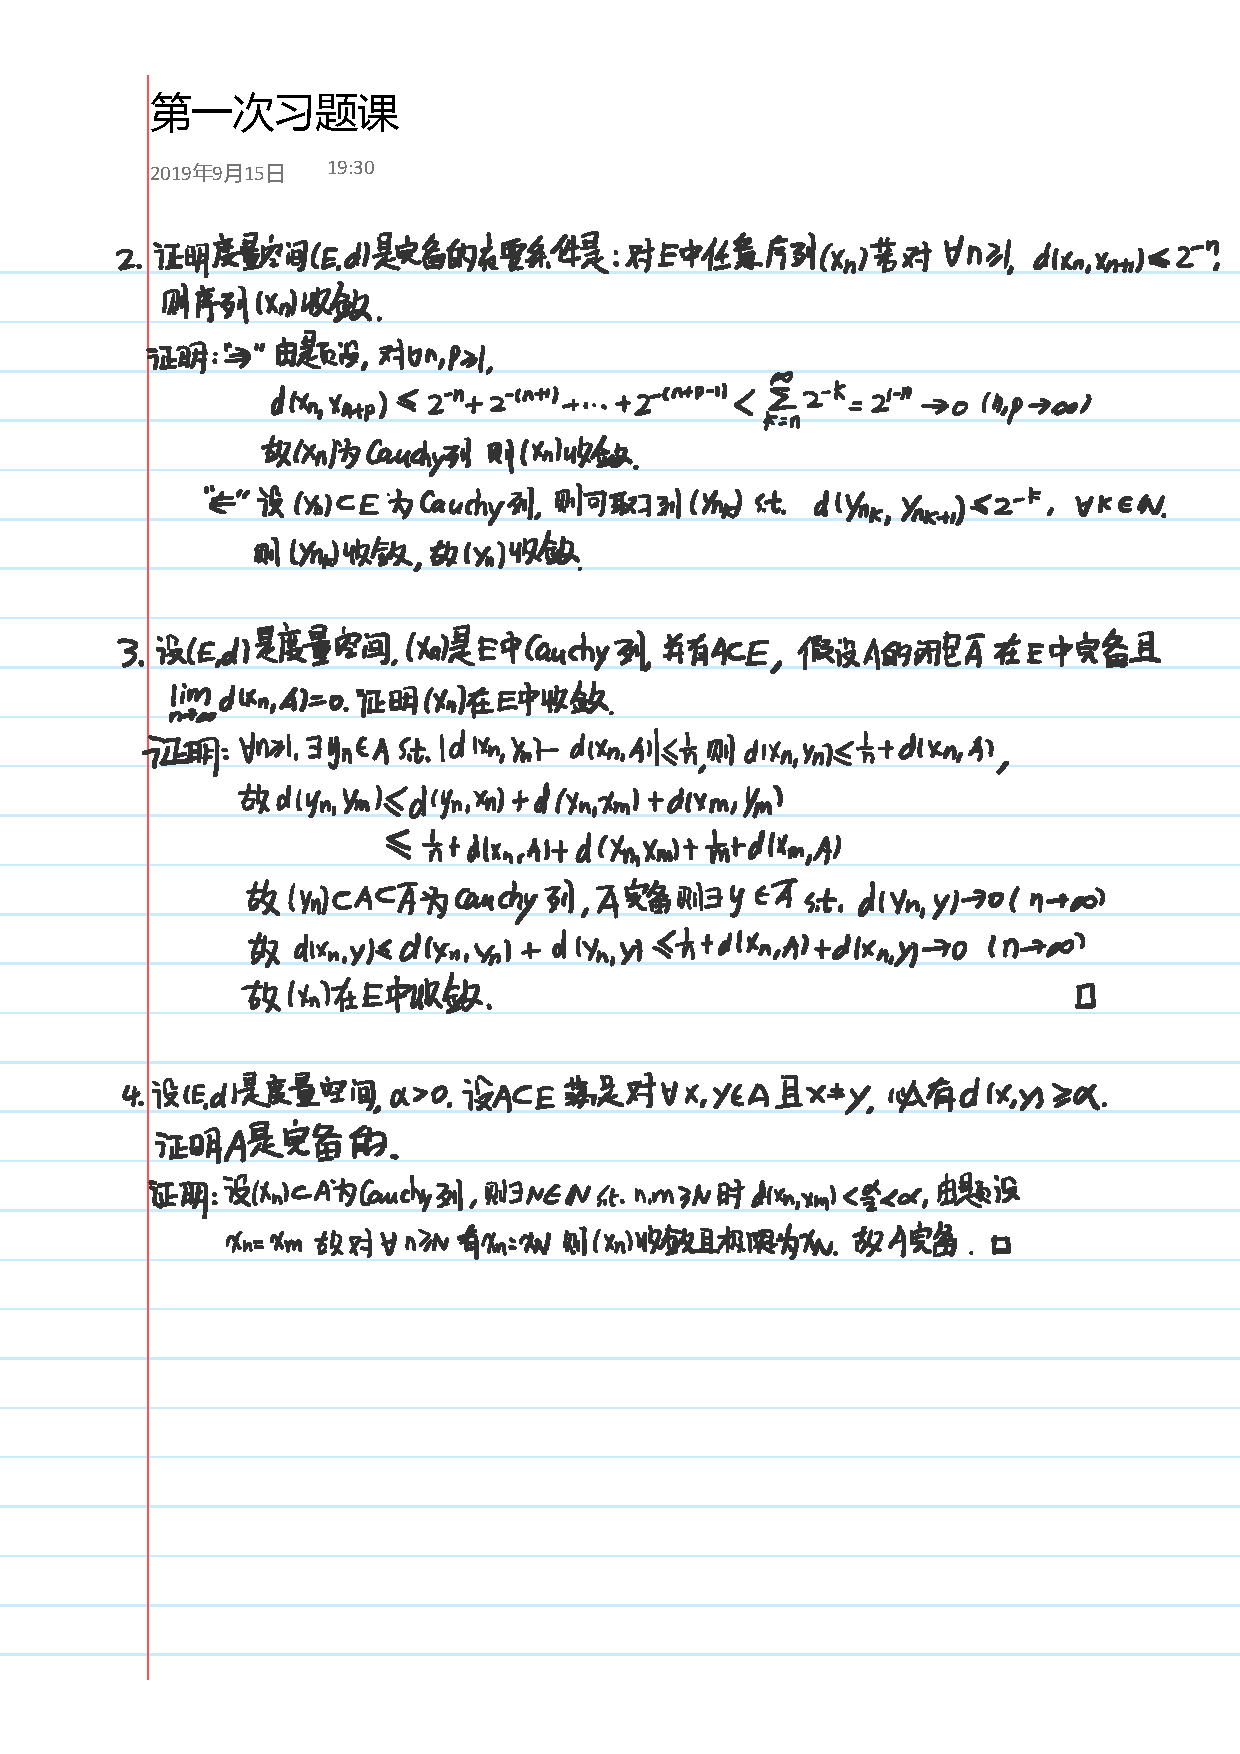
\includepdf[pages={1-1}]{2_1.pdf}

4. 证明紧空间中任一序列有收敛子列。
\begin{proof}
	设$E$是紧空间,序列$(x_n)\subset E$. 若$(x_n)$中只有有限个不同的点,那么一定有收敛子列。
	
	若$(x_n)$中有无限个不同的点。反证,若$(x_n)$无收敛子列,那么,对任意$x\in E$, 存在$U_x\in\mathcal{N}(x)$, s.t. $U_x\backslash\{x\}\cap (x_n)=\varnothing$, $E\subset\cup_{x\in E}U_x$, 由于$E$紧,存在有限个$y_i\in E$, $E\subset \cup_{i=1}^n U_{y_i}$, 则$E$中至多有有限个$(x_n)$的点,这与$(x_n)$有无限多个不同的点相矛盾。
\end{proof}

\section{第二章 习题}
%本章的主要内容:
%\begin{itemize}
%	\item 度量空间,完备性.
%	\item 一致连续映射,不动点定理.
%	\item 完备化.
%	\item 紧性,列紧性,序列紧.
%\end{itemize}
%
%\begin{Def}[度量空间]
%	设$E$是一个非空集合,$d$是定义在$E\times E$上的实值函数,若任意$x,y,z\in E$, 满足
%    \begin{enumerate}
%    	\item[(1)] 非负性:$d(x,y)\geq 0$;
%    	\item[(2)] 正定性:$d(x,y)=0$当且仅当$x=y$;
%    	\item[(3)] 对称性:$d(x,y)=d(y,x)$;
%    	\item[(4)] 三角形不等式:$d(x,y)\leq d(x,z)+d(z,y),$
%    \end{enumerate}
%则称$d$是集合$E$上的一个度量(或称距离),并称$(E,d)$为度量空间。
%\end{Def}
%
%\begin{Def}[一致连续]
%	设$(E,d)$和$(F,\delta)$是两个度量空间,若映射$f:E\to F$满足:对任意$\e>0$, 存在$\eta>0$, 使得当$d(x,y)<\delta$时,必有$\delta(f(x),f(y))<\e$, 则称$f$是一致连续的。
%\end{Def}

6. [作业]设$(E,d)$是度量空间,而$(x_n)$是$E$中发散的Cauchy列。证明
\begin{enumerate}
	\item[(a)] 任取$x\in E$, 序列$(d(x,x_n))$收敛于一个正数,记为$g(x)$.
	\item[(b)] 函数$x\mapsto \frac{1}{g(x)}$是从$E$到$\mathbb{R}$的连续函数。
	\item[(c)] 上面的函数无界。
\end{enumerate}
\begin{proof}
	(a) 由$d$的三角形不等式
	$$|d(x,x_n)-d(x,x_m)|\leq d(x_n,x_m)\to 0(n,m\to\infty),$$
	故$(d(x,x_n))$是$\mathbb{R}$中的Cauchy列,因此存在$\lambda\geq 0$, 使得$d(x,x_n)\to\lambda(n\to\infty)$. 若$\lambda=0$, 则$x_n$在$E$中收敛,与题设矛盾,因此$\lambda>0$, 所以序列$(d(x,x_n))$收敛于一个正数。
	
	(b) 只需证$g(x)$是连续函数。由$d$的三角形不等式,对于任意$x,y\in E$, 任意$n\in \mathbb{N}$, 
	$$|d(x,x_n)-d(y,x_n)|\leq d(x,y),$$
	令$n\to\infty$, 则$|g(x)-g(y)|\leq d(x,y)$, 故$g$为$E$到$\mathbb{R}$的一致连续函数。
	
	(c) 只需证明对任意$\e>0$, 存在$x_{\e}$, 使得$g(x_\e)\leq\e$. 实际上,由于$(x_n)$是Cauchy列, 对任意$\e>0$, 存在$N$, 当$n,m\geq N$时,$d(x_n,x_m)<\e$, 则$\lim_{n\to\infty}d(x_n,x_N)\leq \e$, 即$g(x_N)\leq \e$, 取$x_\e=x_N$即可。
\end{proof}

8. [作业]设$f:\mathbb{R}^n\to\mathbb{R}$是一致连续函数。证明存在两个非负常数$a$和$b$, 使得
$$|f(x)|\leq a\|x\|+b,$$
这里$\|x\|$是$x$的欧氏范数。
\begin{proof}
	由于$f$是一致连续的,取$\e=1$, 存在$\delta>0$, 当$\|x-y\|<\delta$时,$|f(x)-f(y)|<1$. 现在,对于任意$x\in\mathbb{R}^n$, 在连接原点$0$和$x$的直线上等间距地取点$x_i,i=0,1,2,\cdots,n+1$, 使得
	$$x_0=0,x_1=\delta\frac{x}{\|x\|},x_2=2\delta\frac{x}{\|x\|},\cdots,x_n=n\delta\frac{x}{\|x\|},x_{n+1}=x,$$
	且$n$满足$n\delta\leq \|x\|<(n+1)\delta$, 那么利用三角形不等式得
	\[\begin{split}
	|f(x)-f(0)|\leq& |f(x_1)-f(x_0)|+|f(x_2)-f(x_1)|+\cdots+|f(x_n)-f(x_{n-1})|+|f(x_{n+1})-f(x_n)|\\
	< & \frac{1}{\delta}(\delta+\cdots+\delta)+1=\frac{1}{\delta}(n\delta)+1\leq \frac{1}{\delta}\|x\|+1,
	\end{split}\]
	再利用一次三角形不等式得
	$$|f(x)|\leq |f(0)|+|f(x)-f(0)|\leq \frac{1}{\delta}\|x\|+|f(0)|+1.$$
	取$a=1/\delta, b=|f(0)|+1$就证明了结论。
\end{proof}

10. [作业]构造一个反例说明:在不动点定理中,如果我们把映射$f$满足的条件减弱为
$$d(f(x),f(y))<d(x,y),\quad\forall x,y\in E\mbox{ 且 }x\ne y,$$
则结论不成立。\\
提示:考虑函数$f(x)=(x^2+1)^{\frac{1}{2}}$, $x\in[0,+\infty)$.
\begin{proof}
	对于$f(x)=(x^2+1)^{\frac{1}{2}}$, 求导得$f'(x)=\frac{x}{\sqrt{x^2+1}}$,因此
	$$|f'(x)|<1,x\in[0,\infty),$$
	利用Lagrange中值定理,这意味着$d(f(x),f(y))<d(x,y),\forall x,y\in E\mbox{ 且 }x\ne y$. 但是$x=f(x)$不可能成立,否则, $x=(x^2+1)^{\frac{1}{2}}$, 进而$0=1$, 矛盾。 
\end{proof}

10'. [习题课]设$E$为紧的完备度量空间,在不动点定理中,如果我们把映射$f$满足的条件减弱为
$$d(f(x),f(y))<d(x,y),\quad\forall x,y\in E\mbox{ 且 }x\ne y,$$
那么$f$仍然存在唯一不动点。
\begin{proof}
	设$g(x)=d(x,f(x)), x\in E$, 由于$f(\cdot),d(\cdot,\cdot)$都是连续函数,复合函数仍连续,故$g:E\to \mathbb{R}$是连续函数。又由于$E$是紧的,那么$g(E)$是$\mathbb{R}$中的紧集,则$g(E)$是$\mathbb{R}$中的有界闭集,这意味着函数$g$在$E$上存在最小值。设$x_0\in E$是$g$的最小值点,若$x_0\ne f(x_0)$, 则
	$$d(x_0,f(x_0))\leq d(f(x_0),f(f(x_0)))<d(x_0,f(x_0))$$
    矛盾,因此$x_0=f(x_0)$. 
    
    $f$的不动点是唯一的。实际上,若还有一个不动点$y_0$, 则$f(y_0)=y_0$, 那么若$x_0\ne y_0$, 则由题设知$d(x_0,y_0)=d(f(x_0),f(y_0))<d(x_0,y_0)$, 矛盾,所以$x_0=y_0$.
\end{proof}

11. [习题课]设$(E,d)$是一个完备的度量空间,$f$是其上的映射,并满足$f^n=f\circ\cdots\circ f$($n$次幂)是压缩映射。证明$f$有唯一的不动点,并给出例子说明$f$可以不连续。
\begin{proof}
	由于$f^n$是压缩映射,则由不动点定理,$f^n$存在唯一的不动点$x_0$, 即$f^n(x_0)=x_0$, 则
	$$f^n(f(x_0))=f(f^n(x_0))=f(x_0)$$
	所以$f(x_0)$也是$f^n$的不动点,由不动点的唯一性,则$f(x_0)=x_0$, 故$x_0$是$f$的不动点. 
	
	下面再证$x_0$是$f$的唯一不动点,若还有$y_0$使得$f(y_0)=y_0$, 则$f^n(y_0)=y_0$, 即$y_0$是$f^n$的不动点,则$x_0=y_0$.
	
	$f$可以不连续的例子:设$E=[0,1]$, $E$上的函数$f$定义为
	\[f(x)=\begin{cases}
	1, & x\in Q\\
	0, & x\notin Q
	\end{cases}\]
	则$f$不连续,但$f^2$为压缩映射。
\end{proof}

12. [作业]记区间$I=(0,\infty)$上通常的拓扑为$\tau$.
\begin{enumerate}
	\item[(a)] 证明$\tau$可由如下完备的距离$d$诱导:
	$$d(x,y)=|\log x-\log y|.$$
	\item[(b)] 设函数$f:I\to I$且$f\in C^1(I)$, 满足对某个$\lambda<1$,任取$x\in I$, 都有$x|f'(x)|\leq \lambda f(x)$. 证明$f$在$I$上存在唯一的不动点。
\end{enumerate}
\begin{proof}
	(a) 先证明$d$是$I$上的距离,
	\begin{itemize}
		\item $d(x,y)\geq 0$. 显然。
		\item $d(x,y)=0\Leftrightarrow x=y$.  
		$$d(x,y)=0\Leftrightarrow \log x=\log y\Leftrightarrow x=y.$$
		\item $d(x,y)=d(y,x)$, 显然。
		\item $d(x,y)\leq d(x,z)+d(z,y)$. 只需借助$\mathbb{R}$上的三角形不等式,
		$$d(x,y)=|\log x-\log y|\leq |\log x-\log z|+|\log z-\log y|=d(x,z)+d(z,y).$$ 
	\end{itemize}
    因此$d$是$I$上的距离。
    
    再证明$d$是完备的,设$(x_n)$是$(I,d)$中的Cauchy列,即$d(x_n,x_m)\to 0(n,m\to\infty)$, 即$|\log x_n-\log x_m|\to 0(n,m\to \infty)$, 这意味着$(\log x_n)$是$\mathbb{R}$中的Cauchy列。由$\mathbb{R}$完备知,存在$z\in\mathbb{R}$, s.t. $|\log x_n-z|\to 0(n\to \infty)$, 即$|\log x_n-\log e^z|\to 0(n\to \infty)$, 因此$d(x_n,e^z)\to 0(n\to\infty)$, 故$d$是完备的。
    
    最后证明$\tau$可以由$d$诱导,对任意$r>0,x\in I$, 考虑$(I,d)$中的开球$B_d(x,r)$. 由定义$B_d(x,r)=\{y:|\log y-\log x|<r\}$, 由于
    $$|\log y-\log x|<r\Leftrightarrow y\in(xe^{-r},xe^r),$$
    故$B_d(x,r)=(xe^{-r},xe^r)$. 另一方面,对于任意开区间$(a,b)\subset I$, 设$x=\sqrt{ab}, y=\frac{1}{2}\log \frac{b}{a}$, 则$(a,b)=(xe^{-r},xe^r)$. 因此$\tau$可以由$d$诱导。
    
    (b) 可以证明$f$是$(I,d)$上的压缩映射,即存在$0\leq \lambda<1$, 使得
    $$|\log f(x)-\log f(y)|<\lambda|\log x-\log y|.$$
    这可以用两种方法证明。
    
    \textbf{法I}: 由Cauchy中值定理,对任意$x,y\in I$, 存在$\xi\in(x,y)$, s.t.
    $$\frac{\log f(x)-\log f(y)}{\log x-\log y}=\left.\frac{(\log[f(x)])'}{(\log x)'}\right|_{x=\xi}=\frac{\frac{f'(\xi)}{f(\xi)}}{\frac{1}{\xi}},$$
    再结合已知条件知
    $$\left|\frac{\log f(x)-\log f(y)}{\log x-\log y}\right|\leq \lambda.$$
    
    \textbf{法II}: 由题设知
    $$\pm \frac{f'(t)}{f(t)}\leq \lambda \frac{1}{t}, t\in I$$
    两边同时在$[x,y]$上积分,则
    $$\pm (\log f(y)-\log f(x))\leq \lambda(\log y-\log x),$$
    这意味着$|\log f(y)-\log f(x)|\leq \lambda|\log y-\log x|$.
    
    因此$f:I\to I$是完备度量空间$(I,d)$上的压缩映射,所以$f$在$I$上存在唯一的不动点。
\end{proof}
\begin{Remark}
	12题中,$I$上原来的度量与新定义的度量$d$诱导的拓扑相同。$I$上原来的度量是不完备的,但新定义的度量$d$是完备的,这表明完备性不是一个拓扑概念。
\end{Remark}

13. [习题课]设$E$为可数集,其元素记为$a_1,a_2,\cdots$(两两不同). 定义
\[d(a_p,a_q)=\begin{cases}
0, & p=q\\
10+\frac{1}{p}+\frac{1}{q}, & p\ne q
\end{cases}\]
\begin{enumerate}
	\item[(a)] 证明$d$是$E$上的距离并且$E$成为一个完备的度量空间。
	\item[(b)] 设$f:E\to E$定义为$f(a_p)=a_{p+1}$. 证明当$p\ne q$时,有
	$$d(f(a_p),f(a_q))<d(a_p,a_q),$$
	但是$f$没有不动点。
\end{enumerate}
\begin{proof}
	(a) 易证$d$是$E$上的距离,下证$(E,d)$是完备的。设有$E$中的Caushy列$(a_{p(n)})$, 则$\forall\e>0$, 存在$N$, 当$m,n\geq N$时,$d(a_{p(m)},a_{p(n)})<\e$. 取$\e<10$, 则由于
	\[d(a_{p(m)},a_{p(n)})=\begin{cases}
	0, & p(m)=p(n)\\
	10+\frac{1}{p(m)}+\frac{1}{p(n)}, & p(m)\ne p(n)
	\end{cases}\]
	那么$p(m)=p(n),n,m\geq N$, 这意味着对任意$n\geq N$, $p(n)=p(N)$, 故
	$$a_{p(n)}\to a_{p(N)}(n\to\infty),$$
	所以$(E,d)$完备。
	
	(b) 当$p\ne q$时,
	$$d(f(a_p),f(a_q))=d(a_{p+1},a_{q+1})=10+\frac{1}{p+1}+\frac{1}{q+1}<10+\frac{1}{p}+\frac{1}{q}=d(a_p,a_q).$$
	
	若$f$有不动点$a_p$, 即$f(a_p)=a_p$, 即$a_{p+1}=a_{p}$, 矛盾。
\end{proof}

14. 本习题的目的是给出不动点定理的一个新的证明方法. 设$(E,d)$是非空的完备度量空间,$f:E\to E$是压缩映射. 任取$R\geq 0$, 设
$$A_R=\{x\in E:d(x,f(x))\leq R\}.$$
\begin{enumerate}
	\item[(a)] 证明$f(A_R)\subset A_{\lambda R}$.
	\item[(b)] 证明当$R>0$时,$A_R$是$E$中的非空闭子集.
	\item[(c)] 证明任取$x,y\in A_R$, 有$d(x,y)\leq 2R+d(f(x),f(y))$. 并由此导出
	$$\mathrm{diam}(A_R)\leq \frac{2R}{1-\lambda}.$$
	\item[(d)] 证明$A_0$非空.
\end{enumerate}
\begin{proof}
	(a) 设$x\in A_R$, 即$d(x,f(x))\leq R$, 则
	$$d(f(x),f(f(x)))\leq \lambda d(x,f(x))\leq \lambda R,$$
	故$f(x)\in A_{\lambda R}$, 所以$f(A_R)\subset A_{\lambda R}$.
	
	(b) 由$f,d$的连续性知$A_R$是闭的。
	
	设$R>0$, 下证$A_R$非空。 对任意$x\in E$, $d(f(x),f(f(x)))\leq \lambda d(x,f(x))$, $d(f^2(x),f^2(f(x)))\leq \lambda^2d(x,f(x))$, $\cdots$, 依此类推,对任意$n\in\mathbb{N}$, 有
	$$d(f^n(x),f^n(f(x)))\leq \lambda^n d(x,f(x)),$$
	由于$\lambda\in[0,1)$, 存在$N$, 当$n\geq N$时,$\lambda^n d(x,f(x))<R$, 取$z=f^N(x)$, 则有$d(z,f(z))<R$, 因此$A_R$非空。
	
	(c) 任取$x,y\in A_R$, 则$d(x,f(x))\leq R$, $d(y,f(y))\leq R$, 则
	$$d(x,y)\leq d(x,f(x))+d(f(x),f(y))+d(f(y),y)\leq 2R+d(f(x),f(y)).$$
	进一步
	$$d(x,y)\leq 2R+d(f(x),f(y))\leq 2R+\lambda d(x,y),$$
	因此$d(x,y)\leq \frac{2R}{1-\lambda}$, 那么由定义知$\mathrm{diam}(A_R)\leq \frac{2R}{1-\lambda}$.
	
	(d) 注意到$A_0=\{x\in E:d(x,f(x))=0\}$可以写成
	$$A_0=\{x\in E:d(x,f(x))\leq \frac{1}{n},\forall n\in \mathbb{N}\}=\cap_{n\geq 1}A_{\frac{1}{n}}.$$
	由(b)知对于每个$n$, $A_{\frac{1}{n}}$是非空闭集,故$(A_{\frac{1}{n}})$是$E$中单调下降的非空闭子集列,且由(c)知$\lim_{n\to\infty}\mathrm{diam}(A_{\frac{1}{n}})=0$, 由定理2.2.6知$\cap_{n\geq 1}A_{\frac{1}{n}}$是单点集,所以$A_0$非空。
\end{proof}

15. [作业]设$(E,d)$是完备度量空间,$f$和$g$是$E$上两个可交换的压缩映射(即$f\circ g=g\circ f$). 证明$f$和$g$有唯一的、共同的不动点。\\
通过反例说明如果去掉可交换的条件,则结论不成立。
\begin{proof}
	设$f$的不动点为$x_0$, 即$x_0=f(x_0)$, 则
	$$g(x_0)=g(f(x_0))=f(g(x_0)),$$
	这意味着$g(x_0)$也是$f$的不动点,因此$g(x_0)=x_0$. 
	
	反例:$E=[0,1]$, $f(x)\equiv\frac{1}{4}$, $g(x)\equiv\frac{3}{4}$, 则$f[g(x)]\equiv \frac{1}{4},g[f(x)]\equiv\frac{3}{4}$, 所以$f$与$g$不交换,$f,g$的不动点分别为$\frac{1}{4},\frac{3}{4}$.
\end{proof}
\clearpage
\section{第三章 习题}
1. [作业]设$C([0,1],\mathbb{R})$表示$[0,1]$上所有的连续实函数构成的空间。定义
$$\|f\|_\infty=\sup_{0\leq t\leq 1}|f(t)|\mbox{ 且 }\|f\|_1=\int_0^1|f(t)|dt.$$
\begin{enumerate}
	\item[(a)] 证明$\|\cdot\|_\infty$和$\|\cdot\|_1$都是$C([0,1],\mathbb{R})$上的范数。
	\item[(b)] 证明$C([0,1],\mathbb{R})$关于范数$\|\cdot\|_\infty$是完备的。
	\item[(c)] 证明$C([0,1],\mathbb{R})$关于范数$\|\cdot\|_1$不完备。
\end{enumerate}
\begin{proof}
	(a) $\|\cdot\|_\infty$是$C([0,1],\mathbb{R})$上的范数:
	\begin{itemize}
		\item $\|f\|_\infty=0\Leftrightarrow f(t)\equiv 0,\forall t\in[0,1]$,
		\item $\|\lambda f\|_\infty=|\lambda|\|f\|_\infty$, 显然,
		\item $\|f+g\|_\infty=\sup_{0\leq t\leq 1}|f(t)+g(t)|\leq \sup_{0\leq t\leq 1}|f(t)|+\sup_{0\leq t\leq 1}|g(t)|=\|f\|_\infty+\|g\|_\infty$.
	\end{itemize}
    所以$\|\cdot\|_\infty$是$C([0,1],\mathbb{R})$上的范数。
    
    $\|\cdot\|_1$是$C([0,1],\mathbb{R})$上的范数:
    \begin{itemize}
    	\item $\|f\|_1=0\Leftrightarrow f(t)\equiv 0,\forall t\in[0,1]$,
    	\item $\|\lambda f\|_1=|\lambda|\|f\|_1$, 显然,
    	\item $\|f+g\|_1=\int_0^1 |f(t)+g(t)|dt\leq\int_0^1|f(t)|dt+\int_0^1|g(t)|dt =\|f\|_1+\|g\|_1$.
    \end{itemize}
    所以$\|\cdot\|_1$是$C([0,1],\mathbb{R})$上的范数。
    
    (b) 设$(f_n)$是$C([0,1],\mathbb{R})$中的Cauchy列,则对任意$\e>0$, 存在$N$, 当$n,m\geq N$时,
    \begin{equation}\label{3.1}
    	\|f_n-f_m\|_\infty=\sup_{t\in[0,1]}|f_n(t)-f_m(t)|<\e,\tag{*}
    \end{equation}
    则对于任意$t\in[0,1]$, $(f_n(t))$是$\mathbb{R}$中的Cauchy列,则$(f_n(t))$收敛,设$f(t)=\lim_{n\to\infty}f_n(t)$, 下证$f$是连续的。在\eqref{3.1}中令$m\to\infty$, 则$\|f_n-f\|_\infty\leq \e$. 利用$f_N$的连续性,存在$\delta$, 当$|x-y|<\delta$时,$|f_N(x)-f_N(y)|<\e$, 因此,联合\eqref{3.1}知$|x-y|<\delta$时,
    $$|f(x)-f(y)|\leq |f(x)-f_N(x)|+|f_N(x)-f_N(y)|+|f_N(y)-f(y)|<3\e,$$
    所以$f$连续,故$f\in C([0,1],\mathbb{R})$, 所以范数$\|\cdot\|_\infty$完备。
    
    (c) 设$f_n(t)$为如下分段函数:
    \[f_n(t)=\begin{cases}
    -1, & 0\leq t<\frac{1}{2}-\frac{1}{n}\\
    n(t-\frac{1}{2}), & \frac{1}{2}-\frac{1}{n}\leq t\leq \frac{1}{2}+\frac{1}{n}\\
    1, & \frac{1}{2}+\frac{1}{n}<t\leq 1
    \end{cases}\]
    则$\|f_n-f_m\|_1=|\frac{1}{n}-\frac{1}{m}|\to0$, 故$(f_n)$为$(C([0,1],\mathbb{R}),\|\cdot\|_1)$上的Cauchy列。下面证明这个Cauchy列不收敛。
    
    反证法,若存在$f\in C([0,1],\mathbb{R})$使得$\|f_n-f\|_1\to0$, 则
    \[\|f_n-f\|_1=\int_0^{1/2-1/n}|f(t)+1|dt+\int_{1/2-1/n}^{1/2+1/n}|f(t)-n(t-\frac{1}{2})|dt+\int_{\frac{1}{2}+\frac{1}{n}}^1|f(t)-1|dt\to 0\]
    则$\int_0^{1/2}|f(t)+1|dt+\int_{1/2}^1 |f(t)-1|dt=0$, 这意味着对任意$t\in[0,1/2], $$f(t)=-1$; 对任意$t\in[1/2,1]$, $f(t)=1$, 则$f(1/2)=-1=1$, 矛盾,所以$(f_n)$在范数$\|\cdot\|_1$下不收敛,所以$C([0,1],\mathbb{R})$关于范数$\|\cdot\|_1$不完备。
\end{proof}

2. [习题课]设$E$是$\mathbb{R}$上所有的实系数多项式构成的向量空间。对任一$p\in E$, 定义
$$\|P\|_\infty=\max_{x\in[0,1]}|P(x)|$$
\begin{enumerate}
	\item[(a)] 证明$\|\cdot\|_\infty$是$E$上的范数。
	\item[(b)] 任取一个$a\in\mathbb{R}$, 定义线性映射$L_a:E\to\mathbb{R}$满足$L_a(P)=P(a)$. 证明$L_a$连续当且仅当$a\in[0,1]$, 并且给出该连续线性映射的范数。
	\item[(c)] 设$a<b$并定义$L_{a,b}:E\to\mathbb{R}$满足
	$$L_{a,b}(P)=\int_a^b P(x)dx$$
	给出$a,b$的取值范围,使其成为$L_{a,b}$连续的充分必要条件,然后确定$L_{a,b}$的范数。
\end{enumerate}

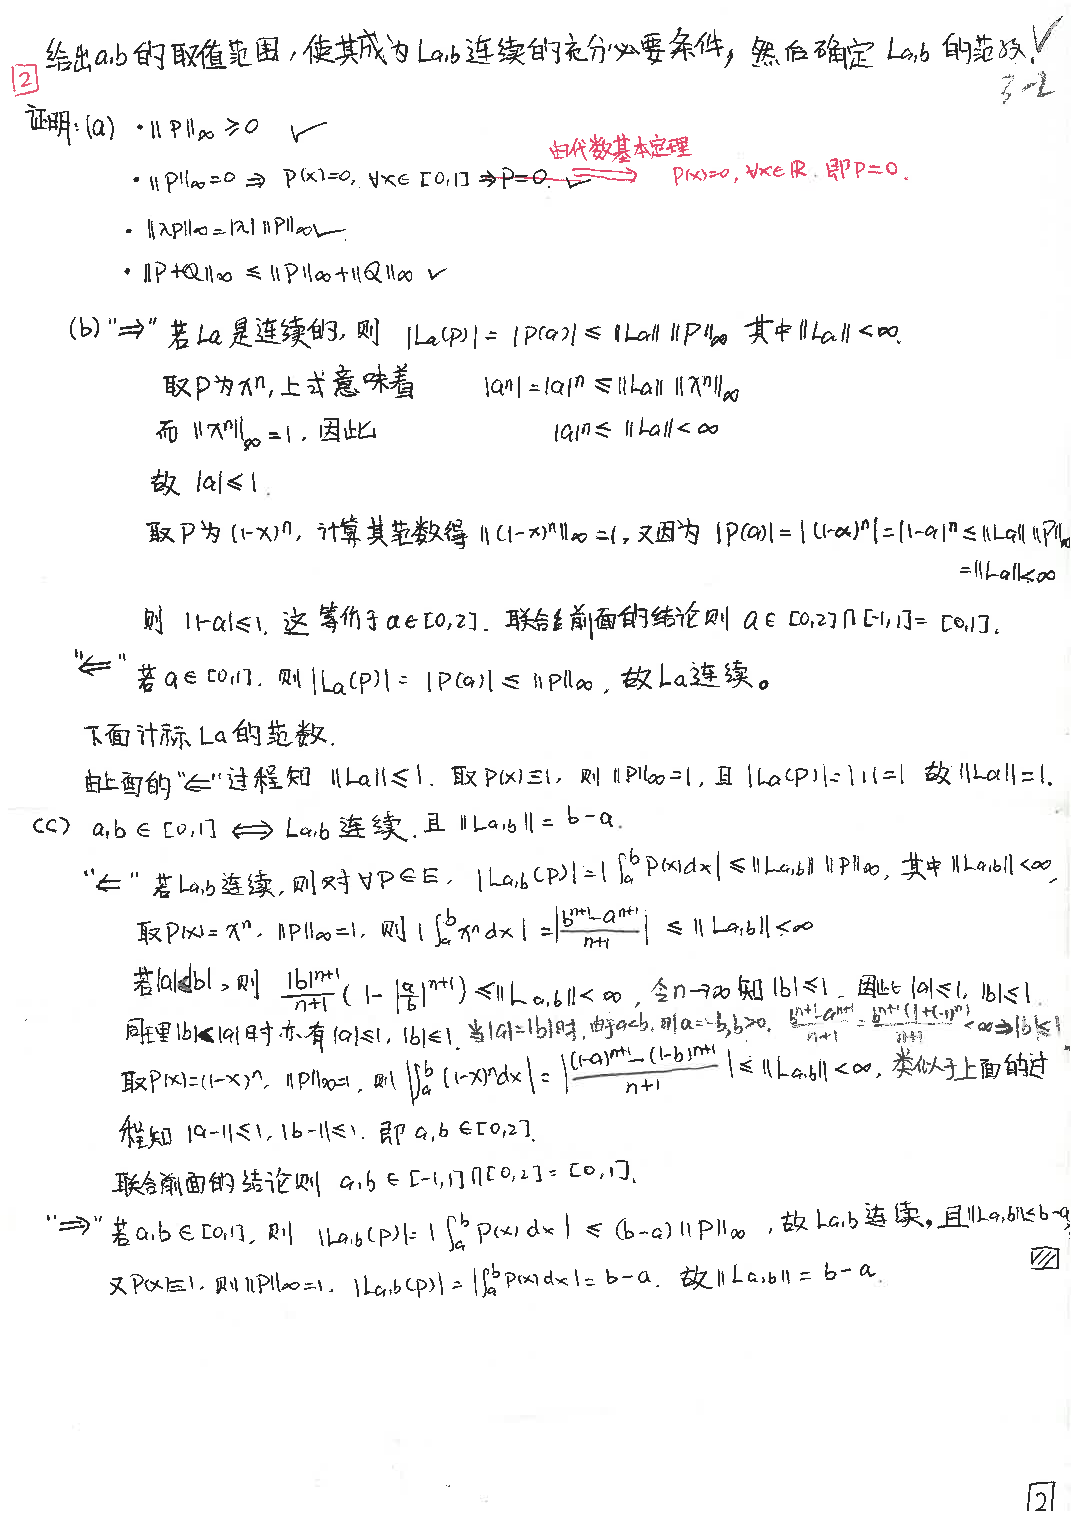
\includepdf[pages={1-1}]{3_2.pdf}
\clearpage
3. [作业题]设$(E,\|\cdot\|_\infty)$是习题2中定义的赋范空间。设$E_0$是$E$中没有常数项的多项式构成的向量子空间(即多项式$P\in E_0$等价于$P(0)=0$).
\begin{enumerate}
	\item[(a)] 证明$N(P)=\|P'\|_\infty$定义了$E_0$上的一个范数,并且对任意$P\in E_0$, 有$\|P\|_\infty\leq N(P)$.
	\item[(b)] 证明$L(P)=\int_0^1 \frac{P(x)}{x}dx$定义了$E_0$上关于$N$的连续线性泛函,并求它的范数。
	\item[(c)] 上面定义的$L$是否关于范数$\|\cdot\|_\infty$连续?
	\item[(d)] 范数$\|\cdot\|_\infty$和$N$在$E_0$上是否等价?
\end{enumerate}
\begin{proof}
	(a) 先证明$N(P)$是$E_0$上的一个范数。
	\begin{itemize}
		\item $N(P)=0\Leftrightarrow P'=0\Leftrightarrow P\equiv C(\mbox{常数})$, 又$P(0)=0$知$C=0$, 故$P\equiv 0$.
		\item $N(\lambda P)=\|(\lambda P)'\|_\infty=|\lambda|\|P'\|_\infty=|\lambda|N(P)$.
		\item $N(P+Q)=\|P'+Q'\|_\infty\leq \|P'\|_\infty+\|Q'\|_\infty=N(P)+N(Q)$.
	\end{itemize}
	故$N(P)$是$E_0$上的一个范数。
	
	设$P\in E_0$, 对任意$x\in[0,1]$, 由Lagrange中值定理,$|\frac{P(x)-P(0)}{x}|=|P'(\xi)|\leq\|P'\|_\infty$, 这里$\xi\in(0,x)$, 则$|P(x)|\leq |x|\|P'\|_\infty\leq \|P'\|_\infty$, 所以$\|P\|_\infty\leq \|P'\|_\infty=N(P)$. 
	
	(b) 显然$L(P)$是线性泛函。任意$x\in[0,1]$, 存在$\xi\in(0,x)$, 使得$\frac{P(x)}{x}=P'(\xi)$, 因此$\sup_{x\in[0,1]}|\frac{P(x)}{x}|\leq \sup_{x\in[0,1]}|P'(x)|$, 则
	$$\left|\int_0^1 \frac{P(x)}{x}dx\right|\leq \sup_{x\in[0,1]}\left|\frac{P(x)}{x}\right|\leq\sup_{x\in[0,1]}|P'(x)|=N(P),$$
	即$L(P)\leq N(P)$, 所以$L$关于范数$N$连续,且$\|L\|\leq 1$, 取$P(x)=x\in E_0$, 则$N(P)=1$, $L(P)=\int_0^1 dx=1$, 则$\|L\|=1$.
	
	(c) $L$关于$\|\cdot\|_\infty$不连续。反证法,假设$L$关于$\|\cdot\|_\infty$连续。设$A=\{f:\in C[0,1]\mbox{ 且 }f(0)=0\}$, 则易验证$A$是一个Banach空间。
	
	下证$E_0$在$A$中稠密,\textbf{法I:} 由Weierstrass逼近定理,对于任意$f\in A\subset C[0,1]$, 可取多项式$P_n$一致逼近$f$, 则$P_n(0)\to 0(n\to\infty)$, 那么$\|P_n-P_n(0)-f\|_{\infty}\to 0(n\to\infty)$, 令$Q_n=P_n-P_n(0)$, 则$Q_n\in E_0$且一致逼近于$f$。
	
	\textbf{法II:} 取Berstein多项式基
	\[b_{v,n}(x)=\begin{pmatrix}
	n\\v
	\end{pmatrix}x^v(1-x)^{n-v}, v=0,1,\cdots,n\]
	构造Berstein多项式
	$$B_n(f)(x)=\sum_{v=0}^n f(\frac{v}{n})b_{v,n}(x),$$
	则由Bernstein定理知
	$$\lim_{n\to\infty}\|B_n(f)-f\|_\infty=0,$$
	而且从上述构造知,若$f(0)=0$, 则相应的多项式$B_n(f)$常数项为0, 所以$A$中的元素可以由$E_0$中的元素一致逼近,这意味着$E_0$在$A$中稠密,因此,利用定理3.2.13, $E_0$上的连续线性泛函$L$可以唯一地拓展为$A$上的连续线性泛函,记为$\tilde{L}$. 取$A$中的元素$f(x)=x^{1/n}$, $\|f\|=1$, 且$\tilde{L}(f)=\int_0^1\frac{x^{1/n}}{x}dx=n$, 则$\tilde{L}$关于$\|\cdot\|_\infty$不连续,矛盾。
	
	(d) 若范数$\|\cdot\|_\infty$和$N$在$E_0$上等价,则恒等映射$I_{E_0}:(E_0,\|\cdot\|_\infty)\to(E_0,N)$是连续的。设$P(x)=x^n, n\in\mathbb{N}$, 则$\|P\|_\infty=1$, 但是$N(P)=\|P'\|_\infty=\|nx^{n-1}\|_\infty=n$, 因此对任意$n\in\mathbb{N}$有$\|I_{E_0}\|\geq n$,这与$I_E$的连续性矛盾,所以范数$\|\cdot\|_\infty$和$N$在$E_0$上不等价。
\end{proof}
4. 设$E$是由$[0,1]$上所有连续函数构成的向量空间。定义$E$上的两个范数分别为$\|f\|_1=\int_0^1 |f(x)|dx$和$N(f)=\int_0^1 x|f(x)|dx$.
\begin{enumerate}
	\item[(a)] 验证$N$的确是$E$上的范数且$N\leq \|\cdot\|_1$.
	\item[(b)] 设函数$f(x)=n-n^2x$, 若$x\leq\frac{1}{n}$; $f_n(x)=0$, 其他。证明函数列$(f_n)_{n\geq 1}$在$(E,N)$中收敛到$0$. 它在$(E,\|\cdot\|_1)$中是否收敛?由这两个范数在$E$上诱导的拓扑是否相同?
	\item[(c)] 设$a\in(0,1]$, 并令$B=\{f\in E:f(x)=0,\forall x\in[0,a]\}$. 证明这两个范数在$B$上诱导相同的拓扑。
\end{enumerate}
\begin{proof}
	(a) 先证明$N$是$E$上的一个范数。
	\begin{itemize}
		\item $N(f)=0\Leftrightarrow xf(x)\equiv0\Leftrightarrow f\equiv 0$.
		\item $N(\lambda f)=|\lambda|N(f)$, 显然。
		\item $N(f+g)=\leq N(f)+N(g)$, 显然。
	\end{itemize}
	故$N$是$E$上的一个范数。
	
	$N(f)=\int_0^1 x|f(x)|dx\leq \int_0^1 |f(x)|dx=\|f\|_1\Rightarrow N\leq \|\cdot\|_1$.
	
	(b) 由于
	$$N(f_n-0)=\int_0^{1/n} nx(1-nx)dx=\int_0^1 t(1-t)\frac{dt}{n}=\frac{1}{6n}\to 0,$$
	故$(f_n)$在$(E,N)$中收敛到0. 然而,若$(f_n)$在$(E,\|\cdot\|_1)$中收敛,设收敛于$f\in E$, 则
	$$\int_{1/n}^1|f|dx\leq \int_0^{1/n}|n(1-nx)-f(x)|dx+\int_{1/n}^1|f|dx=\|f_n-f\|_1\to 0(n\to\infty),$$
	则$\int_0^1 |f(x)|dx=0$, 这意味着$f\equiv0$. 然而$\|f_n-f\|_1=\|f_n\|=\int_0^{1/n}n(1-nx)dx=\frac{1}{2}\nrightarrow 0$, 矛盾,故$(f_n)$在$(E,\|\cdot\|_1)$中不收敛。这意味着这两个范数在$E$上诱导的拓扑不同。
	
	(c) 只需证明范数$\|\cdot\|_1$与$N$在$B$上等价。
	$$N(f)=\int_0^1 x|f(x)|dx\leq \int_0^1 |f(x)|dx=\|f\|_1\Rightarrow N\leq \|\cdot\|_1,$$
	另一方面,
	$$N(f)=\int_0^1 x|f(x)|dx=\int_a^1 x|f(x)|dx\geq a\int_a^1 |f(x)|dx=a\int_0^1 |f(x)|dx=a\|f\|_1\Rightarrow \|\cdot\|_1\leq \frac{1}{a}N,$$
	故
	$$N\leq \|\cdot\|_1\leq \frac{1}{a}N$$
	所以$\|\cdot\|_1$与$N$在$B$上等价。
\end{proof}

\includepdf[pages={1-2}]{3_1.pdf}

7. 设$E$是数域$\mathbb{K}$上的无限维向量空间。设$(e_i)_{i\in I}$是$E$中的一组向量。若$E$中任意向量可用设$(e_i)_{i\in I}$中有限个向量唯一线性表示,则称$(e_i)_{i\in I}$是$E$中一个Hamel基。

\noindent (a) 由Zorn引理证明$E$有一组Hamel基。\\
\noindent (b) 假设$E$还是一个赋范空间,证明$E$上必存在不连续的线性泛函。\\
\noindent (c) 证明在任一无限维赋范空间上,一定存在一个比原范数严格强的范数(即新范数诱导的拓扑比原来的范数诱导的拓扑强且不同). 由此说明,若向量空间$E$上任意两个范数诱导同一个拓扑,$E$必为有限维空间。
\begin{Lemma}[Zorn]
	在任何一个非空的偏序集中,如果任何全序子集都有上界,那么这个偏序集存在一个极大元。
\end{Lemma}
\begin{proof}
	(a) 记$\mathcal{F}=\{F\subset E\text{ 为线性子空间}:F\text{ 含有Hamel基}\}$. 由于任意有限维子空间必含有Hamel基故$\mathcal{F}$非空。设$F\in\mathcal{F}$的一个Hamel基为$(f_i)_{i\in I}$, 令$\mathcal{G}=\{(F,(f_i)_{i\in I}),F\in \mathcal{F}\}$. 定义$\mathcal{G}$上的序"$\leq$"为
	\begin{equation*}
	(F,(f_i)_{i\in I})\leq (G,(g_j)_{j\in J})\Leftrightarrow F\subset G\text{ 且}(f_i)_{i\in I}\subset (g_j)_{j\in J}
	\end{equation*}
	设$\{(F_k, (a_{kj}))\}\subset \F$为全序子集,令$F=\cup_{k}F_k$, $(a_i)=\cup_{k}(a_{kj})$, 显然$F$为线性空间且$(a_i)$为$F$的Hamel基,故$(F,(a_i))$是$\{(F_k, (a_{kj}))\}$的上界,由Zorn引理,$\mathcal{G}$有极大元$(G,(g_j))$. 下证$G=E$, 否则若$G\neq E$, 则存在$x\in E, x\notin G$, 则$x$不能由$(g_j)$中的元素线性表出,故$G\subsetneqq G+\mathbb{K}x$且$(g_j)\cup\{x\}$是$G+\mathbb{K}x$的Hamel基,这与$(G,(g_j))$的极大性矛盾, 故$E$有Hamel基$(g_j)$.
	
	(b) 设$(e_i)_{i\in I}$是$E$的Hamel基,任取$e_1\in(e_i)_{i\in I}$, $E$为无限维则存在$e_2\in(e_i)_{i\in I}$使得$\{e_1,e_2\}$线性无关,同理存在$e_3\in(e_i)_{i\in I}$使得$\{e_1,e_2, e_3\}$线性无关, 依此类推得到一个线性无关序列$(e_n)\subset (e_i)_{i\in I}$, 除上述取得的$e_n$外$(e_i)_{i\in I}$中其他元素记为$(e_j)_{j\in J}$, 用$\frac{e_n}{n\|e_n\|}$代替$e_n$, 仍然记为$e_n$, 则$(e_i)_{i\in I}=(e_n)_{n\geq 1}\cup (e_j)_{j\in J}$仍为Hamel基。对任意$x\in E$, $x=\sum_ix_ie_i$ (除有限项之外均为0), 令映射
	\begin{equation*}
	f:E\to \mathbb{K}, f(x)=\sum_i x_i.
	\end{equation*}
	显然$f$为$E$上的线性泛函, 注意到$f(e_n)=1, \forall n\geq 1$但$e_n\to 0(n\to\infty)$, 故$f$不连续。
	
	(c) 设$E$上的原范数为$\|\cdot\|$, 将(b)中找到的不连续泛函记为$f$. 令
	$$\|x\|_1=\|x\|+|f(x)|,\forall x\in E$$ 易看出$\|\cdot\|_1$为$E$上的范数且$\|x\|\leq \|x\|_1$, 故$\|\cdot\|_1$诱导的拓扑更强,又由于存在$(e_n)_{n\geq 1}$使得$\|e_n\|\to 0$且$|f(e_n)|=1$, 则$\|e_n\|_1=\|e_n\|+|f(e_n)|\nrightarrow 0$, 故$\|\cdot\|_1$与$\|\cdot\|$诱导不同的拓扑。
\end{proof}

8. [习题]设$E$为数域$\mathbb{K}$上的有限维向量空间,其维数$\dim E=n$. $\{e_1,\cdots,e_n\}$表示$E$的一组基。任取$u\in\mathcal{L}(E)$, 令$[u]$表示$u$在这组基下对应的矩阵。
\begin{itemize}
	\item[(a)] 证明映射$u\mapsto[u]$建立了从$\mathcal{L}(E)$到所有$n\times n$矩阵构成的向量空间$\mathbb{M}_n(\mathbb{K})$之间的同构映射。
	\item[(b)] 假设$E=\mathbb{K}^n$且$\{e_1,\cdots,e_n\}$是经典基。并约定$E=\mathbb{K}^n$赋予欧氏范数。证明若$u$(或等价的$[u]$)可对角化,则$\|u\|=\max\{|\lambda_1|,\cdots,|\lambda_n|\}$, 这里$\lambda_1,\cdots,\lambda_n$是$u$的特征值。
	\item[(c)] $\{e_1,\cdots,e_n\}$如上,试由$[u]$中的元素分别确定在$p=1$和$p=\infty$时$u:(\mathbb{K}^n,\|\cdot\|_p)\to(\mathbb{K}^n,\|\cdot\|_p)$的范数.
\end{itemize}
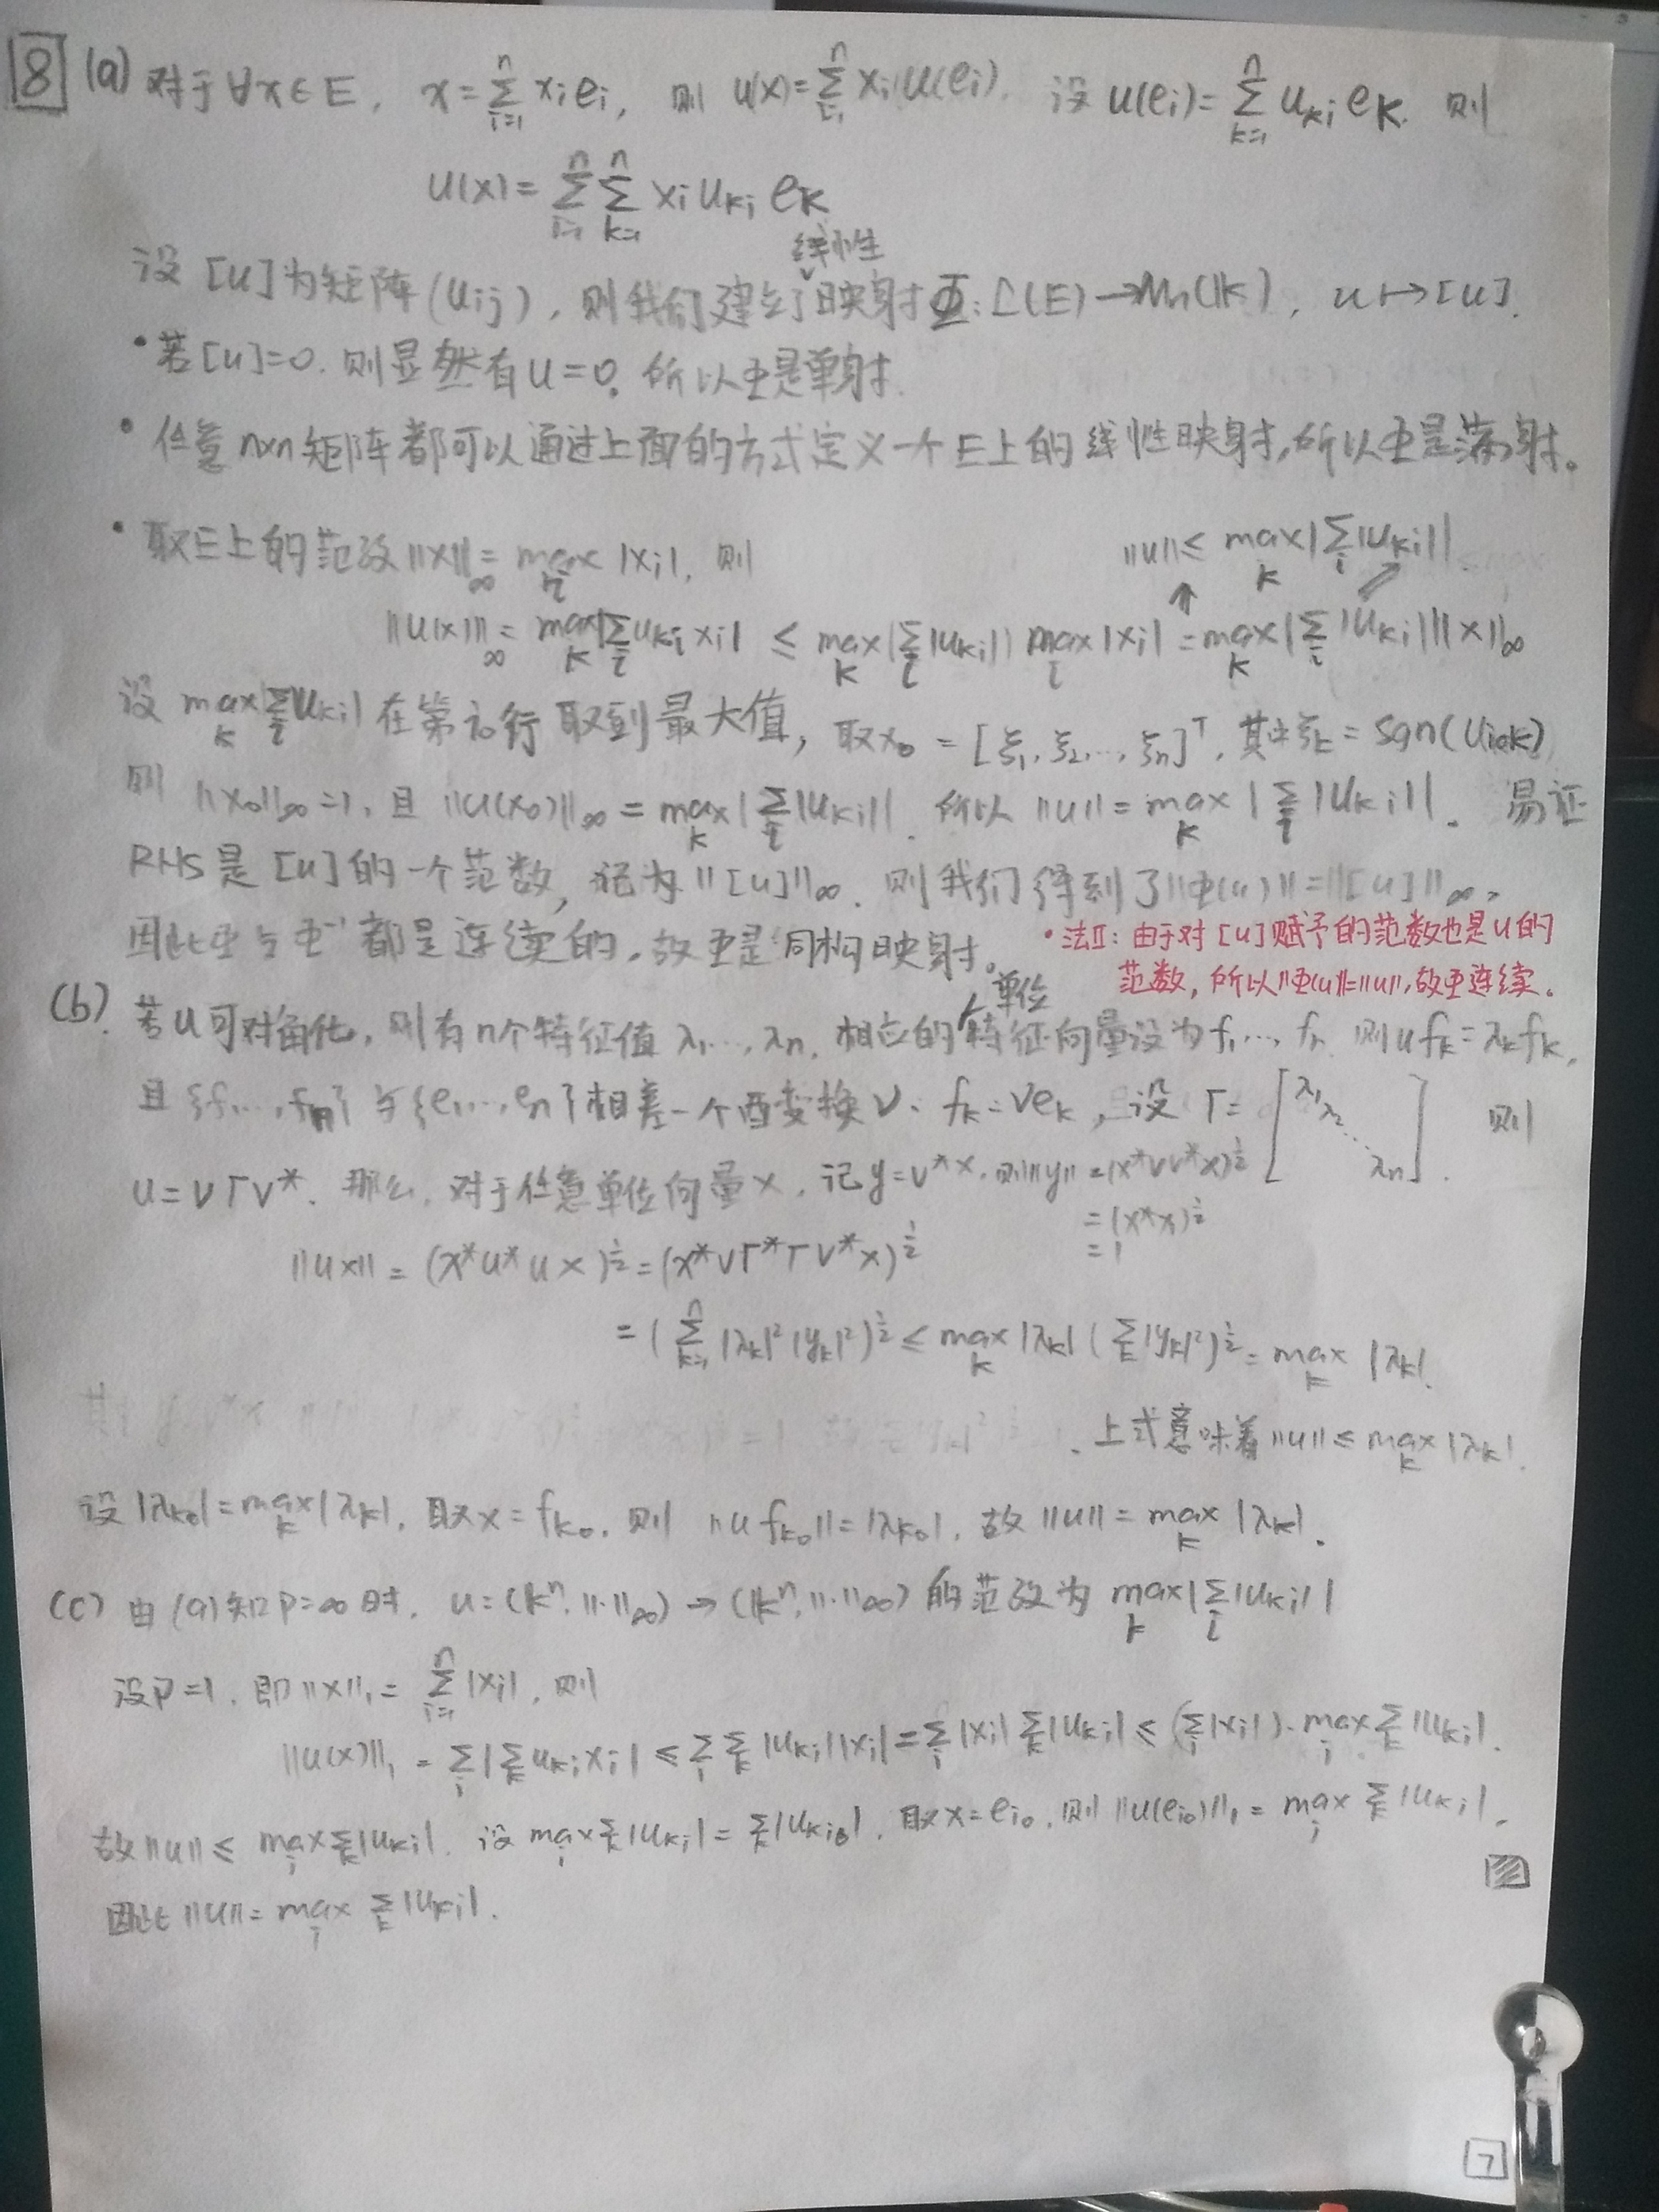
\includegraphics[scale=0.18]{3_8.jpg}
\clearpage
9. [作业]设$E$是Banach空间。
\begin{enumerate}
	\item[(a)] 设$u\in \mathcal{B}(E)$且$\|u\|< 1$. 证明$I_E-u$在$\mathcal{B}(E)$中可逆。
	提示:考虑$\mathcal{B}(E)$中的级数$\sum_{n}u^n$.
	\item[(b)] 设$GL(E)$表示$\mathcal{B}(E)$中可逆元构成的集合。证明$GL(E)$关于复合运算构成一个群且是$\mathcal{B}(E)$中的开集。
	\item[(c)] 证明$u\mapsto u^{-1}$是$GL(E)$上的同胚映射。
\end{enumerate}
\begin{proof}
	(a) 注意到$\|u^n\|\leq \|u\|^n$, 又由于$\|u\|<1$, 那么级数$\sum_{n\geq 0}u^n$绝对收敛,又因为$\mathcal{B}(E)$完备,由定理3.1.8知$\sum_{n\geq 0}u^n$收敛,记其极限为$v\in \mathcal{B}(E)$, 即$v=\lim_{n\to\infty}\sum_{k=0}^nu^k$. 那么
	\[(I_E-u)v=\lim_{n\to\infty}(I_E-u)\sum_{k=0}^n u^k=\lim_{n\to\infty}I_E-u^{n+1}=I_E,\]
	同理$v(I_E-u)=I_E$, 因此,$v$是$I_E-u$的逆映射。
	
	(b) 显然,$GL(E)$含有幺元$I_E$, 关于复合运算封闭且满足结合律,且每个元素都有逆元,所以$GL(E)$关于复合运算构成一个群。
	
	设$u\in GL(E)$, 则对任意$v\in GL(E)$, 
	\[v=u-(u-v)=u[I_E-u^{-1}(u-v)]\]
	则当$\|v-u\|<\frac{1}{\|u^{-1}\|}$时,$\|u^{-1}(u-v)\|\leq \|u^{-1}\|\|u-v\|<1$, 因此由(a)知$I_E-u^{-1}(u-v)$是逆映射,所以$v$是逆映射,因此$GL(E)$是开集。
	
	(c) 易证明映射$u\mapsto u^{-1}$是$GL(E)$到自身的双射,下面证映射$u\mapsto u^{-1}$是连续的。先证明一个小结论:设$A\in \mathcal{B}(E)$且$\|A\|< 1$, 则$\|(I_E-A)^{-1}\|\leq (1-\|A\|)^{-1}$. 实际上, 对$E$中的任何单位向量$x$, 
	\begin{equation}
		\|(I_E-A)^{-1}x\|=\|\sum_{n=0}^\infty A^n(x)\|\leq\|\sum_{n=0}^\infty A^n\|\|x\| \leq (\sum_{n=0}^\infty\|A\|^n)\|x\|\leq (1-\|A\|)^{-1}, 
	\end{equation}
	所以$\|(I_E-A)^{-1}\|\leq (1-\|A\|)^{-1}$.
	
	现在考察映射$u\mapsto u^{-1}$的连续性,
	\[\|v^{-1}-u^{-1}\|=
	|v^{-1}(u-v)u^{-1}\|\leq \|v^{-1}\|\|u-v\|\|u^{-1}\|,\]
	又$v=u[I_E-u^{-1}(u-v)]$, 则$v^{-1}=[I_E-u^{-1}(u-v)]^{-1}u^{-1}$, 则当$\|u^{-1}\|\|u-v\|\leq1/2$时,
	\[\begin{aligned}
	\|v^{-1}\|\leq\|[I_E-u^{-1}(u-v)]^{-1}\|\|u^{-1}\|\leq & [1-\|u^{-1}(u-v)\|]^{-1}\|u^{-1}\|\\
	\leq & (1-\|u^{-1}\|\|u-v\|)^{-1}\|u^{-1}\|\leq 2\|u^{-1}\|
	\end{aligned}\]
	其中第二个不等号应用了前面的小结论,所以$\|u^{-1}-v^{-1}\|\leq 2\|u^{-1}\|^2\|u-v\|$, 这意味着映射$u\mapsto u^{-1}$是连续的,逆映射与原映射形式相同,所以也是连续的,因此$u\mapsto u^{-1}$是$GL(E)$上的同胚映射。
\end{proof}

10. [作业]设$f\in L_2(\mathbb{R})$, $g(x)=\frac{1}{x}\mathbb{I}_{[1,\infty)}(x)$, 证明$fg\in L_1(\mathbb{R})$. 给出例子说明$f_1,f_2\in L_1(\mathbb{R})$, 但是$f_1f_2\notin L_1(\mathbb{R})$. 
\begin{proof}
	利用H\"older不等式
	$$\int|f(x)g(x)|dx\leq (\int |f(x)|^2dx)^{1/2}(\int |g(x)|^2dx)^{1/2}=\|f\|_2<\infty$$
	所以$fg\in L_1(\mathbb{R})$.
	
	例子:设$f_1(x)=f_2(x)=\frac{1}{\sqrt{x}}\mathbb{I}_{(0,1]}$, 则$f_1,f_2\in L_1(\mathbb{R})$, 但是$f_1(x)f_2(x)=\frac{1}{x}\mathbb{I}_{(0,1]}\notin L_1(\mathbb{R})$.
\end{proof}

11. [习题课]设$(\Omega, \mathcal{A},\mu)$为有限测度空间,即有$\mu(\Omega)<\infty$.
\begin{enumerate}
	\item[(a)] 证明若$0<p<q\leq \infty$, 则$L_q(\Omega)\subset L_p(\Omega)$. 用反例说明当$\mu(\Omega)=\infty$时,结论不成立。
	\item[(b)] 证明若$f\in L_{\infty}(\Omega)$, 则$f\in \cap_{p<\infty}L_p(\Omega)$且$\|f\|_\infty=\lim_{p\to\infty}\|f\|_p$.
	\item[(c)] 设$f\in \cap_{p<\infty}L_p(\Omega)$且满足$\limsup_{p\to\infty}\|f\|_p<\infty$, 证明$f\in L_\infty(\Omega)$.
\end{enumerate}
\begin{proof}
	(a) 当$q=\infty$时,证明是直接的。对于$0<p<q< \infty$, 设$s=\frac{q}{p}, t=(1-\frac{p}{q})^{-1}$, 由H\"older不等式
	\[\int|f(x)|^pdx=\int |f(x)|^p\cdot 1dx\leq \||f|^p\|_s\|1\|_t=\|f\|_q^p\mu(E)^{1-\frac{p}{q}},\]
	则$\|f\|_p\leq \|f\|_q\mu(E)^{\frac{1}{p}-\frac{1}{q}}$, 所以$L_q(\Omega)\subset L_p(\Omega)$.
		
	当$\mu(\Omega)=\infty$时,结论不成立。设$\Omega=\mathbb{R}$, $\mu$为Lebesgue测度,考虑函数$f(x)=\frac{1}{x}\mathbb{I}_{[1,\infty)}$, 则$f\in L_2(\mathbb{R})$, 但是$f\notin L_1(\mathbb{R})$.
	
	(b) 若$f\in L_{\infty}(\Omega)$, 则对任意$p<\infty$,
	\[(\int |f|^pd\mu)^{\frac{1}{p}}\leq (\int \|f\|_\infty^pd\mu)^{\frac{1}{p}}=\|f\|_\infty\mu(\Omega)^{\frac{1}{p}}<\infty,\]
	因此$f\in \cap_{p<\infty}L_p(\Omega)$, 且令$p\to\infty$, 由于$(\mu(\Omega))^{1/p}\to 1$, 所以$\limsup_{p\to\infty}\|f\|_p\leq \|f\|_\infty$. 对任意$\e>0$, 设$A$为集合$A=\{|f|>\|f\|_\infty-\e\}$, 由本性上确界的定义知$\mu(A)\ne 0$, 则
    \[(\int |f|^pd\mu)^{\frac{1}{p}}\geq (\int_A (\|f\|_\infty-\e)^pd\mu)^{\frac{1}{p}}=(\|f\|_\infty-\e)\mu(A)^{\frac{1}{p}},\]
    则
    \[\liminf_{p\to\infty}(\int |f|^pd\mu)^{\frac{1}{p}}\geq \|f\|_\infty-\e,\]
    由$\e$的任意性知$\liminf_{p\to\infty}(\int |f|^pd\mu)^{\frac{1}{p}}\geq \|f\|_\infty$. 所以$\|f\|_\infty=\lim_{p\to\infty}\|f\|_p$.
    
    (c) 反证法。若$f\notin L_\infty(\Omega)$, 则对任意$n\in\mathbb{N}$, $\mu(|f|\geq n)\ne 0$, 设集合$B=\{|f|\geq n\}$, 则
    \[(\int |f|^p d\mu)^{\frac{1}{p}}\geq (\int_B n^pd\mu)^{\frac{1}{p}}=n\mu(B)^{\frac{1}{p}},\]
    那么$\limsup_{p\to\infty}\|f\|_p\geq\liminf_{n\to\infty}(\int |f|^pd\mu)^{\frac{1}{p}}\geq n$,  所以$\limsup_{p\to\infty}\|f\|_p=\infty$, 矛盾,故$f\in L_\infty(\Omega)$.
\end{proof}

12. [作业]设$0<p<q\leq\infty$, $0\leq\theta\leq 1$. 并令
\[\frac{1}{s}=\frac{\theta}{p}+\frac{1-\theta}{q}.\]
证明若$f\in L_p(\Omega)\cap L_q(\Omega)$, 则
\[f\in L_s(\Omega)\mbox{ 且 }\|f\|_s\leq \|f\|_p^\theta\|f\|_q^{1-\theta}.\]
\begin{proof}
	若$f\in L_p(\Omega)\cap L_q(\Omega)$, 由于$\frac{1}{s}=\frac{1}{p/\theta}+\frac{1}{q/(1-\theta)}$, $|f|=|f|^{\theta}|f|^{1-\theta}$, $|f|^{\theta}\in L_{\frac{p}{\theta}}(\Omega)$, $|f|^{1-\theta}\in L_{\frac{q}{1-\theta}}$, 由H\"older不等式知$f\in L_{s}(\Omega)$且
	\[\begin{split}
	\|f\|_s=(\int |f|^sd\mu)^{\frac{1}{s}}=[\int (|f|^{\theta}|f|^{1-\theta})^s d\mu]^{\frac{1}{s}}\leq & (\int |f|^{\theta\cdot\frac{p}{\theta}}d\mu)^{\frac{\theta}{p}}(\int |f|^{(1-\theta)\cdot\frac{q}{1-\theta}}d\mu)^{\frac{1-\theta}{q}}\\
	= & \|f\|_p^{\theta}\|f\|_q^{1-\theta},
	\end{split}\]
\end{proof}

13. (广义Minkowski不等式)设$(\Omega_1,\A_1,\mu_1)$和$(\Omega_2,\A_2,\mu_2)$是两个测度空间,$0<p<q<\infty$. 证明对于任意可测函数$f:(\Omega_1\times\Omega_2,\A_1\times\A_2)\to\mathbb{K}$, 有
\begin{equation*}
(\int_{\Omega_2}(\int_{\Omega_1}|f(x_1,x_2)|^pd\mu_1(x_1))^{\frac{q}{p}}d\mu_2(x_2))^{\frac{1}{q}}\leq (\int_{\Omega_1}(\int_{\Omega_2}|f(x_1,x_2)|^qd\mu_2(x_2))^{\frac{p}{q}}d\mu_1(x_1))^{\frac{1}{p}}
\end{equation*}
\begin{proof} 
	先假设$\mu_1(\Omega_1)<\infty$, $\mu_2(\Omega_2)<\infty$. 若$f$本性有界,则式子中涉及的积分均有限,则由Fubini定理知
	\begin{equation}\label{3.13}
	\begin{split}
	&\int_{\Omega_2}(\int_{\Omega_1}|f(x_1,x_2)|^pd\mu_1(x_1))^{\frac{q}{p}}d\mu_2(x_2)\\
	=&\int_{\Omega_2}(\int_{\Omega_1}|f(x_1,x_2)|^pd\mu_1(x_1))^{\frac{q}{p}-1}(\int_{\Omega_1}|f(x_1,x_2)|^pd\mu_1(x_1))d\mu_2(x_2)\\
	=&\int_{\Omega_2}(\int_{\Omega_1}|f(x,x_2)|^pd\mu_1(x))^{\frac{q}{p}-1}(\int_{\Omega_1}|f(x_1,x_2)|^pd\mu_1(x_1))d\mu_2(x_2)\\
	=&\int_{\Omega_2}\int_{\Omega_1}(\int_{\Omega_1}|f(x,x_2)|^pd\mu_1(x))^{\frac{q}{p}-1}|f(x_1,x_2)|^pd\mu_1(x_1)d\mu_2(x_2)\\
	=&\int_{\Omega_1}\int_{\Omega_2}(\int_{\Omega_1}|f(x,x_2)|^pd\mu_1(x))^{\frac{q}{p}-1}|f(x_1,x_2)|^pd\mu_2(x_2)d\mu_1(x_1)
	\end{split}
	\end{equation}
	再利用H\"older不等式,设$t=\frac{q}{p}$, 取$s$使得$\frac{1}{s}+\frac{1}{t}=1$, 即$s=\frac{q}{q-p}$, 则
	\[\begin{split}
	&\int_{\Omega_2}(\int_{\Omega_1}|f(x,x_2)|^pd\mu_1(x))^{\frac{q}{p}-1}|f(x_1,x_2)|^pd\mu_2(x_2)\\
	\leq&	(\int_{\Omega_2}(\int_{\Omega_1}|f(x,x_2)|^pd\mu_1(x))^{\frac{q}{p}}d\mu_2(x_2))^{\frac{q-p}{p}}\cdot (\int_{\Omega_2}|f(x_1,x_2)|^qd\mu_2(x_2))^{\frac{p}{q}}
	\end{split}
	\]
	则
	\[
	\begin{split}
	&\int_{\Omega_1}\int_{\Omega_2}(\int_{\Omega_1}|f(x,x_2)|^pd\mu_1(x))^{\frac{q}{p}-1}|f(x_1,x_2)|^pd\mu_2(x_2)d\mu_1(x_1)\\
	\leq&  (\int_{\Omega_2}(\int_{\Omega_1}|f(x,x_2)|^pd\mu_1(x))^{\frac{q}{p}}d\mu_2(x_2))^{\frac{q-p}{q}}\cdot \int_{\Omega_1}(\int_{\Omega_2}|f(x_1,x_2)|^qd\mu_2(x_2))^{\frac{p}{q}}d\mu_1(x_1)
	\end{split}
	\]
	结合式(\ref{3.13})两边同时除以第一个因子,则
	\[
	\begin{split}
	&(\int_{\Omega_2}(\int_{\Omega_1}|f(x_1,x_2)|^pd\mu_1(x_1))^{\frac{q}{p}}d\mu_2(x_2))^{\frac{p}{q}}\\
	\leq&\int_{\Omega_1}(\int_{\Omega_2}|f(x_1,x_2)|^qd\mu_2(x_2))^{\frac{p}{q}}d\mu_1(x_1)
	\end{split}
	\]
	两边同时开$p$次方则
	\begin{equation*}
	(\int_{\Omega_2}(\int_{\Omega_1}|f(x_1,x_2)|^pd\mu_1(x_1))^{\frac{q}{p}}d\mu_2(x_2))^{\frac{1}{q}}\leq (\int_{\Omega_1}(\int_{\Omega_2}|f(x_1,x_2)|^qd\mu_2(x_2))^{\frac{p}{q}}d\mu_1(x_1))^{\frac{1}{p}}
	\end{equation*}
	
	对于一般的可测函数$f$, 令$f_n(x)=f(x)\mathbb{I}_{|f|\leq n}$, 则$f_n$本性有界,故由上面的结果对于$f_n$有
	\begin{equation*}
	(\int_{\Omega_2}(\int_{\Omega_1}|f_n(x_1,x_2)|^pd\mu_1(x_1))^{\frac{q}{p}}d\mu_2(x_2))^{\frac{1}{q}}\leq (\int_{\Omega_1}(\int_{\Omega_2}|f_n(x_1,x_2)|^qd\mu_2(x_2))^{\frac{p}{q}}d\mu_1(x_1))^{\frac{1}{p}}
	\end{equation*}
	令$n\to\infty$, 由单调收敛定理知结论对于一般的可测函数$f$亦成立。
	
	若$\Omega_1$为一般的$\sigma$-有限测度空间,则存在一列递增的$\Omega_{1n}$, $\mu_1(\Omega_{1n})<\infty$, 令$f_n=f(x)\mathbb{I}_{\Omega_{1n}}(x)$, 同样由单调收敛定理知结论成立。用同样的方法可把结论推广到$\Omega_2$为一般的$\sigma$-有限测度空间的情况。
\end{proof}
\begin{Remark}
	当存在$g,h$使得$f(x_1,x_2)=g(x_1)h(x_2)$时,等式成立。
\end{Remark}

15. 可分性 
\begin{itemize}
	\item[(a)] 证明:若$(E,d)$是可分度量空间,$F\subset E$, 则$(F,d)$也是可分度量空间。
	\item[(b)] 证明:$\mathbb{R}^n$, $c_0$, $\ell_p$, $1\leq p<\infty$, $C([a,b],\mathbb{R})$, $C_0(\mathbb{R},\mathbb{R})$和$L_p(0,1)$, $1\leq p<\infty$, 都是可分的。
	\item[(c)] 证明:$\ell_\infty$, $L_{\infty}(0,\infty)$都不可分。
\end{itemize}
\begin{proof}
	(a)  若$E$可分,则存在序列$(x_n)\subset E$, $\overline{(x_n)}=E$. 设$F\subset E$, 则对$\forall n,m\geq 1$, 存在$y_{n,m}\in F$, s.t. $d(x_n,y_{n,m})<\frac{1}{m}$. 对于$\forall y\in F$, $\forall \e>0$, 存在$n$ s.t. $d(y,x_n)<\frac{\e}{2}$, 取$m>\frac{2}{\e}$, 则$d(y,y_{n,m})\leq d(y,x_n)+d(x_n,y_{n,m})<\e$, 故$(y_{n,m})_{n,m\geq 1}$在$F$中稠密,所以$(F,d)$是可分度量空间。 
\end{proof}
16. [作业]在实数集$\mathbb{R}$上取Lebesgue $\sigma$-代数及Lebesgue测度,并设$f,g\in L_1(\mathbb{R})$.
\begin{enumerate}
	\item[(a)] 证明
	\[\int_{\mathbb{R}\times\mathbb{R}}f(u)g(v)dudv=[\int_\mathbb{R}f(u)du][\int_{\mathbb{R}}g(v)dv]=\int_\mathbb{R}[\int_\mathbb{R}f(x-y)g(y)dy]dx.\]
	由此导出函数$x\mapsto \int_\mathbb{R}f(x-y)g(y)dy$在$\mathbb{R}$上几乎处处有定义。
	\item[(b)] 我们定义$f$和$g$的卷积$f*g$为
	\[f*g(x)\begin{cases}
	\int_\mathbb{R} f(x-y)g(y)dy, &\mbox{ 当积分存在, }\\
	0, &\mbox{ 其他. }
	\end{cases}\]
	证明$f*g\in L_1(\mathbb{R})$且$\|f*g\|_1\leq \|f\|_1\|g\|_1$.
	\item[(c)] 取$f=\mathbb{I}_{[0,1]}$, 计算$f*f$.
\end{enumerate}
\begin{Thm}[Fubini-Tonelli定理] 
	设$X,Y$为$\sigma$-有限测度空间。若$f$为可测函数,则
	\begin{equation}
	\int_X(\int_Y |f(x,y)|dy)dx=\int_Y(\int_X |f(x,y)|dx)dy=\int_{X\times Y}|f(x,y)|d(x,y),
	\end{equation}
	并且,若上述三个积分有一个为有限的,则
	\begin{equation}
	\int_X(\int_Y f(x,y)dy)dx=\int_Y(\int_X f(x,y)dx)dy=\int_{X\times Y}f(x,y)d(x,y).
	\end{equation}
\end{Thm}
\begin{proof}
	(a) 由Fubini-Tonelli定理,
	\begin{equation*}
	\int_\mathbb{R}f(u)g(v)dudv=\int_\mathbb{R}(\int_\mathbb{R}f(u)g(v)du)dv=\int_\mathbb{R}g(v)(\int_\mathbb{R}f(u)du)dv=[\int_\mathbb{R}f(u)du][\int_\mathbb{R}g(v)dv],	
	\end{equation*}
	再由Fubini-Tonelli定理,
	\begin{equation*}
	\int_\mathbb{R}[\int_\mathbb{R}f(x-y)g(y)dy]dx=\int_\mathbb{R}g(y)[\int_\mathbb{R}f(x-y)dx]dy=[\int_\mathbb{R}f(x)dx][\int_\mathbb{R}g(y)dy],
	\end{equation*}
	其中最后一个等式是由于Lebesgue测度的平移不变性。另外,
	\begin{equation*}
	\begin{split}
	\int_\mathbb{R}|\int_\mathbb{R}f(x-y)g(y)dy|dx&\leq 	\int_\mathbb{R}\int_\mathbb{R}|f(x-y)||g(y)|dydx\\ &=\int_\mathbb{R}|g(y)|[\int_\mathbb{R}|f(x-y)|dx]dy=[\int_\mathbb{R}|f(x)|dx][\int_\mathbb{R}|g(y)|dy]<\infty,
	\end{split}
	\end{equation*}
	则函数$x\mapsto \int_\mathbb{R}f(x-y)g(y)dy$在$\mathbb{R}$上几乎处处有定义。
	
	(b) 由于
	\begin{equation*}
	|f*g(x)|=|\int_\mathbb{R}f(x-y)g(y)dy|\leq \int_\mathbb{R}|f(x-y)||g(y)|dy,
	\end{equation*}
	上式两端同时对$x$求Lebesgue积分,并应用(a)的结论知$f*g\in L_1(\mathbb{R})$且$\|f*g\|_1\leq \|f\|_1\|g\|_1$.
	
	(c) 设$f=\mathbb{I}_{[0,1]}$, 
	\begin{equation*}
	f*f(x)=\int_\mathbb{R}f(x-y)f(y)dy=\int_\mathbb{R}\mathbb{I}_{[0,1]}(x-y)\mathbb{I}_{[0,1]}(y)dy,
	\end{equation*} 
	又$\mathbb{I}_{[0,1]}(x-y)=\mathbb{I}_{[x-1,x]}(y)$, 则上式等于$\mu([x-1,x]\cap [0,1])$, 则
	\begin{equation*}
	f*f(x)=
	\begin{cases}
	0, & x<0\\
	x, & 0\leq x\leq 1\\
	2-x, & 1\leq x\leq 2\\
	0, & x>2.
	\end{cases}
	\end{equation*}
\end{proof}


17. [习题课]在$\mathbb{R}$上考虑Borel$\sigma$-代数和Lebesgue测度。设$1<p<\infty$且$f\in L_p(0,+\infty)$. 定义
$$F(x)=\frac{1}{x}\int_0^x f(t)dt,\forall x>0.$$
本题的目标是证明Hardy不等式:
\begin{equation}\label{3.2}
	\|F\|_p\leq \frac{p}{p-1}\|f\|_p,\quad\forall f\in L_p(0,+\infty).\tag{*}
\end{equation}
\begin{enumerate}
	\item[(a)] 首先说明$F$在$(0,+\infty)$上的定义是合理的,并且
	\begin{equation*}
		|x_1F(x_1)-x_2F(x_2)|\leq |x_1-x_2|^{\frac{1}{q}}\|f\|_p,\forall x_1,x_2>0.
	\end{equation*}
	这里$q$是$p$的共轭数。并由此证明$F$在$(0,+\infty)$上连续,故可测。
	\item[(b)] 假设$f$是有紧支撑的连续函数且$f\geq0$. 证明$F$在$(0,\infty)$上连续可导且有
	\begin{equation*}
		(p-1)\int_0^{+\infty}F(x)^p dx=p\int_0^{+\infty}F(x)^{p-1}f(x)dx.
	\end{equation*}
	并由此导出公式(*).
	\item[(c)] 证明公式(*)对所有的$f\in L_p(0,+\infty)$成立。
	\item[(d)] 用范例说明当$p=1$时,(*)不成立,即不存在任何常数$C>0$, 使得
	\begin{equation*}
		\|F\|_p\leq C\|f\|_p,\forall f\in L_p(0,+\infty).
	\end{equation*}
	\item[(e)] 证明$\frac{p}{p-1}$是使得(*)式成立的最优常数。也就是,若有$C>0$使得
	\begin{equation*}
		  \|F\|_p\leq C\|f\|_p,\forall f\in L_p(0,+\infty).
	\end{equation*}
	则$C\geq\frac{p}{p-1}$.\\
	提示:考虑函数$f(x)=x^{-\frac{1}{p}}\mathbb{I}_{[1,n]}(x)$和极限
	\begin{equation*}
		\|F\mathbb{I}_{[1,n]}\|_p/\|f\|_p,n\to\infty.
	\end{equation*}
\end{enumerate}
\begin{proof}
	取定任意$x\in(0,\infty)$, 由$f\in L_p(0,+\infty)$知,把$f$限制到$(0,x]$区间仍然有$f\in L_p(0,x)$. 由于$\mu((0,x])<\infty$,则由11题知$f\in L_1(0,x)$, 故$F$在$(0,+\infty)$上的定义合理。进一步
	\begin{equation*}
		|x_1F(x_1)-x_2F(x_2)|=|\int_0^{x_1}f(t)dt-\int_0^{x_2}f(t)dt|=|\int_{x_1}^{x_2}f(t)dt|,
	\end{equation*}
	不妨设$x_1<x_2$, 由H\"older不等式知
	\begin{equation*}
		|\int_{x_1}^{x_2}f(t)dt|\leq \int_{x_1}^{x_2}|f(t)|\cdot 1dt\leq (\int_{x_1}^{x_2}|f(t)|^pdt)^{\frac{1}{p}}(\int_{x_1}^{x_2}1dt)^{\frac{1}{q}}=|x_1-x_2|^{\frac{1}{q}}\|f\|_p,
	\end{equation*}
	这说明映射$x\mapsto\int_0^xf(t)dt$是连续的,又因为$1/x$在$(0,\infty)$上连续,故$F$在$(0,+\infty)$上连续,故可测。
	
	(b) 设$f$有紧支撑,则$\mathrm{supp} f$是$(0,\infty)$上的紧集,又由于$f$连续,则$f$在$\mathrm{supp}f$上有上界$M$, 则$F(x)$定义合理。注意到$\int_0^xf(t)dt$连续可微且$(\int_0^xf(t)dt)'=f(x)$, 又$1/x$在$(0,\infty)$上连续可微,则$F(x)$在$(0,\infty)$上连续可微,且
	\begin{equation*}
		\begin{split}
			F'(x)=(\frac{1}{x}\int_0^xf(t)dt)'=&-\frac{1}{x^2}\int_0^xf(t)dt+\frac{f(x)}{x}\\
			=&-\frac{F(x)}{x}+\frac{f(x)}{x},
		\end{split}
	\end{equation*}
	另外,
	\begin{equation*}
		|\frac{1}{x}\int_0^xf(t)dt|\leq \frac{1}{x}\int_0^x|f(t)|dt\leq \frac{M\mu(\mathrm{supp}f)}{x}\to 0(x\to\infty),
	\end{equation*}
	故$F(+\infty)=0$, 则由分部积分公式得
	\begin{equation*}
	\begin{split}
			\int_0^{+\infty}F(x)^pdx=&\left.xF(x)^p\right|_0^{+\infty}-p\int_0^{\infty}xF(x)^{p-1}F'(x)dx\\
			=&-p\int_0^{+\infty}xF(x)^{p-1}\left(-\frac{F(x)}{x}+\frac{f(x)}{x}\right)dx\\
			=&p\int_0^{+\infty}F(x)^pdx-p\int_0^{+\infty}F(x)^{p-1}f(x)dx
	\end
	{split}
	\end{equation*}
	整理之后用H\"older不等式得
	\begin{equation*}
	\begin{split}
	\int_0^{+\infty}F(x)^pdx=&\frac{p}{p-1}\int_0^{+\infty}F(x)^{p-1}f(x)dx\\
	\leq& \frac{p}{p-1}[F(x)^{(p-1)q}]^{\frac{1}{q}}(\int_0^\infty f(x)^pdx)^{\frac{1}{p}}\\
	=&\frac{p}{p-1}[F(x)^{p}]^{\frac{1}{q}}\|f\|_p,
	\end{split}
	\end{equation*}
	在上式两边同时除以$[\int_0^{+\infty}F(x)^pdx]^{\frac{1}{q}}$则$	\|F\|_p\leq \frac{p}{p-1}\|f\|_p$.
	
	(c) 由推论3.3.15易证明$(0,+\infty)$上的紧支撑函数在$L_p(0,\infty)$中稠密\footnote{设$f\in L_p(0,\infty)$, 对任意$\e>0$, 存在$R>0$, s.t. $\|f-f\mathbb{I}_{(0,R)}\|_p<\e/2$, 而且由推论3.3.15知存在$(0,R)$上的有紧支撑的连续函数$f_R$ s.t.$\|f\mathbb{I}_{(0,R)}-f_R\|_p<\e/2$, 因此$\|f-f_R\|_p\leq\|f-f\mathbb{I}_{(0,R)}\|_p+\|f\mathbb{I}_{(0,R)}-f_R\|_p'\
		<\e$.},则对任意$f\in L_p(0,\infty)$, 存在$(0,+\infty)$上的紧支撑函数$f_n$使得
	$$\|f_n-f\|_p\to0(n\to\infty).$$
	设$F_n(x)=\frac{1}{x}\int_0^xf_n(t)dt$, 则由$(b)$知$\|F_n\|_p\leq\frac{p}{p-1}\|f_n\|_p$, 且由H\"older不等式得
	\begin{equation*}
		\begin{split}
		|F_n(x)-F(x)|=\frac{1}{x}|\int_0^xf_n(t)-f(t)dt|\leq& \frac{1}{x}\|f_n-f\|_px^{\frac{1}{q}}\\
		=&x^{-\frac{1}{p}}\|f_n-f\|_p,
		\end{split}
	\end{equation*}
	故$F_n(x)\to F(x)$, $n\to\infty$, $\forall x\in(0,\infty)$. 又由(b)的结论知
	\begin{equation*}
		\|F_n-F_m\|_p\leq \frac{p}{p-1}\|f_n-f_m\|_p,
	\end{equation*}
	则$(F_n)$是$L_p(0,\infty)$中的Cauchy列,由$L_p(0,\infty)$完备知存在$G\in L_p(0,\infty)$使得\mbox{$\|F_n-G\|_p\to 0$}. 则
	$$\lim_{n\to\infty}\|F_n\|_p=\|G\|_p.$$
	对下式
	$$\|F_n\|_p\leq \frac{p}{p-1}\|f_n\|_p$$
	两边取极限知$\|G\|_p\leq \frac{p}{p-1}\|f\|_p$. 现在用Fatou引理($|F_n|$为可测正值函数列, 且逐点收敛到$|F|$, 所以可用Fatou引理)就得
	\begin{equation*}
		\|F\|_p\leq \lim_{n\to\infty}\|F_n\|_p=\|G\|_p\leq \frac{p}{p-1}\|f\|_p.
	\end{equation*}
	
	(d) 设$f$在$(0,\infty)$上连续,$f(x)>0,\forall x\in(0,1)$且$f\in L_1(0,\infty)$(这样的函数很容易找到), 则$G:=\int_0^{\infty}f(t)dx<\infty$且存在$N>0$, 当$x>N$时$\int_0^x f(t)dt>G/2>0$, 那么
	\begin{equation*}
		\int_0^\infty F(x)dx\geq\int_N^{\infty}\frac{1}{x}(\int_0^x f(t)dt)dx\geq \frac{G}{2}\int_N^\infty \frac{1}{x}=+\infty,
	\end{equation*}
	因此不存在常数$C>0$, s.t.
	$\|F\|_1\leq C\|f\|_1$.
	
	(e) 设函数$f(x)=x^{-\frac{1}{p}}\mathbb{I}_{[1,n]}(x)$, 则
	$$\|f\|_p=(\int_1^n x^{-1}dx)^{\frac{1}{p}}=(\ln n)^{\frac{1}{p}},$$
	且
	\begin{equation*}
	\begin{split}
    \|F\mathbb{I}_{[1,n]}\|_p=(\int_1^n \left|\frac{1}{x}\int_0^x t^{-\frac{1}{p}}dt\right|^p)^{1/p}=&(\int_1^n\left|\frac{1}{x}\frac{p}{p-1}(x^{1-\frac{1}{p}}-1)\right|^pdx)^{\frac{1}{p}}\\
    =&\left[\left(\frac{p}{p-1}\right)^p\int_0^n \frac{1}{x^p}(x^{1-\frac{1}{p}}-1)^pdx\right]^{\frac{1}{p}}\\
    =&\left[\left(\frac{p}{p-1}\right)^p\int_0^n \frac{1}{x}(1-x^{\frac{1}{p}-1})^pdx\right]^{\frac{1}{p}}
	\end{split}	
	\end{equation*}
	又由于
	\begin{equation*}
		\frac{1}{x}\int_0^x f(t)dt=
		\begin{cases}
		F(x), & 1\leq x\leq n\\
		\frac{1}{x}\int_1^n t^{-\frac{1}{p}}dt, & x>n
		\end{cases}
	\end{equation*}
	这意味着$\frac{1}{x}\int_0^xf(t)dt\geq F\mathbb{I}_{[1,n]}$. 设$F_n(x)=\frac{1}{x}\int_0^xf(t)dt$, 则$\|F_n\|_p\geq \|F\mathbb{I}_{[1,n]}\|_p$. 若题设成立,则
	\begin{equation*}
		  C\geq \frac{\|F_n\|_p}{\|f\|_p}\geq \frac{\|F\mathbb{I}_{[1,n]}\|_p}{\|f\|_p}\geq \frac{\left[\left(\frac{p}{p-1}\right)^p\int_0^n \frac{1}{x}(1-x^{\frac{1}{p}-1})^pdx\right]^{\frac{1}{p}}}{(\ln n)^{\frac{1}{p}}}=(h(n))^{\frac{1}{p}},
	\end{equation*}
	其中$h(n)=\frac{\left(\frac{p}{p-1}\right)^p\int_0^n \frac{1}{x}(1-x^{\frac{1}{p}-1})^pdx}{\ln n}$, 则$\lim_{n\to\infty}h(n)=\lim_{A\to\infty}h(A)$, 由洛必达法则知
	\begin{equation*}
		\begin{split}
		\lim_{A\to\infty}h(A)=\lim_{A\to\infty}\frac{\left(\frac{p}{p-1}\right)^p\frac{1}{A}(1-A^{\frac{1}{p}-1})^p}{\frac{1}{A}}=\left(\frac{p}{p-1}\right)^p,
		\end{split}
	\end{equation*}
	所以使得(*)成立的常数$C$必须满足$C\geq \frac{p}{p-1}$.
\end{proof}
1.4.2 [习题课]设$C(0,1]$表示$(0,1]$上连续有界的函数$x(t)$全体,对$\forall x\in C(0,1]$. 令$\|x\|=\sup_{0<t\leq 1}|x(t)|$, 求证:
\begin{enumerate}
	\item[(1)] $\|\cdot\|$是$C(0,1]$空间上的范数;
	\item[(2)] $\ell^\infty$与$C(0,1]$的一个子空间是等距同构的。
\end{enumerate}
\begin{proof}
	(1) 验证$\|\cdot\|$是$C(0,1]$空间上的范数:
	\begin{itemize}
		\item $\|x\|=0\Leftrightarrow \sup_{0<t\leq 1}|x(t)|=0\Leftrightarrow x(t)=0,\forall t\in(0,1]$.
		\item $\|\lambda x\|=\sup_{0<t\leq 1}|\lambda x(t)|=|\lambda|\sup_{0<t\leq 1}|x(t)|=|\lambda|\|x\|$.
		\item $\|x+y\|=\sup_{0<t\leq 1}|x(t)+y(t)|\leq \sup_{0<t\leq 1}|x(t)|+\sup_{0<t\leq 1}|y(t)|=\|x\|+\|y\|.$
	\end{itemize}

    (2)设映射$\Phi:\ell^\infty\rightarrow C(0,1]$, $(x_k)\mapsto f=\sum_{k=1}^\infty\left[\frac{x_{k+1}-x_k}{\frac{1}{k+1}-\frac{1}{k}}(t-\frac{1}{k})+x_k\right]\mathbb{I}_{(\frac{1}{k+1},\frac{1}{k}]}$, 即$\Phi$把序列$(x_n)$映射成折线函数,这个折线函数把点$(1,x_1),(\frac{1}{2},x_2),\cdots,(\frac{1}{n},x_n),\cdots$用线段连接起来,易证$\Phi$是线性映射,又因为
    \begin{itemize}
    	\item 若$f(t)=0,\forall t\in(0,1]$, 取$t=\frac{1}{k}$知$x_k=0,\forall k\geq 1$, 故$\Phi$是单射。
    	\item 显然$\|f\|=\max_k |x_k|$(分段折线函数每一段上的最大绝对值在端点取到)。
    \end{itemize} 
    故$\ell^\infty$与$C(0,1]$的一个子空间是等距同构的。
\end{proof}

1.4.3 在$C^1[a,b]$中,令
$$\|f\|_1=(\int_a^b (|f|^2+|f'|^2)dx)^{\frac{1}{2}}\quad(\forall f\in C^1[a,b]).$$
\begin{enumerate}
	\item[(1)] 求证$\|\cdot\|_1$是$C^1[a,b]$上的范数。
	\item[(2)] 问$(C^1[a,b],\|\cdot\|_1)$是否完备。
\end{enumerate}
\begin{proof}
	(1) 验证$\|\cdot\|_1$是$C^1[a,b]$上的范数:
	\begin{itemize}
		\item $\|f\|_1=0\Leftrightarrow\int_a^b (|f|^2+|f'|^2dx)^{\frac{1}{2}}=0\Leftrightarrow f\equiv0.$
		\item $\|\lambda f\|_1=(\int_a^b|\lambda f|^2+|\lambda f'|^2dx)^{\frac{1}{2}}=|\lambda|(\int_a^b|f|^2+|f'|^2dx)^{\frac{1}{2}}=|\lambda|\|f\|_1$.
		\item 三角不等式的证明需要两次次使用H\"older不等式:往证
		\begin{equation*}
			\|f+g\|_1=(\int_a^b(|f+g|^2+|f'+g'|^2)dx)^{\frac{1}{2}}\leq (\int_a^b (|f|^2+|f'|^2)dx)^{\frac{1}{2}}+(\int_a^b (|g|^2+|g'|^2)dx)^{\frac{1}{2}}
		\end{equation*}
		上式两边同时平方,整理之后等价于
		\begin{equation*}
			\int_a^b |f||g|+|f'||g'|dx\leq (\int_a^b |f|^2+|f'|^2dx)^{\frac{1}{2}}(\int_a^b |g|^2+|g'|^2dx)^{\frac{1}{2}}
		\end{equation*}
		利用H\"older不等式,对任意$x\in[a,b]$, 
		$$|f(x)||g(x)|+|f'(x)||g'(x)|\leq (|f(x)|^2+|f'(x)|^2)^{\frac{1}{2}}(|g(x)|^2+|g'(x)|^2)^{\frac{1}{2}}$$ 则
	\begin{equation*}
	\begin{split}
	\int_a^b |f||g|+|f'||g'|dx\leq & \int_a^b (|f|^2+|f'|^2)^{\frac{1}{2}}(|g|^2+|g'|^2)^{\frac{1}{2}}dx\\
	\leq & (\int_a^b (|f|^2+|f'|^2)dx)^{\frac{1}{2}}(\int_a^b (|g|^2+|g'|^2)dx)^{\frac{1}{2}}
	\end{split}
	\end{equation*}
	这里第二个不等式再次利用了H\"older不等式,所以$\|f+g\|_1\leq \|f\|_1+\|g\|_1$成立。
	\end{itemize}
    综上,$\|\cdot\|_1$是$C^1[a,b]$上的范数。
    
    (2) 不完备。设$f_n(x)=\sqrt{x^2+\frac{1}{n^2}}$. 下面验证$(f_n)$是$C^1[-1,1]$中的Cauchy列,但$f_n(x)\rightarrow |x|\notin C^1[-1,1]$. 
    
    求$f_n$的导数得$f_n'(x)=\frac{x}{\sqrt{x^2+\frac{1}{n^2}}},-1\leq x\leq 1$. 不妨设$n<m$, 则
    \begin{equation*}
    \begin{split}
    \|f_n-f_m\|_1^2=&\int_{-1}^1|f_n-f_m|^2+|f_n'-f_m'|^2dx\\
                   =&\int_{-1}^1(\sqrt{x^2+\frac{1}{n^2}}-\sqrt{x^2+\frac{1}{m^2}})^2dx+\int_{-1}^1(\frac{x}{\sqrt{x^2+\frac{1}{n^2}}}-\frac{x}{\sqrt{x^2+\frac{1}{m^2}}})^2dx=\mathrm{I}+\mathrm{II},
    \end{split}
    \end{equation*}
    其中
    \begin{equation*}
    \begin{split}
     \mathrm{I}=&\int_{-1}^1 (\sqrt{x^2+\frac{1}{n^2}}-\sqrt{x^2+\frac{1}{m^2}})^2dx\\
     =&\int_{-1}^1 2x^2-2\sqrt{x^2+\frac{1}{m^2}}\sqrt{x^2+\frac{1}{n^2}}+\frac{1}{n^2}+\frac{1}{m^2}\leq \int_{-1}^1\frac{1}{n^2}+\frac{1}{m^2}dx=\frac{2}{n^2}+\frac{2}{m^2}
    \end{split}
    \end{equation*}
    因此$I\to0(n,m\to\infty)$. 
    \begin{equation*}
    \begin{split}
        	\mathrm{II}=&\int_{-1}^1x^2\frac{(\sqrt{x^2+\frac{1}{n^2}}-\sqrt{x^2+\frac{1}{m^2}})^2}{(x^2+\frac{1}{n^2})(x^2+\frac{1}{m^2})}dx\\
        	=&2\int_{0}^1x^2\frac{(\sqrt{x^2+\frac{1}{n^2}}-\sqrt{x^2+\frac{1}{m^2}})^2}{(x^2+\frac{1}{n^2})(x^2+\frac{1}{m^2})}dx\\
        	\leq&\frac{2}{n^4}\int_0^1 \frac{dx}{(x^2+\frac{1}{n^2})(\sqrt{x^2+\frac{1}{n^2}}+x)^2}\\
        	=& \frac{2}{n^4}\int_0^{\frac{1}{n}}+\int_{\frac{1}{n}}^1\\
        	\leq & \frac{2}{n^4}\int_0^{\frac{1}{n}}\frac{dx}{\frac{1}{n^2}\cdot\frac{1}{n^2}}+\frac{2}{n^4}\int_{\frac{1}{n}}^1\frac{dx}{x^4}=\frac{2}{n}+\frac{2(n^3-1)}{3n^4}\to 0(m,n\to\infty),
    \end{split}
    \end{equation*}
    其中第一个不等式是因为
    \begin{equation*}
    \begin{split}
        	\frac{x^2(\sqrt{x^2+\frac{1}{n^2}}-\sqrt{x^2+\frac{1}{m^2}})^2}{x^2+\frac{1}{m^2}}\leq& \left(\sqrt{x^2+\frac{1}{n^2}}-\sqrt{x^2+\frac{1}{m^2}}\right)^2\\
        	=&\left(\frac{\frac{1}{n^2}-\frac{1}{m^2}}{\sqrt{x^2+\frac{1}{n^2}}+\sqrt{x^2+\frac{1}{m^2}}}\right)^2\leq \frac{1}{n^4}\left(\frac{1}{\sqrt{x^2+\frac{1}{n^2}}+x}\right)^2.
    \end{split}
    \end{equation*}
    所以$(f_n)$是$(C^1[-1,1],\|\cdot\|_1)$上的Cauchy列。
    
    下面证明$(f_n)$在$(C^1[-1,1],\|\cdot\|_1)$中不收敛。反证法,若$(f_n)$收敛于$C^1[-1,1]$某个元素$f$, 即$\|f_n-f\|_1\to 0$, 那么
    \begin{equation*}
    	\int_{-1}^1|f_n-f|^2dx\leq \|f_n-f\|_1^2\to 0,
    \end{equation*}
    而由$f_n$的定义知,对任意$x\in[-1,1]$, $\lim_{n}f_n(x)=|x|$, 由Fatou引理
    \begin{equation*}
    	\int_{-1}^1||x|-f(x)|^2dx\leq \lim_{n}\int_{-1}^1|f_n-f|^2dx=0,
    \end{equation*}
    这意味着$f(x)=|x|,\forall x\in[-1,1]$, 但$|x|\notin C^1[-1,1]$, 所以Cauchy列$(f_n)$不收敛,因此$(C^1[a,b],\|\cdot\|_1)$不完备。
\end{proof}

作业纠错: 
错误:$\|u^{-1}\|\leq \frac{1}{\|u\|}$.

纠正:
\begin{equation*}
1=\|I_E\|=\|u\circ u^{-1}\|\leq \|u\|\|u^{-1}\|\Rightarrow \|u^{-1}\|\geq \frac{1}{\|u\|}.
\end{equation*}

错误:$\frac{\cos x}{x}\mathbb{I}_{[1,\infty)}\in L_1(\mathbb{R}),\frac{\sin x}{x^{1/2}}\mathbb{I}_{[1,\infty)}\in L_1(\mathbb{R})$.

纠正: 对任意$n\geq 1$, 在区间$[n\pi-\frac{1}{3}\pi,n\pi+\frac{1}{3}\pi]$上$|\cos x|\geq \frac{1}{2}$, 所以
\begin{equation*}
\int_1^\infty \frac{|\cos x|}{x}dx\geq \frac{1}{2}\sum_{n=1}^\infty \frac{1}{n\pi+\frac{1}{3}\pi}\frac{2\pi}{3}=\frac{1}{3}\sum_{n=1}^\infty\frac{1}{n+\frac{1}{3}}=\infty.
\end{equation*}
故$\frac{\cos x}{x}\mathbb{I}_{[1,\infty)}\notin L_1(\mathbb{R})$, 同理可证$\frac{\sin x}{x^{1/2}}\mathbb{I}_{[1,\infty)}\notin L_1(\mathbb{R})$.
\section{第四章 习题}
2. [作业]设$A$是$\ell_2$的子集,其元素$x=(x_n)_{n\geq 1}$满足$|x_n|\leq\frac{1}{n},n\geq 1$, 证明$A$是紧集。
\begin{proof}
	我们知道$\ell_2$是度量空间且易证$A$是闭集(故完备),为证明$A$是紧集,只需证明$A$还是预紧的。对任意$\e>0$, 当$N$充分大时$\sum_{n=N+1}^\infty\frac{1}{n^2}<\frac{1}{N}<\frac{\e^2}{2}$, 则对于任意$x=(x_n)_{n\geq 1}\in A$, $\sum_{n=N+1}^\infty|x_n|^2<\frac{1}{N}<\frac{\e^2}{2}$. 按上述方式固定$N$, 设$F=\{(x_1,\cdots,x_N,0,0,\cdots),x\in \ell_2\}$, 则$F$为有限维空间。令$B=\{(x_1,\cdots,x_N,0,0,\cdots),x\in A\}\subset F$, 则$B$是$F$中闭的且对于$B$中的任意元素$(x_1,x_2,\cdots,x_N,0,0,\cdots)$, 有$\sum_{i=1}^N |x_i|^2\leq 1+1=2$, 故$B$是$F$中的有界闭集,则紧,故存在$B$中的有限个点$y^1,\cdots,y^N$, 
	\begin{equation*}
	y^j=(y_1^j,y_2^j,\cdots,y_N^j,0,0,\cdots),j=1,2,\cdots,K,
	\end{equation*}
	使得
	$B\subset\cup_{j=1}^k B(y^j,\frac{\e}{\sqrt{2}})$,
	则$A\subset\cup_{j=1}^K B(y^j,\e)$, 故$A$预紧,因而$A$紧。
\end{proof}
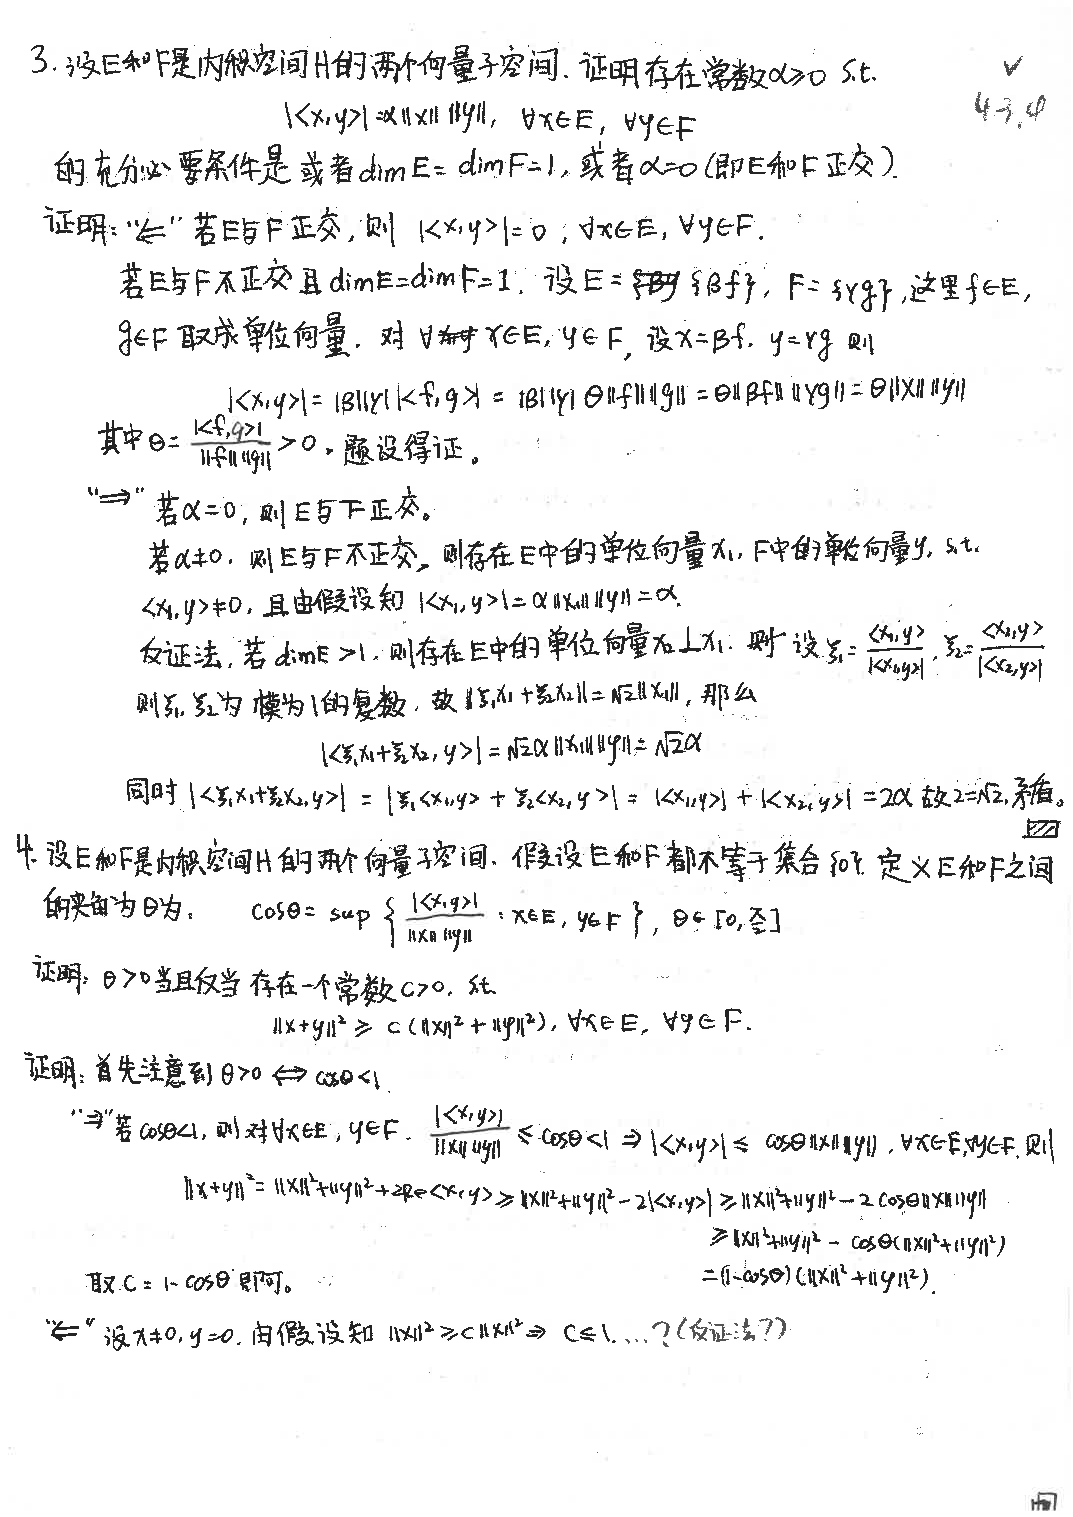
\includepdf[pages={1-1}]{4_3_4.pdf}
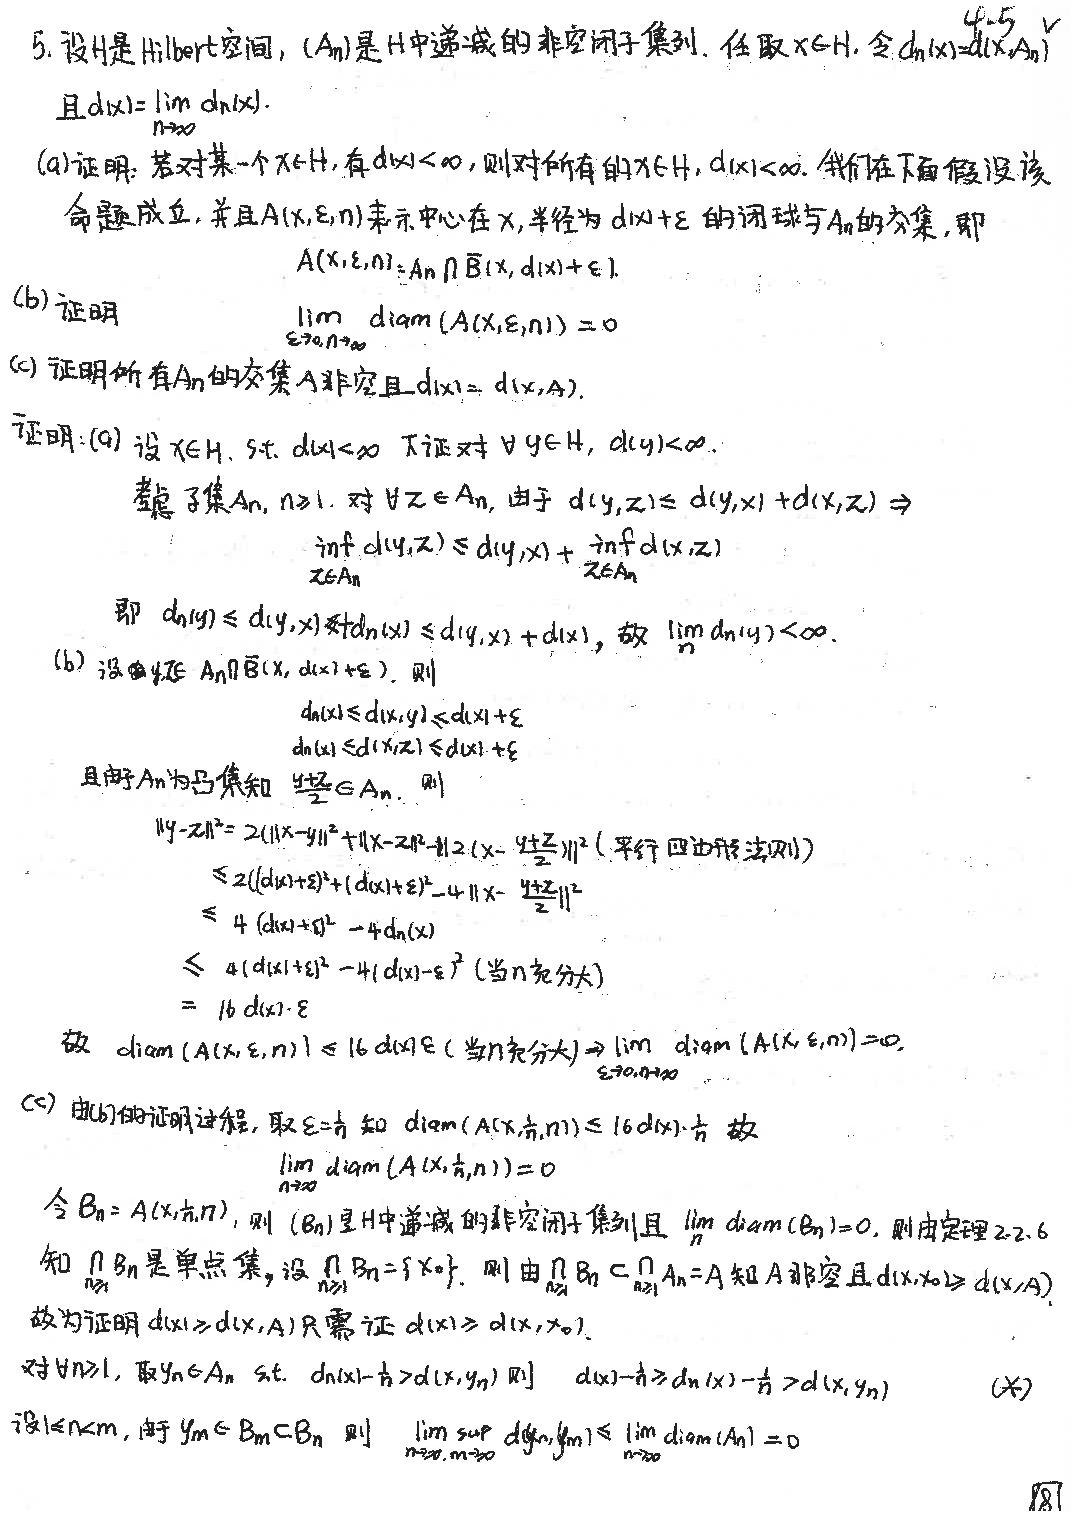
\includepdf[pages={1-1}]{4_5.pdf}
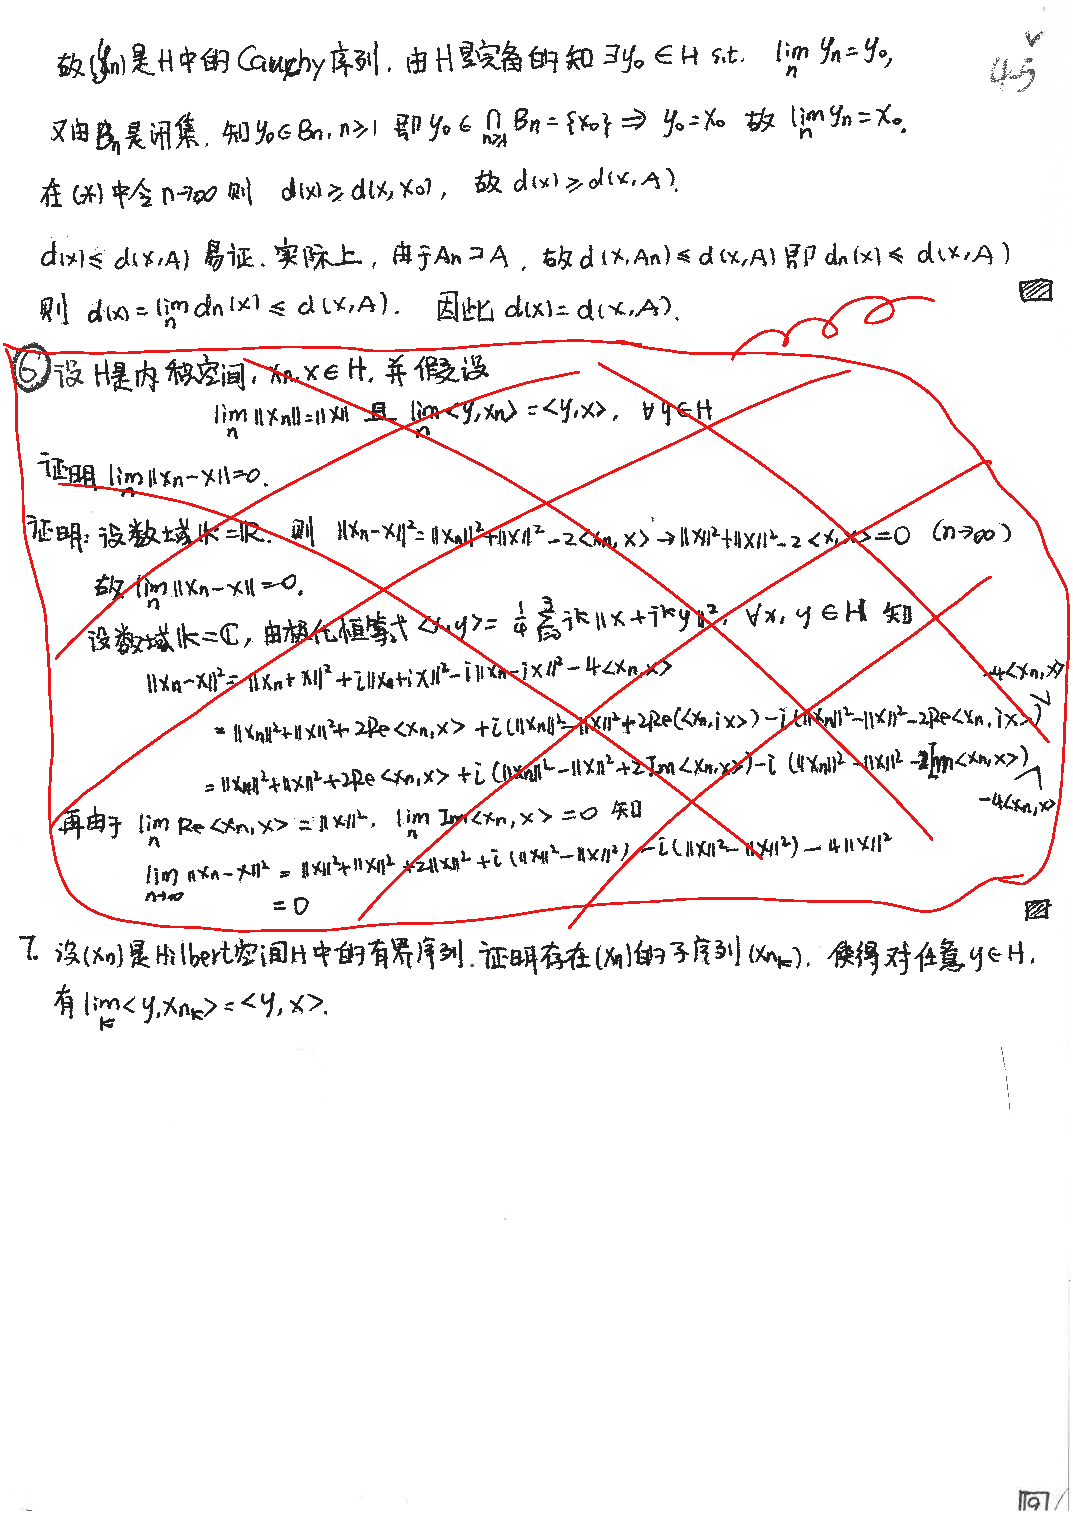
\includepdf[pages={1-1}]{4_5_1.pdf}
6. [作业]设$H$是内积空间,$x_n,x\in H$, 并假设
\begin{equation*}
	\lim_{n}\|x_n\|=\|x\|\mbox{ 且 }\lim_{n}\langle y,x_n\rangle=\la y,x\ra,\forall y\in H,
\end{equation*}
证明$\lim_n\|x_n-x\|=0$.
\begin{proof}
	设数域$\mathbb{K}=\mathbb{R}$, 则
	$$\|x_n-x\|^2=\|x_n\|^2+\|x\|^2-2\la x_n,x\ra\to \|x\|^2+\|x\|^2-2\la x,x\ra(n\to\infty),$$
	故$\lim_n\|x_n-x\|=0$.
	
	设数域$\mathbb{K}=\mathbb{C}$, 则$$\|x_n-x\|^2=\|x_n\|^2+\|x\|^2-2\mathrm{Re}\la x_n,x\ra\to \|x\|^2+\|x\|^2-2\mathrm{Re}\la x,x\ra=0(n\to\infty).$$
	故$\lim_n\|x_n-x\|=0$.
\end{proof}
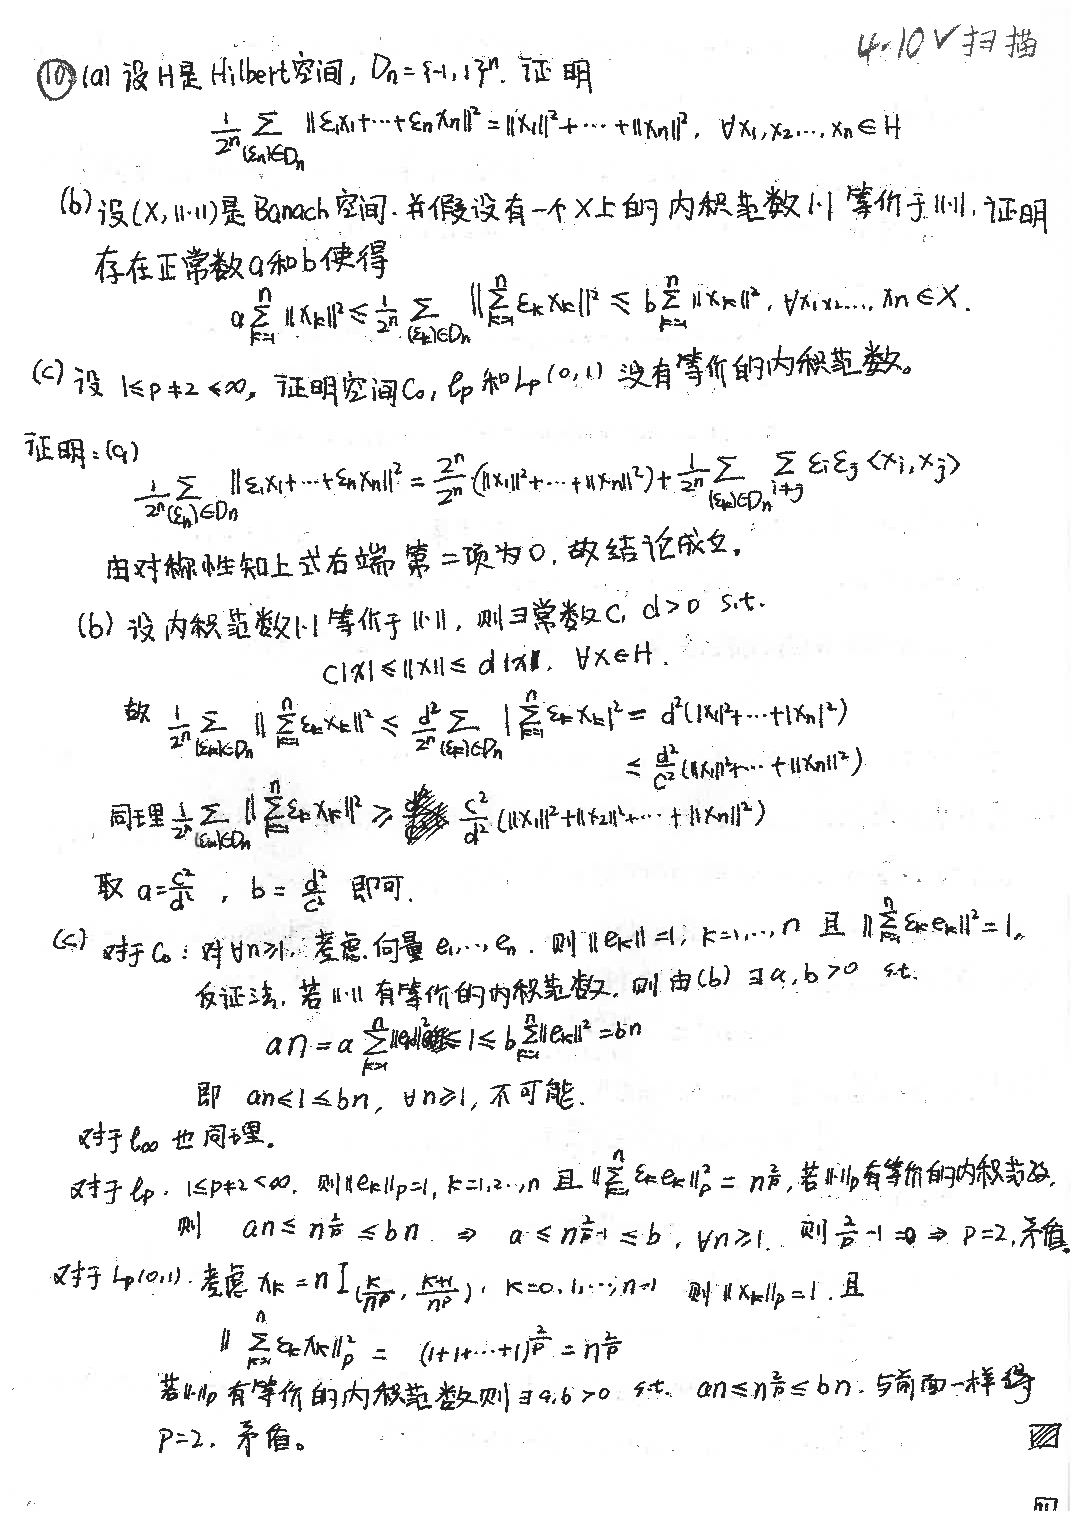
\includepdf[pages={1-1}]{4_10.pdf}

11. [作业]设$(C_n)$是Hilbert空间$H$中的一个递增的非空闭凸子集列,$C$是所有$C_n$的并集的闭包。证明:$P_C(x)=\lim_{n\to\infty}P_{C_n}(x),\forall x\in H$.
\begin{proof}
	先证$P_{C_n}(x)$依范数收敛。由于$C_n$递增则序列$(\|x-P_{C_n}(x)\|)_{n\geq 1}$单调递减有下界故收敛,则对于任意$n,m\geq 1$, 不妨设$n<m$, 则
	\begin{equation*}
	\begin{split}
	\|P_{C_n}(x)-P_{C_m}(x)\|^2=&\|P_{C_n}(x)-x-(P_{C_m}(x)-x)\|^2\\
	=&2(\|P_{C_n}(x)-x\|^2+\|P_{C_m}(x)-x\|^2)-\|P_{C_n}(x)+P_{C_m}(x)-2x\|^2\\
	=&2(\|P_{C_n}(x)-x\|^2+\|P_{C_m}(x)-x\|^2)-4\|\frac{P_{C_n}(x)+P_{C_m}(x)}{2}-x\|^2\\
	\leq &2(\|P_{C_n}(x)-x\|^2+\|P_{C_m}(x)-x\|^2)-4\|P_{C_m}(x)-x\|^2\\
	=&2(\|P_{C_n}(x)-x\|^2-\|P_{C_m}(x)-x\|^2)\to 0(n,m\to\infty),
	\end{split}
	\end{equation*}
	其中第二个等式是由于平行四边形法则,不等式是由于$\frac{P_{C_n}(x)+P_{C_m}(x)}{2}\in C_m$. 因此$(P_{C_n}(x))_{n\geq 1}$是$H$中的Cauchy列,$H$完备,故$(P_{C_n}(x))_{n\geq 1}$收敛于某个$y\in H$, 即$\lim_{n\to \infty}P_{C_n}(x)=y$. 又对于任意$n\geq 1$, 
	\begin{equation*}
	\mathrm{Re}\la x-P_{C_n}(x),z-P_{C_n}(x)\ra\leq 0, \forall z\in C_n,
	\end{equation*}
	令$n\to\infty$由内积的连续性得
	$$\mathrm{Re}\la x-y,z-y\ra\leq 0,\forall z\in C_n,\forall n\geq 1,$$
	进一步
	$$\mathrm{Re}\la x-y,z-y\ra\leq 0,\forall z\in C,$$
	故$y=P_C(x)$, 因此$P_C(x)=\lim_{n\to\infty}P_{C_n}(x)$, $\forall x\in H$.
\end{proof}

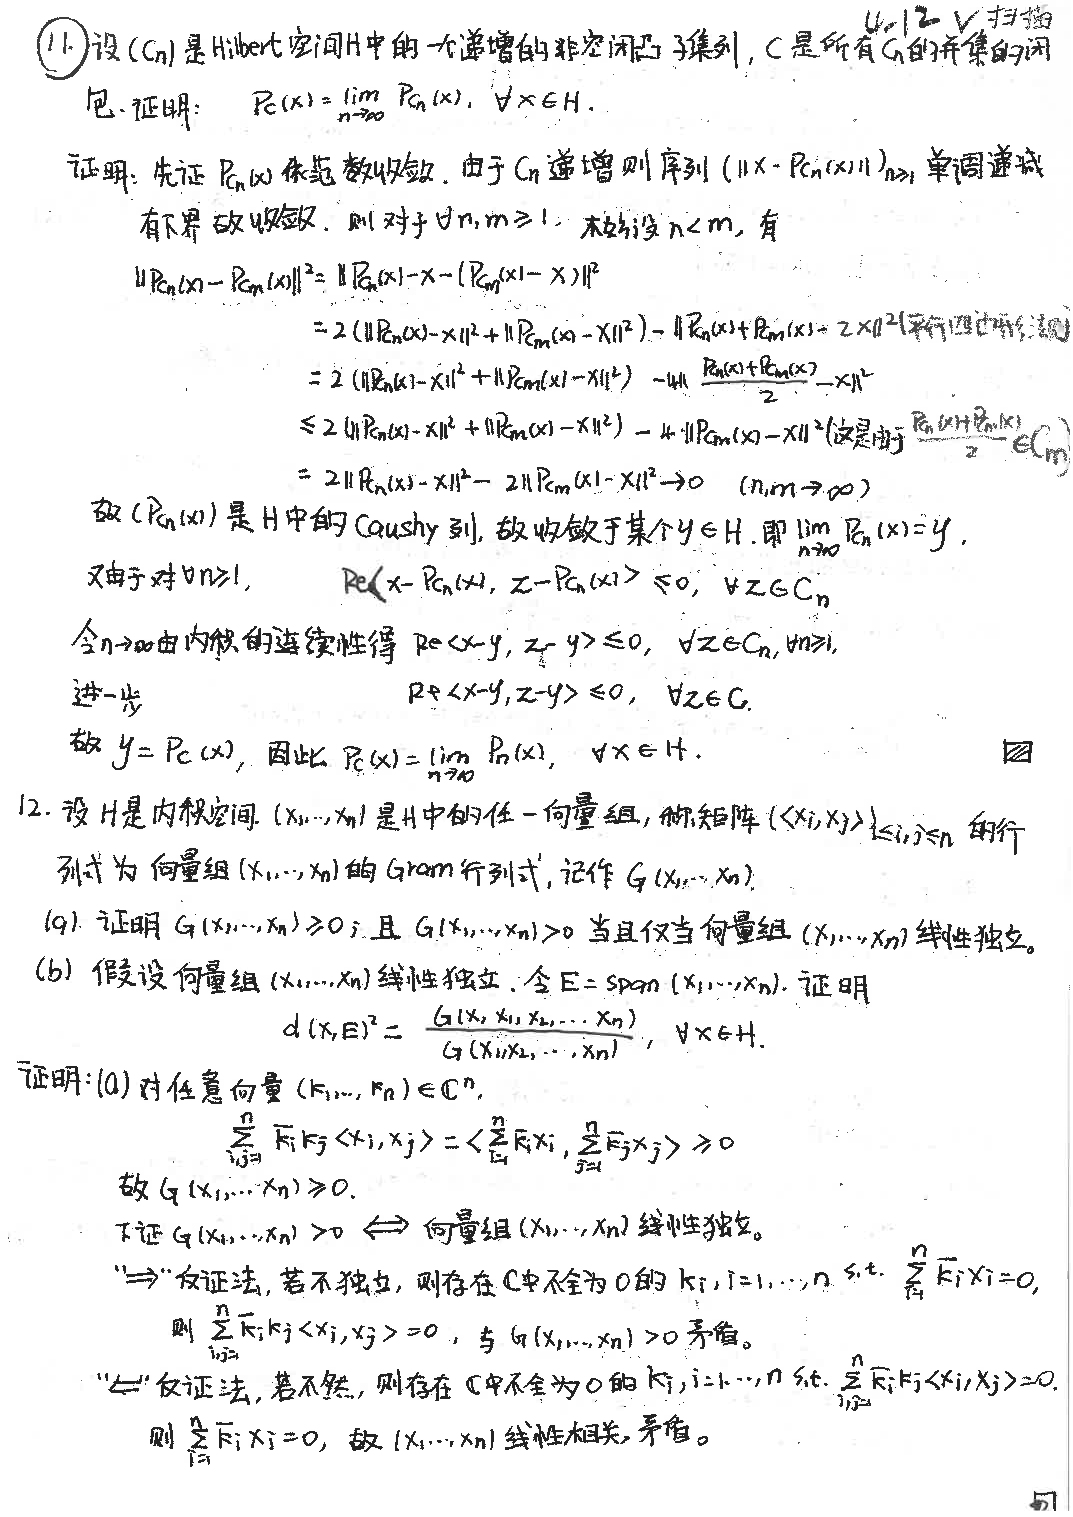
\includepdf[pages={1-1}]{4_12.pdf}
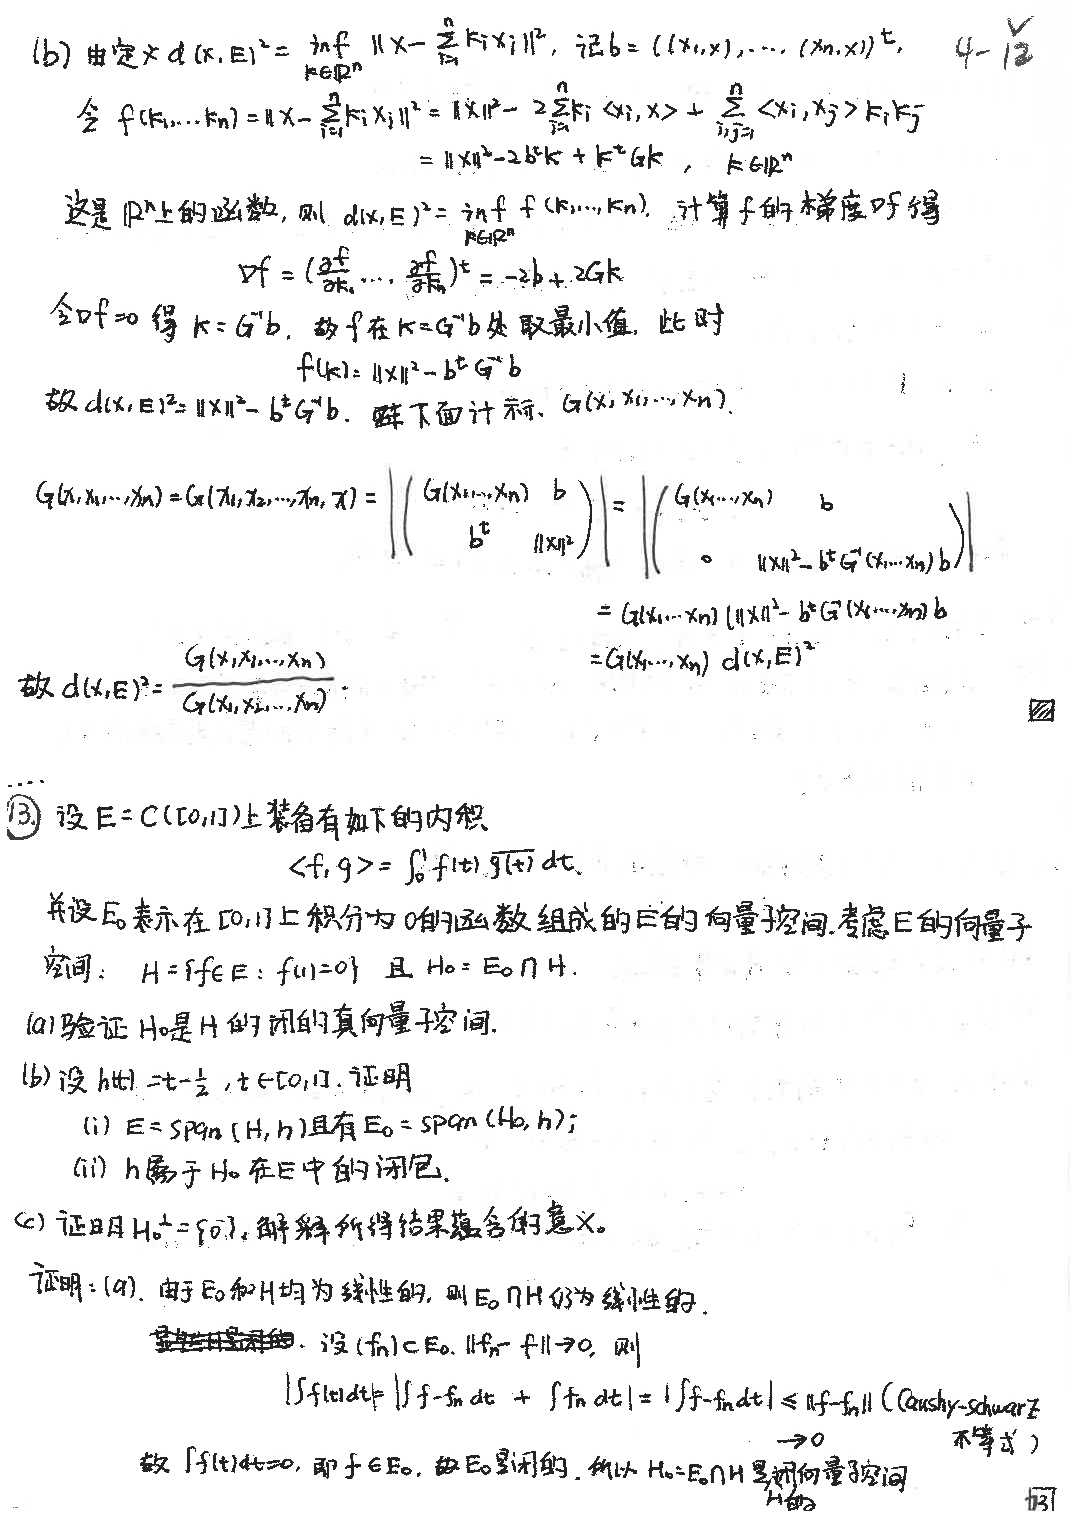
\includepdf[pages={1-1}]{4_12_1.pdf}
13. 设$E=C([0,1])$上装备有如下内积
\begin{equation*}
\la f,g\ra=\int_0^1 f(t)\overline{g(t)}dt.
\end{equation*}
并设$E_0$表示再$[0,1]$上积分为$0$的函数组成的$E$的向量子空间。考虑$E$的向量子空间: $H=\{f\in E:f(1)=0\}$且$H_0=E_0\cap H$.
\begin{enumerate}
	\item[(a)] 验证$H_0$是$H$的闭的真向量子空间。
	\item[(b)] 设$h(t)=t-\frac{1}{2},t\in[0,1]$, 证明
	\begin{enumerate}
		\item[(i)] $E=\mathrm{span}(H,h)$, 且有$E_0=\mathrm{span}(H_0,h)$;
		\item[(ii)] $h$属于$H_0$在$E$中的闭包。
	\end{enumerate}
	\item[(c)] 限制在$H$中讨论,证明$H_0^{\perp}=\{0\}$, 解释所得结果蕴含的意义。
\end{enumerate}
\begin{proof}
	(a) 由于$E_0$和$H$均为线性的,则$E_0\cap H$也是线性的。设$(f_n)\subset E_0$, $\|f_n-f\|\to 0$, 则由Cauchy-Schwarz不等式知
	\begin{equation*}
	|\int f(t)dt|=|\int f-f_ndt+\int f_ndt|=|\int f-f_ndt|\leq \|f-f_n\|_2\to 0
	\end{equation*}
	故$\int f(t)dt=0$, 即$f\in E_0$, 故$E_0$是$E$中的闭子空间,所以$H_0=E_0\cap H$是$H$中的闭向量子空间。
	
	设$f(t)=(t-1)^2$, 则$f\in H$, 但$f\notin H_0$, 故$H_0$真包含于$H$. 
	
	(b) \begin{enumerate}
		\item[(i)] 对任意$f\in E$, $f-2f(1)h\in H$, 故$E=\mathrm{span}(H,h)$.
		
		对任意$f\in E_0$, $f-2f(1)h\in H$且$f-2f(1)h\in E_0$, 故$f-2f(1)h\in H_0$, 所以$E_0=\mathrm{span}(H_0,h)$.
		
		\item[(ii)] 设$f_n$为连接$(0,0),(\frac{1}{n},h(\frac{1}{n})),(1-\frac{1}{n},h(1-\frac
		{1}{n})), (1,0)$的折线函数,则由于
		$$|h(t)-f_n(t)|\leq 1\Rightarrow |h(t)-f_n(t)|^2\leq |h(t)-f_n(t)|,\forall t\in[0,1],$$ 
		故
		\begin{equation*}
		\int_0^1|h-f_n|^2 dt\leq \int_0^1|h-f_n|dt=\frac{1}{n}\cdot\frac{1}{2}\cdot\frac{1}{2}\cdot 2=\frac{1}{2n}\to 0(n\to \infty),
		\end{equation*}
		故$\|f_n-h\|_2\to 0$, 且$f_n\in H_0$, 因此$h$属于$H_0$在$E$中的闭包。
	\end{enumerate}
	(c) 这里限制在$H$中讨论,由(b)知$E_0\subset\overline{H_0}$。任取$f\in H_0^\perp$, 则$f\perp\overline{H_0}$. 令$g=f-\int_0^1 f(t)dt$, 则$g\in E_0\subset \overline{H_0}$, 则
	\begin{equation}
	\la f,g\ra=0\Rightarrow \la f,f\ra-|\int_0^1 f(t)dt|^2=\|f\|^2-|\la f,1\ra|^2=0,
	\end{equation}
	又由Cauchy-Schwarz不等式的等式条件,这意味着存在常数$C$, s.t. $f\equiv C$, 又因为$f(1)=0$, 故$f\equiv 0$. 
	
	本题说明当所讨论的内积空间不完备时,正交分解定理不一定成立。实际上,若成立,则$H=\overline{H_0}\oplus H_0^\perp=\overline{H_0}=H_0$, 这与(a)矛盾。
\end{proof}

15. (a) 设$E$和$F$是Hilbert空间$H$的两个正交向量子空间。证明$E+F$是闭的当且仅当$E$和$F$都是闭的。

(b) $(e_n)$表示$\ell_2$中的标准正交基,设$E$是$\{e_{2n},n\geq 1\}$的线性扩张的闭包,而$F$是$\{e_{2n}+\frac{1}{n}e_{2n+1}:n\geq 1\}$的线性扩张的闭包。证明$E\cap F=\{0\}$并且$E+F$在$\ell_2$中不是闭的。
\begin{proof}
	(a) "$\Leftarrow$", 设$E$和$F$都是闭的,若有序列$(z_n)\subset E+F$, $z_n=x_n+y_n$, $x_n\in E,y_n\in F$, $z_n\to z(n\to\infty)$, 想证$z\in E+F$. 
	
	由于$\|x_n+y_n-z\|^2\to 0$, 则$\|x_n+y_n-(x_m+y_m)\|^2\to 0(n,m\to\infty)$, 故
	\begin{equation*}
	\begin{split}
	\|x_n-x_m\|^2=&\|x_n+y_n-y_n-(x_m+y_m)+y_m\|^2\\
	=&\|x_n+y_n-(x_m+y_m)-(y_n-y_m)\|^2\\
	=&\|x_n+y_n-(x_m+y_m)\|^2+\|y_n-y_m\|^2-2\mathrm{Re}\la x_n+y_n-(x_m+y_m),y_n-y_m\ra\\
	=&\|x_n+y_n-(x_m+y_m)\|^2-\|y_n-y_m\|^2
	\end{split}
	\end{equation*}
	故$\|x_n-x_m\|^2+\|y_n-y_m\|^2=\|x_n+y_n-(x_m+y_m)\|^2\to 0(n,m\to\infty)$, 这意味着$(x_n)$与$(y_n)$都是Cauchy列,因而收敛,设$x_n\to x,y_n\to y$, 则$x\in E,y\in F$, 且$x_n+y_n\to x+y$, 故$z=x+y\in E+F$, 所以$E+F$是闭的。
	
	"$\Rightarrow$", 设$E+F$是闭的。若有序列$(x_n)\subset E$, $x_n\to x$, 注意到$x_n=x_n+0\in E+F$, 而$E+F$是闭的,那么$x\in E+F$, 设$x=y+z,y\in E,z\in F$. 则
	\begin{equation*}
	\|x_n-y-z\|^2=\|x_n-y\|^2+\|z\|^2\to 0\Rightarrow \|z\|^2=0\Rightarrow z=0,
	\end{equation*}
	故$x\in E$. 所以$E$是闭的,同理可证$F$是闭的。
	
	(b) 先证明$E\cap F=\{0\}$. 由题设知$E,F$中的元素具有如下形式:
	\begin{equation*}
	\begin{split}
	x=(0,x_2,0,x_4,0,x_6,0,x_8,\cdots), \forall x\in E,\\
	y=(0,y_2,y_2,y_4,\frac{1}{2}y_4,y_6,\frac{1}{3}y_6,y_8,\cdots), \forall y\in F,
	\end{split}
	\end{equation*}
	所以,若$x=y$, 则$y_2=0,y_4=0,\cdots$, 故$y=0$, 因此$E\cap F=\{0\}$.
	
	下证$E+F$在$\ell_2$中不是闭集。取$E$中的序列$a_n=-\sum_{k=1}^n e_{2k},n\geq 1$, $F$中的序列$b_n=\sum_{k=1}^ne_{2k}+\frac{1}{k}e_{2k+1}$, 则
	$$a_n+b_n=\sum_{k=1}^n\frac{1}{k}e_{2k+1}\in E+F,$$
	且$\sum_{k=1}^n\frac{1}{k}e_{2k+1}\to \sum_{k=1}^\infty\frac{1}{k}e_{2k+1}\in\ell_2$, 若$\sum_{k=1}^\infty\frac{1}{k}e_{2k+1}\in E+F$, 则存在$x\in E,y\in F$, 使得
	\begin{equation*}
	\begin{split}
	\sum_{k=1}^\infty\frac{1}{k}e_{2k+1}=x+y=&\sum_{k=1}^\infty x_{2k}e_{2k}+\sum_{k=1}^\infty y_{2k}e_{2k}+\frac{1}{k}y_{2k}e_{2k+1}\\
	=&\sum_{k=1}^\infty (x_{2k}+y_{2k})e_{2k}+\sum_{k=1}^\infty \frac{1}{k}y_{2k}e_{2k+1},
	\end{split}	
	\end{equation*}
	这意味着
	\begin{equation*}
	\begin{cases}
	x_{2k}+y_{2k}=0\\
	\frac{1}{k}y_{2k}=\frac{1}{k}
	\end{cases}\Rightarrow 
	\begin{cases}
	x_{2k}=-1\\
	y_{2k}=1
	\end{cases}
	\Rightarrow \sum_{k=1}^\infty |x_k|^2=\infty,
	\end{equation*}
	故$x\notin E$, 矛盾,故$\sum_{k=1}^\infty \frac{1}{k}e_{2k+1}\notin E+F$, 因此$E+F$不是闭集。
\end{proof}
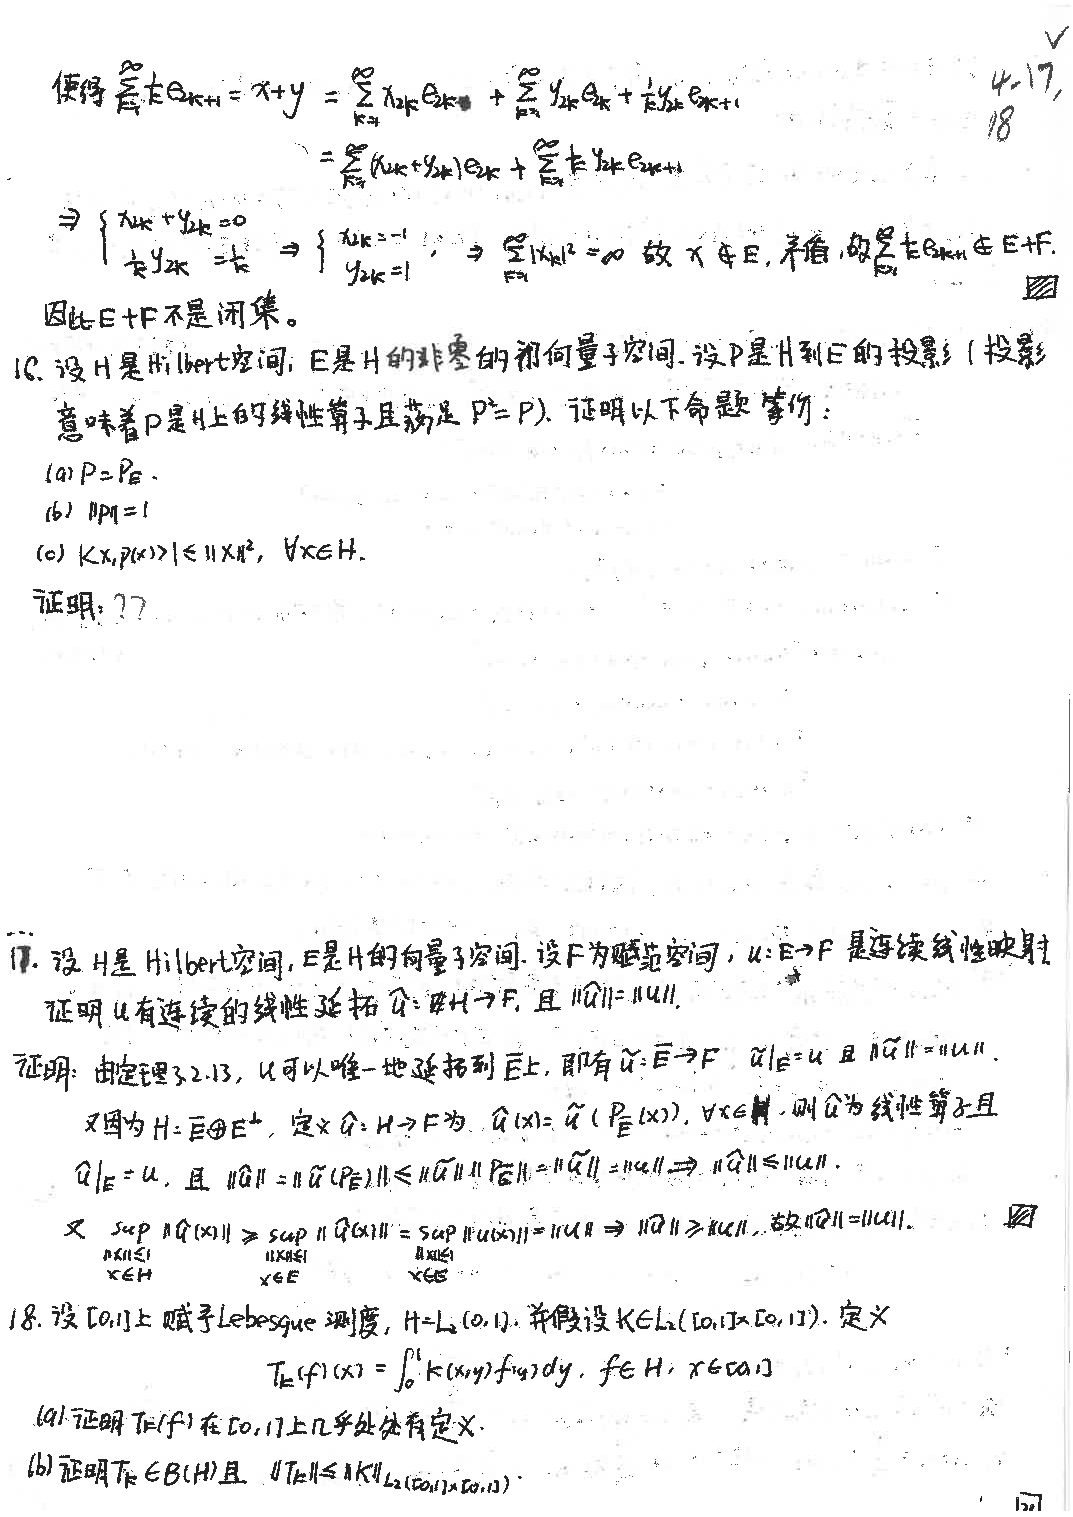
\includepdf[pages={1-1}]{4_17_18.pdf}
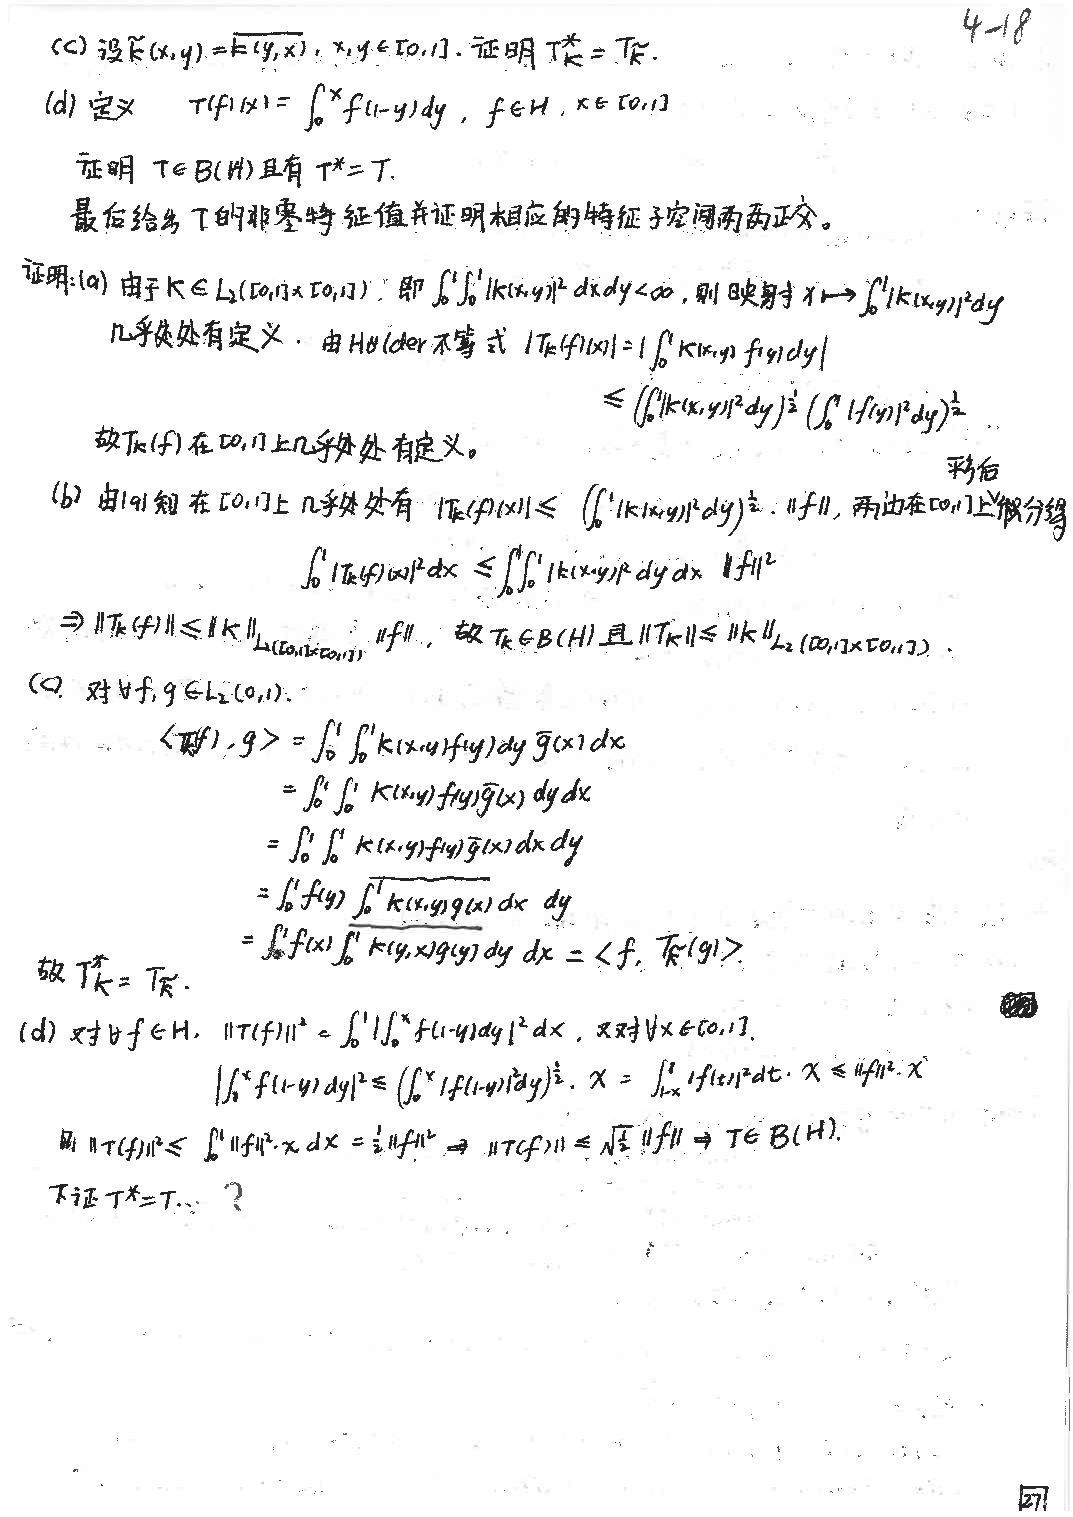
\includepdf[pages={1-1}]{4_18.pdf}
\includepdf[pages={1-1}]{4_19_21.pdf}

20. 
\begin{proof}
	
	(a)\textbf{法II}: 对于$0< t\leq r$, 由Cauchy积分公式知 $f(z)=\frac{1}{2\pi}\int_0^{2\pi}f(z+te^{i\theta})d\theta$, 故
	\begin{equation*}
	\begin{split}
	\frac{1}{\pi r^2}\int_{\overline{B}(z,r)}f(w)d\lambda(w)=\frac{1}{\pi r^2}\int_0^r\int_0^{2\pi}f(z+te^{i\theta})td\theta dt=\frac{1}{\pi r^2}\int_0^r 2\pi f(z)tdt=f(z).
	\end{split}
	\end{equation*} 
	其中第二个等式利用了Cauchy积分公式。
	
	(b) 设$z\in \Omega$, $d(z,\Omega^c)>r$, 则$\Omega^c\subset \overline{B}(z,r)^c$, 即$\overline{B}(z,r)\subset \Omega$, 故由(a)知$f(z)=\frac{1}{\pi r^2}\int_{\overline{B}(z,r)}f(w)d\lambda(w)$, 由H\"older不等式,
	\begin{equation*}
	\begin{split}
	|f(z)|=\frac{1}{\pi r^2}|\int_{\overline{B}(z,r)}f(w)d\lambda(w)|\leq &  \frac{1}{\pi r^2}[\int_{\overline{B}(z,r)}|f(w)|^2d\lambda(w)]^{\frac{1}{2}}\cdot [\int_{\overline{B}(z,r)}1 d\lambda(w)]^{\frac{1}{2}}\\
	\leq &\frac{1}{\sqrt{\pi}r}\|f\|_2.
	\end{split}
	\end{equation*}
	
	(c) 只需证明$H_\Omega$的完备性和可分性。
	
	完备性:设$(f_n)$是$H_\Omega$中的Cauchy列,由$L_2(\Omega)$完备知存在$f\in L_2(\Omega)$, 使得$\|f_n-f\|_2\to 0$, 下面只需证明$f$几乎处处等于$\Omega$上的一个解析函数。对任意$z\in \Omega$, 存在$r>0$, s.t. $d(z,\Omega^c)>r$, 则$\overline{B}(z,r)\subset \Omega$, 则由(b)知$|f_n(z)-f_m(z)|\leq \frac{1}{\sqrt{\pi}r}\|f_n-f_m\|_2$. 更进一步,由于$d(z,\Omega^c)$是关于$z$的连续函数,则存在$r_1>0$, s.t. $B(z,r_1)\subset \{z:d(z,\Omega^c)>r\}$, 则
	\begin{equation*}
	|f_n(w)-f_m(w)|\leq \frac{1}{\sqrt{\pi}r}\|f_n-f_m\|_2, \forall w\in B(z,r_1),
	\end{equation*}
	故$(f_n(w))$是$\mathbb{C}$中的Cauchy列,则必收敛,设$g(w)=\lim_{n}f_n(w)$, 在上式中令$m\to\infty$则
	\begin{equation*}
	|f_n(w)-g(w)|\leq \frac{1}{\sqrt{\pi}r}\|f_n-f\|_2, \forall w\in B(z,r_1),
	\end{equation*}
	故$(f_n)$在$B(z,r_1)$上一致收敛于$g$, 所以$g$在$B(z,r_1)$上解析(参见p94). 这样在$\Omega$的任意点$z\in \Omega$附近都能找到一个开球,这个开球内存在一个解析函数是$(f_n)$的$L_2$极限,取遍$\Omega$所有点时,这些开球覆盖整个$\Omega$, 定义$\Omega$上的一个函数在上述每个开球内的取值等于我们找到的函数$g$, 则由定义知该函数是良定义的,且是解析的。再由Fatou引理,
	\begin{equation*}
	\int_\Omega|f(w)-g(w)|^2\leq \liminf_{n\to\infty}\int_\Omega|f(w)-f_n(w)|^2d\lambda(w)=0,
	\end{equation*}
	故$f=g$, 几乎处处,所以$(f_n)$依$L_2$范数收敛于解析函数$g$, 故$H_\Omega$完备。
	
	可分性:可分度量空间的子空间仍然是可分的, $H_\Omega\subset L_2(\Omega)$, 所以$H_\Omega$是可分的。
	
	(d) 设$z\in\Omega$, 则存在$r>0$, s.t. $d(z,\Omega^c)>r$, 由(b)知$|f(z)|\leq \frac{1}{\sqrt{\pi}r}\|f\|_2$, 则
	\begin{equation*}
	|\delta_z(f)=|f(z)|\leq \frac{1}{\sqrt{\pi}r}\|f\|_2,\forall f\in H_\Omega,
	\end{equation*} 
	故$\delta_z$是$H_\Omega$上的连续线性泛函,由Riesz表示定理得,存在$K_z\in H_\Omega$, 使得
	$$f(z)=\int_\Omega f(w)\overline{K_z(w)}d\lambda(w),\forall f\in H_\Omega.$$
	
	(e) (i) 由(d)知 
	$$f(z)=\la f,K_z\ra,\forall f\in H_\Omega, \forall z\in\Omega,$$
	取$f=K_w$则
	$$K_w(z)=\la K_w,K_z\ra=\overline{\la K_z,K_w\ra}=\overline{K_z(w)},$$
	故$K_\Omega(z,w)=\overline{K_\Omega(w,z)}$.
	
	(ii) 给定一组$H_\Omega$中的标准正交基$(e_n)_{n\geq 1}$, 则
	$$K_z=\sum_{n=1}^\infty\la K_z,e_n\ra e_n=\sum_{n=1}^\infty \overline{\la e_n,K_z\ra}e_n=\sum_{n=1}^\infty \overline{e_n(z)}e_n,$$
	且由Parseval恒等式知上式在$H_\Omega$中收敛。
	
	(f) (i)$e_n(z)=\sqrt{\frac{n+1}{\pi}}z^n$, $n\geq 0$, 计算$\la e_n,e_m\ra$得
	$$\la e_n,e_m\ra=\frac{\sqrt{(n+1)(m+1)}}{\pi}\int_0^{2\pi}\int_0^1 r^{n+m}e^{i(n-m)\theta}rdr d\theta=\delta_{n,m},$$
	故$(e_n)$规范正交. 对任意$f\in H_\Omega$, 设$f$的Taylor展为$\sum_{n=0}^{\infty}a_nz^n$(在任何紧子集上一致收敛), 则
	\[
	f(z)=\sum_{n=0}^{\infty} a_nz^n=\sum_{n=0}^{\infty}\frac{a_n\sqrt{\pi}}{\sqrt{n+1}}e_n(z)=\sum_{n=0}^{\infty} b_ne_n(z),\forall z\in D
	\]
	其中$b_n=\frac{a_n\sqrt{\pi}}{\sqrt{n+1}}$. 对任意固定的$r\in[0,1)$, $f(z)=\sum_{n=0}^{\infty} a_nr^ne^{in\theta}$在$\theta\in [0,2\pi)$上一致收敛,则在$L_2([0,2\pi))$中收敛,由Parseval恒等式知
	\[
	\int_0^{2\pi} |f(re^{i\theta})|^2\, d\theta=\int_0^{2\pi}|\sum_{n=0}^{\infty}a_nr^ne^{in\theta}|^2\, d\theta=2\pi\sum_{n=0}^{\infty}|a_n|^2r^{2n}
	\]
	则%%\int_{[0,1]*[0,2\pi)}=\int_{[0,1)*[0,2\pi)}因为$f$是$L_2$可积,且左右积分区域只相差一个零测集
	\[\begin{split}
	\int_{D}|f(\omega)|^2\, d\lambda(\omega) &= \int_0^1 \int_0^{2\pi} |f(re^{i\theta})|^2\, d\theta \, r\, dr = \int_0^12\pi\sum_{n=0}^{\infty}|a_n|^2r^{2n}\, r\, dr\\
	&=2\pi \sum_{n=0}^{\infty}|a_n|^2/(2n+2)=\sum_{n=0}^{\infty}|b_n|^2,
	\end{split}
	\]
	其中第三个等式是由于单调收敛定理,则$\sum_{n=0}^{\infty}|b_n|^2<\infty$, 故
	\[
	\|f-\sum_{k=0}^nb_ke_k(z)\|^2=\sum_{k=n+1}^{\infty}|b_k|^2\to 0\ (n\to\infty),
	\]
	故$(e_n)$是$H_D$的规范正交基。
	
	(ii) 由(e)知
	\begin{equation*}
	\begin{split}
	K_D(w,z)=\la K_z,K_w\ra=&\sum_{n=0}^\infty \overline{e_n(z)}e_n(w)\\
	=&\sum_{n=0}^\infty\frac{n+1}{\pi}\overline{z}^nw^n=\sum_{n=0}^\infty\frac{n+1}{\pi}(\overline{z}w)^n=\frac{1}{\pi}\sum_{n=0}^\infty (n+1)t^n=\frac{1}{\pi}(\sum_{n=0}^\infty t^{n+1})'\\
	=&\frac{1}{\pi}\left(\frac{t}{1-t}\right)'=\frac{1}{\pi}\frac{1}{(1-t)^2}=\frac{1}{\pi}\frac{1}{(1-\overline{z}w)^2}.
	\end{split}
	\end{equation*}
	其中$t=\overline{z}w$. 
\end{proof}



\section{第五章 习题}
1. [习题课]对任意$x\in[0,1]$, 设$f_n(x)=x^n$. 在$[0,1]$上的哪些点处,$(f_n)_{n\geq 1}$等度连续?
\begin{proof}
	当$x\in[0,1)$时,$(f_n)_{n\geq 1}$等度连续,在$x=1$处,不等度连续。
	
	实际上,设$a\in[0,1)$, 注意到
	\[\begin{split}
	|x^n-a^n|=|(x-a)(x^{n-1}+x^{n-2}a+\cdots+a^{n-1})|\leq& (1+a+\cdots+a^{n-1})|x-a|\\
	=&\frac{1-a^n}{1-a}|x-a|<\frac{1}{1-a}|x-a|,
	\end{split}
	\]
	故$(f_n)_{n\geq 1}$等度连续。	
	当$a=1$时,对$1$的任何去心邻域内任意点$x$, $|f_n(x)-f_n(1)|\to 1(n\to\infty)$, 取$\e=1/2$, 存在$n$, s.t. $|f_n(x)-f_n(1)|>1/2$, 所以在$x=1$处不等度连续
\end{proof}

2. [作业]设$K$是度量空间,$E$是赋范空间,$(f_n)_{n\geq 1}$是一列从$K$到$E$的连续函数。证明若$(f_n)_{n\geq 1}$在一点$x$处等度连续,则对任一收敛到$x$的点列$(x_n)_{n\geq 1}$, 都有$(f_n(x)-f_n(x_n))_{n\geq 1}$收敛到0. 进而证明如果$(f_n(x))_{n\geq 1}$在$E$中收敛到$y$, 那么对任一收敛到$x$的点列$(x_n)_{n\geq 1}$, $(f_n(x_n))_{n\geq 1}$也收敛到$y$. \\
取$f_n(x)=\sin(nx)$. 证明$(f_n)_{n\geq 1}$在$\mathbb{R}$上每一点都不等度连续。
\begin{proof}
	设$(f_n)_{n\geq 1}$在$x$处等度连续,即对任意$\e>0$, 存在$\delta$, 使得对任意$n\geq 1$, 
	\[\mbox{当} d(y,x)<\delta \mbox{时}, |f_n(y)-f_n(x)|<\e.\]
	设$x_n\to x$, 则存在$N\in\mathbb{N}$, 当$n>N$时, $d(x_n,x)<\delta$, 所以当$n>N$时,$|f_n(x_n)-f_n(x)|<\e$, 故$(f_n(x)-f_n(x_n))_{n\geq 1}$收敛到0.
	
	进一步,设$(f_n(x))_{n\geq 1}$收敛到$y$, 那么
	$$|f_n(x_n)-y|\leq |f_n(x_n)-f_n(x)|+|f_n(x)-y|\to 0,$$
	故$(f_n(x_n))_{n\geq 1}$收敛到$y$.
	
	考虑$f_n(x)=\sin(nx)$, 当$x\notin\{m\pi, m\in\mathbb{Z}\}$时, 设$x_n=x+\frac{\pi}{n}$, 则$x_n\to x$, 同时
	$$|f_n(x)-f_n(x_n)|=|\sin(nx)-(-\sin(nx))|=2|\sin (nx)|\nrightarrow0,$$
	这是因为若$\sin(nx)$收敛到$0$, 则
	\[\lim_{n\to\infty} 2\sin(x)\cos(nx)=\lim_{n\to\infty}\sin(n+1)x-\sin(n-1)x=0,\]
	又$\sin x\ne 0$, 则$\lim_{n\to\infty}\cos(nx)=0$, 又由由$\sin^2 nx+\cos^2 nx=1$知$\lim_{n\to\infty}\sin^2 nx+\lim_{n\to\infty}\cos^2 nx=1$, 矛盾,故$\sin(nx)$不可能收敛到$0$.
	所以$(f_n(x)-f_n(x_n))_{n\geq 1}$不会收敛到0, 所以$(f_n)_{n\geq 1}$在$x\notin\{m\pi, m\in\mathbb{Z}\}$处不等度连续。
	
	当$x\in\{m\pi, m\in\mathbb{Z}\}$时,取$x_n=x+\frac{\pi}{2n}$, 那么$x_n\to x$, 同时
	$$|f_n(x)-f_n(x_n)|=1\nrightarrow0,$$
	所以$(f_n)_{n\geq 1}$在$x\in\{m\pi, m\in\mathbb{Z}\}$时不等度连续。
\end{proof}
\begin{Remark}
	实际上当$x\notin\{m\pi, m\in\mathbb{Z}\}$时,$(\sin nx)$不收敛于任何数。反证法,假设$(\sin nx)$收敛,则$(\sin(n+1)x)$收敛,又
	$$\sin(n+1)x=\sin nx\cos x+\cos nx\sin x,$$
	故$(\cos nx)$收敛,设$\alpha=\lim_{n}\sin nx$, $\beta=\lim_n\cos nx$, 由$\sin^2 nx+\cos^2 nx=1$知$\alpha^2+\beta^2=1$, 故$\alpha,\beta$不能同时为$0$, 在下式
	\begin{equation*}
	\begin{cases}
	\sin(n+1)x=\sin nx\cos x+\cos nx\sin x\\
	\cos(n+1)x=\cos nx\cos x-\sin nx\sin x
	\end{cases}
	\end{equation*}
	中令$n\to\infty$得
	\begin{equation*}
	\begin{cases}
	\alpha=\alpha\cos x+\beta\sin x\\
	\beta=\beta\cos x-\alpha\sin x
	\end{cases}
	\end{equation*}
	即
	\begin{equation*}
	\begin{cases}
	(\cos x-1)\alpha+\beta\sin x=0\\
	-\alpha\sin x+(\cos x-1)\beta=0
	\end{cases}
	\end{equation*}
	有非零解,则
	\begin{equation*}
	\begin{vmatrix}
	\cos x-1 & \sin x\\-\sin x & \cos x-1
	\end{vmatrix}=0,
	\end{equation*}
	即$\cos x=1$, 这意味着$x=2k\pi,k\in \mathbb{Z}$, 矛盾,因此,$(\sin nx)$不收敛。
\end{Remark}

3.[待查] 设$K$是拓扑空间,$(E,d)$是度量空间。证明:若$(f_n)$在$C(K,E)$中依一致范数收敛,则$(f_n)$等度连续。
\begin{proof}
	设$(f_n)$收敛到$f\in C(K,E)$, 则对任意$\e>0$, 存在$N\in \mathbb{N}$, 当$n>N$时,$$\|f_n-f\|_\infty<\frac{\e}{3}.$$ 
	对任意$x\in K$, 由$f$的连续性,存在$U\in\mathcal{N}(x)$, 当$y\in U$时,$d(f(y),f(x))<\frac{\e}{3}$, 则
	\[d(f_n(y),f_n(x))\leq d(f_n(y),f(y))+d(f(y),f(x))+d(f(x),f_n(x))<\frac{\e}{3}+\frac{\e}{3}+\frac{\e}{3}=\e,
	\] 
	所以$(f_n)_{n>N}$在$x$等度连续,又因为$f_1,\cdots,f_N$是有限个连续函数,所以$(f_n)$等度连续。
\end{proof}


4.[待查] 设$K$是拓扑空间,$(E,d)$是度量空间,$(f_n)$是$C(K,E)$上等度连续序列。证明所有使得$(f_n(x))$是Cauchy序列的点$x$构成的集合是$K$中的闭子集。
\begin{proof}
	设$(x_l)$是$K$中收敛于$x$的一个序列,且每个$x_l$使得$(f_n(x_l))$是$E$中的Cauchy列。由$(f_n)$等度连续,对任意$\e>0$, 存在$U\in\mathcal{N}(x)$, 当$y\in U$时,
	$$d(f_n(y),f_n(x))<\e,$$
	又由于$x_l\to x$, 则存在$N$, 当$l\geq N$时,$x_l\in U$. 由三角形不等式,
	\[d(f_n(x),f_m(x))\leq d(f_n(x),f_n(x_N))+d(f_n(x_N),f_m(x_N))+d(f_m(x_N),f_m(x)),\]
	则上式右边的第一项和第三项小于$\e$, 又因为$(f_n(x_N))_{n\geq 1}$是Cauchy列,则存在$N_1\in\mathbb{N}$, 当$n,m>N_1$时,第二项小于$\e$, 所以当$n,m>N_1$时,
	$$d(f_n(x),f_m(x))<3\e,$$
	故$(f_n(x))$是Cauchy列,得证。
\end{proof}

5. [习题课]考虑函数序列$(f_n)_{n\geq 1}$, 这里$f_n(t)=\sin(\sqrt{t+4(n\pi)^2})$, $t\in[0,\infty)$.
\begin{enumerate}
	\item[(a)] 证明$(f_n)$等度连续并且逐点收敛到0函数。
	\item[(b)] $C_b([0,\infty),\mathbb{R})$表示$[0,\infty)$上所有有界连续函数构成的空间,并赋予范数
	$$\|f\|_\infty=\sup_{t\geq 0}|f(t)|.$$
	$(f_n)$在$C_b([0,\infty),\mathbb{R})$上是否相对紧?
\end{enumerate}
\begin{proof}
	(a) 由Lagrange中值定理,对任意$s,t\in [0,\infty)$
	\begin{equation*}
	\begin{split}
	|f_n(s)-f_n(t)|=&|\sin\sqrt{s+4(n\pi)^2}-\sin\sqrt{t+4(n\pi)^2}|\\
	=&|\frac{\cos\sqrt{\xi+4(n\pi)^2}}{2\sqrt{\xi+4(n\pi)^2}}||s-t|\leq \frac{1}{4\pi}|s-t|
	\end{split}
	\end{equation*}
	(其中$\xi\in (s,t)$)故$(f_n)$是等度连续的。
	
	注意到
	\begin{equation*}
	\sin\sqrt{t+4(n\pi)^2}=\sin(\sqrt{t+4(n\pi)^2}-2n\pi+2n\pi)=\sin(\frac{t}{\sqrt{t+4(n\pi)^2}+2n\pi})\to 0(n\to\infty),
	\end{equation*}
	所以$(f_n)$逐点收敛到0函数。
	
	(b) 不是相对紧的。反证法,若$(f_n)$相对紧,则闭包$\overline{(f_n)}$紧,由定理2.5.1, 存在子列$(f_{n_k})$收敛于某个$f\in C([0,\infty),\mathbb{R})$, 即$\|f_{n_k}-f\|_\infty\to0(k\to\infty)$, 则对任意$t\in[0,\infty)$, $f_{n_k}(t)\to f(t)(k\to\infty)$, 再由(a)知$f\equiv0$, 则子列$(f_{n_k})$一致收敛到0函数。下证这会导出矛盾,由(1)的证明过程知
	\begin{equation*}
	f_{n_k}(t)=\sin\sqrt{t+4(n_k\pi)^2}=\sin(\frac{t}{\sqrt{t+4(n_k\pi)^2}+2n_k\pi}),
	\end{equation*}
	注意到$\left|\frac{t}{\sqrt{t+4(n_k\pi)^2}+2n_k\pi}\right|\leq 1$, 所以对任意$\e>0$, $$\left|\sin(\frac{t}{\sqrt{t+4(n_k\pi)^2}+2n_k\pi})\right|<\e\Leftrightarrow\left|\frac{t}{\sqrt{t+4(n_k\pi)^2}+2n_k\pi}\right|< \arcsin(\e),$$
	取$\e=\frac{1}{2}$, 若$|f_{n_k}(t)|<1/2$, 则
	\begin{equation}\label{5.5}
	\left|\frac{t}{\sqrt{t+4(n_k\pi)^2}+2n_k\pi}\right|\leq \arcsin(\frac{1}{2})=\frac{\pi}{6}
	\end{equation}
	设$\theta=\frac{\pi}{6}$, 则上式等价于
	\begin{equation*}
	\begin{split}
	&t-2n_k\pi \theta\leq\theta \sqrt{t+4(n_k\pi)^2}\\
	&\Leftrightarrow t-2n_k\pi \theta\leq 0\mbox{ 或 }\\
	&t-2n_k\pi \theta\geq 0\mbox{ 且 }(t-2n_k\pi \theta)^2\leq \theta^2(t+4(n_k\pi)^2)
	\end{split}
	\end{equation*}
	后者等价于
	\begin{equation*}
	2n_k\pi \theta \leq t\leq 4n_k\pi\theta+\theta^2,
	\end{equation*}
	故式(\ref{5.5})等价于$t\leq 4n_k\pi\theta+\theta^2$, 这意味着$(f_{n_k})$不可能一致收敛于0函数,因此$(f_n)$在$C_b([0,\infty),\mathbb{R})$上不是相对紧的。
\end{proof}
\begin{Remark}
	本题说明了在定理5.1.4, 定理5.1.6中去掉$K$的紧性后,结论不再成立。
\end{Remark}

7. 本习题的目的是在Ascoli定理中的空间$(K,\delta)$是紧度量空间时,给充分性部分一个简单的证明。\\
设$(K,\delta)$是紧度量空间,$(f_n)\subset C(K,E)$是等度连续的函数列,并且对每个点$x\in K$, $\{f_n(x):n\geq 1\}$相对紧。
\begin{enumerate}
	\item[(a)] 证明$K$是可分的,即存在一个可数子集$D$在$K$中稠密。
	\item[(b)] 使用对角线法,证明$(f_n)$有一个子列$(f_{n_k})_k$, 使得对任意$x\in D$, $(f_{n_k}(x))_k$收敛。
	\item[(c)] 证明对任意$x\in K$, $(f_{n_k}(x))_k$是Cauchy序列;并由此导出$(f_{n_k})_k$在$C(K,E)$中收敛。
\end{enumerate}
\begin{proof}
	(a) 对任意有理数$r\in Q$, 由$(K,\delta)$的紧性知存在有限个$K$中的元素$x_1^r,\cdots,x_{n_r}^r$使得$$K=\cup_{k=1}^{n_r}B(x_k^r,r)=\cap_{r\in Q}\cup_{k=1}^{n_r}B(x_k^r,r).$$
	设$D=\{x_k^r,k=1,2,\cdots,n_r, r\in Q\}$, 上式意味着可数子集$D$在$K$中稠密,所以$K$是可分的。
	
	(b) 设$D=(x_m)$, 由已知条件知$(f_n(x_1))_{n\geq 1}$相对紧,因此存在子列$(f_{1,k}(x_1))_{k\geq 1}$收敛。显然对任意$x\in K$, 子列$(f_{1,k}(x))_k$仍然相对紧,则对于$x_2$, 存在子列$(f_{2,k}(x_2))_k$收敛,$\cdots$, 依此类推得到一系列收敛列$(f_{m,k}(x_m))_k,m=1,2,\cdots$. 由对角线法则,取函数序列$(f_{k,k})$, 那么对任意$x_m\in D$, $(f_{k,k}(x_m))$收敛。
	
	(c) 由$(f_n)$等度连续,则任意$\e>0$, 存在$\eta>0$, 当$\delta(x,y)<\eta$时,
	$$d(f_n(x),f_n(y))<\e,$$
	由(a)知对任意$x\in K$, 存在$x_m\in D$, s.t.$\delta(x,x_m)<\eta$, 则
	\begin{equation*}
	\begin{split}
	d(f_{s,s}(x),f_{t,t}(x))\leq & d(f_{s,s}(x),f_{s,s}(x_m))+d(f_{s,s}(x_m),f_{t,t}(x_m))+d(f_{t,t}(x_m),f_{t,t}(x))\\
	<&\e+d(f_{s,s}(x_m),f_{t,t}(x_m))+\e,
	\end{split}
	\end{equation*} 
	又由于$(f_{k,k}(x_m))_k$收敛,存在$N\in\mathbb{N}$, 当$s,t> N$时$d(f_{s,s}(x_m),f_{t,t}(x_m))<\e$, 代入上式得
	$$d(f_{s,s}(x),f_{t,t}(x))<3\e,$$
	故$(f_{k,k}(x))_k$是Cauchy列,再加上相对紧性知$(f_{k,k}(x))_k$收敛,则由定理5.1.4知$(f_{k,k})_k$在$C(K,E)$中收敛。
\end{proof}

8.[待查] 设$\Omega$是$\mathbb{R}^n$中得开集。给定一个紧子集$K\subset \Omega$, 对任意$f\in C(\Omega,\mathbb{C})$, 令
$$\|f\|_{\infty,K}=\sup_{x\in K}|f(x)|.$$
定义$\tau_c$为$C(\Omega,\mathbb{C})$上的集族,$\tau_c$中的元素可表示为如下形式集合的并集:
$$B_K(f,r)=\{g\in C(\Omega,\mathbb{C}):\|g-f\|_{\infty,K}<r\},$$
这里$f\in C(\Omega,\mathbb{C})$, $K\subset\Omega$是紧的且$r>0$. 
\begin{enumerate}
	\item[(a)] 证明$\tau_c$是$C(\Omega,\mathbb{C})$上的Hausdorf拓扑,称其为在$\Omega$的任一紧子集上一致收敛的拓扑。
	\item[(b)] 令$(f_n)\subset C(\Omega,\mathbb{C})$. 证明$f_n$在$\Omega$的任一紧子集上一致收敛到$f$当且仅当$f_n$依拓扑$\tau_c$收敛到$f$.
\end{enumerate}
\begin{proof}
	(a) 先证$\tau_c$是$C(\Omega,\mathbb{C})$上的拓扑:
	\begin{itemize}
		\item 任取$x\in \Omega$, 注意到$\{x\}$是紧集,则任意$f\in C(\Omega,\mathbb{C})$满足$f\in B_{x}(f,1)$, 因此
		$$C(\Omega,\mathbb{C})=\cup_{f}B_{x}(f,1).$$
		\item 显然$\tau_c$对无穷并封闭。
		\item 考虑如下两个集合:
		\begin{equation*}
			B_{k_1}(f_1,r_1)=\{g\in C(\Omega,\mathbb{C}):\|g-f_1\|_{\infty,K_1}<r_1\},
		\end{equation*}
		$$B_{k_2}(f_2,r_2)=\{g\in C(\Omega,\mathbb{C}):\|g-f_2\|_{\infty,K_2}<r_2\},$$
		设$r_3=\min\{r_1,r_2\}/2$, 对任意$g\in B_{k_1}(f_1,r_1)\cap B_{k_1}(f_1,r_1)$, 下证
		$$B_{K_1\cup K_2}(g,r_3)\subset B_{k_1}(f_1,r_1)\cap B_{k_2}(f_2,r_2).$$
		实际上,对任意$h\in B_{K_1\cup K_2}(g,r_3)$, 
		\begin{equation*}
		\begin{split}
		\|h-f_1\|_{\infty,K_1}\leq \|h-g\|_{\infty,K_1}+\|g-f_1\|_{\infty,K_1}\leq& \|h-g\|_{\infty,K_1\cup K_2}+\|g-f\|_{\infty,K_1}\\
		<&\frac{r_1}{2}+\frac{r_1}{2}=r_1,
		\end{split}
		\end{equation*}
		因此$B_{K_1\cup K_2}(g,r_3)\subset B_{k_1}(f_1,r_1)$, 同理$B_{K_1\cup K_2}(g,r_3)\subset B_{k_2}(f_2,r_2)$, 所以$\tau_c$对有限交封闭。
	\end{itemize}
    故$\tau_c$是$C(\Omega,\mathbb{C})$上的拓扑。
    
    设$f,g\in C(\Omega,\mathbb{C})$且$f\ne g$, 则存在$x_0\in \Omega$, s.t. $f(x_0)\ne g(x_0)$, 设$r_0=|f(x_0)-g(x_0)|/2$, 则$f\in B_{x_0}(f,r_0),g\in B_{x_0}(g,r_0)$且
    $$B_{x_0}(f,r_0)\cap B_{x_0}(g,r_0)=\varnothing,$$
    故$\tau_c$是Hausfdorff拓扑。
    
    (b) $\Rightarrow$: 对$f$的任何开邻域$U$, 存在紧集$K$, 半径$r>0$, s.t. $B_{K}(f,r)\subset U$, 由假设知存在$N\in\mathbb{N}$, 当$n>N$时,$f_n\in B_K(f,r)\subset U$, 故$f_n$依拓扑$\tau_c$收敛到$f$.
    
    $\Leftarrow$: 对$\Omega$的任意紧子集$K$, 任意$r>0$, 由于$B_K(f,r)\in \tau_c$, 由收敛性定义知$f_n$在$K$上一致收敛到$f$. 
\end{proof}

9.[待查] 设$\Omega$是$\mathbb{C}$中开集,$\mathcal{H}(\Omega)$表示$\Omega$上所有全纯函数构成的集合。
\begin{enumerate}
	\item[(a)] 证明对每一个紧子集$K\subset\Omega$, 
	$$\{f\in \mathcal{H}(\Omega):\sup_{z\in K}|f(z)|=\|f\|_{\infty,K}<1\}$$
	是$(\mathcal{H}(\Omega),\tau_c)$中的开集。
	\item[(b)] 假设拓扑$\tau_c$可以被一个范数$\|\cdot\|$诱导,令$\mathcal{B}=\{f\in\mathcal{H}(\Omega):\|f\|<1\}$. 证明对每一个紧子集$K\subset \Omega$, 有常数$t>0$, 使得$t\mathcal{B}\subset\{f\in\mathcal{H}(\Omega):\sup_{z\in K}|f(z)|<1\}$. 并证明$\mathcal{B}$关于$\tau_c$拓扑是相对紧的。
	\item[(c)] 证明$\tau_c$不能被$\mathcal{H}(\Omega)$上任何范数诱导。
\end{enumerate}
\begin{proof}
	习题(8)的结论对于$\mathcal{H}(\Omega)$仍然成立,只需把连续函数替换成全纯函数,证明过程完全一样。
	
	(a) 由于0函数全纯,按习题8中的定义,(a)中的集合为$B_K(0,r)$, 则这是$(\mathcal{H}(\Omega),\tau_c)$中的开集。
	
	(b) 注意到$t\mathcal{B}=\{g\in\mathcal{H}(\Omega):\|g\|<t\}$, 所以形如此式的集合是$\|\cdot\|$诱导的拓扑在0点的邻域基,由假设拓扑$\tau_c$可以被范数$\|\cdot\|$诱导,则存在充分小的$t$, s.t. 
	$$t\mathcal{B}\in \{f\in\mathcal{H}(\Omega):\sup_{z\in K}|f(z)|<1\},$$
	这意味着$t\mathcal{B}$中的元素在$K$上一致有界,则$\mathcal{B}$中的元素在$K$上一致有界,考虑$\mathcal{B}$中任一序列$(f_n)$, 则$(f_n)$在$K$上一致有界,所以由Montel定理(定理5.1.9)知,存在一个子列$(f_{n_k})$, $(f_{n_k})$在$\Omega$的任意紧子集$K$上一致收敛于某个在$\Omega$上的全纯函数$f$,  由习题8的(b)知这等价于$(f_{n_k})$依拓扑$\tau_c$收敛到$f$,  因此$\mathcal{B}$关于$\tau_c$拓扑是相对紧的。
	
	(c) 反证法,若$\tau_c$能被$\mathcal{H}(\Omega)$上的范数$\|\cdot\|$诱导,则由(b)知$\overline{\mathcal{B}}$是紧的,那么由Riesz定理知$\mathcal{H}(\Omega)$是有限维的,矛盾,故若$\tau_c$不能被$\mathcal{H}(\Omega)$上的范数$\|\cdot\|$诱导。
\end{proof}

10. [作业] 设$(K,d)$是紧度量空间。证明所有从$K$到$\mathbb{R}$的Lipschitz函数构成的集合在$(C(K,\mathbb{R}),\|\cdot\|_\infty)$中稠密。
\begin{proof}
	设$\mathcal{A}$表示$K$到$\mathbb{R}$的Lipschitz函数构成的集合,易验证$\mathcal{A}$是一个代数,则
	\begin{itemize}
		\item 	对任意$x,y\in K, x\ne y$, 设$f_x(y)=d(x,y)$, 则由三角形不等式看出$f_x$是系数为1的Lipschitz函数,且$f_x(x)=0,f_x(y)>0$, 故$\mathcal{A}$是可分点的。
		\item  $\mathcal{A}$含有恒等于1的函数
	\end{itemize}
	所以可由Stone-Weierstrass定理(定理5.2.2)知$\mathcal{A}$在$(C(K,\mathbb{R}),\|\cdot\|_\infty)$中稠密。
\end{proof}            

11. 设$K_1$和$K_2$都是紧Hausdorff空间。对$f\in C(K_1,\mathbb{C})$, $g\in C(K_2,\mathbb{C})$定义
$$f\otimes g(x_1,x_2)=f(x_1)g(x_2),\forall (x_1,x_2)\in K_1\times K_2.$$
并定义集合
$$\mathcal{A}=\{\sum_{\mbox{有限和}}a_if_i\otimes g_i:a_i\in\mathbb{C},f_i\in C(K_1,\mathbb{C}),g_i\in C(K_2,\mathbb{C})\}.$$
证明$\mathcal{A}$在$C(K_1\times K_2,\mathbb{C})$中稠密。
\begin{proof}
	易证$\mathcal{A}\subset C(K_1\times K_2,\mathbb{C})$.
	\begin{itemize}
		\item 设$x,y\in K_1\times K_2,x=(x_1,x_2),y=(y_1,y_2)$, $x\ne y$, 不妨设$x_1\ne y_1$, 则由$K_1$的Hausdorff性知存在$x_1,y_1$的开邻域$U,V$, 满足$U\cap V=\varnothing$, 注意到单点集$\{x_1\}$是紧的且闭的,$\{x_1\}\cap \overline{V}=\varnothing$, 由Urysohn引理(定理1.3.15), 存在$f\in C(K_1,\mathbb{C})$, $f:K_1\to [0,1]$使得$f(x_1)=0$, 且在$\overline{V}$上$f$为1, 故$f(y_1)=1\ne f(x_1)$. 则
		$$f\otimes 1(x_1,x_2)=f(x_1)\ne f(x_2)=f\otimes 1(x_2,y_2),$$
		故$\mathcal{A}$是可分点的。
		\item $\mathcal{A}$含有恒为1的函数。 
	\end{itemize}
故由Stone-Weierstrass定理得$\mathcal{A}$在$C(K_1\times K_2,\mathbb{C})$中稠密。
\end{proof}

12. $[0,1]$上所有的偶多项式构成的集合$\mathcal{Q}$是否在$C([0,1],\mathbb{R})$上稠密?$[-1,1]$上所有的偶多项式构成的集合$\mathcal{R}$是否在$C([-1,1],\mathbb{R})$上稠密?
\begin{proof}
	(1)
	$\mathcal{Q}$在$C([0,1],\mathbb{R})$上稠密,实际上
	\begin{itemize}
		\item 设$x,y\in[0,1]$, $x\ne y$, 令$f(x)=x^2$, 则$f(x)\ne f(y)$.
		\item $\mathcal{Q}$含有恒等于1的函数。
	\end{itemize}
故由Stone-Weierstrass定理得$\mathcal{Q}$在$C([0,1],\mathbb{C})$中稠密。

   (2) $\mathcal{R}$在$C([-1,1],\mathbb{C})$中不稠密。可举反例:设$f(x)=x$, 若$\mathcal{R}$在$C([-1,1],\mathbb{C})$中稠密,则存在$(f_n)\subset \mathcal{R}$, s.t.$\|f_n-f\|_\infty\to 0(n\to\infty)$, 取$x=-1/2$, 则有
   $$\frac{1}{2}\leq |f_n(\frac{1}{2})+\frac{1}{2}|\to0\quad(n\to\infty),$$
   矛盾,所以$\mathcal{R}$在$C([-1,1],\mathbb{C})$中不稠密。
\end{proof}

14. [习题课]本习题的目的是证明\textbf{Berstein定理}: 令$f\in C([0,1],K)$. 并设
$$B_n(f)(x)=\sum_{k=0}^n C_n^kf\left(\frac{k}{n}\right)x^k(1-x)^{n-k}.$$
则$B_n$在$[0,1]$上一致收敛到$f$.
\begin{enumerate}
	\item[(a)] 首先导出对任一正整数$n$, 有公式
	\begin{equation*}
		\sum_{k=0}^n C_n^kkx^k(1-x)^{n-k}=nx\mbox{ 和 }\sum_{k=0}^n k^2x^k(1-x)^{n-k}=nx+n(n-1)x^2.
	\end{equation*}
	并由此证明
	$$\sum_{k=0}^n C_n^k(k-nx)^2x^k(1-x)^{n-k}=nx(1-x).$$
	\item[(b)] 对任意$\e>0$, 选择适当的$\delta>0$, 使得
	\begin{equation*}
		x,y\in[0,1],|x-y|<\delta\Rightarrow|f(x)-f(y)|<\e.
	\end{equation*}
	对任一固定$x\in[0,1]$, 令$I=\{k:|x-\frac{k}{n}|<\delta\}$及$J=\{k:|x-\frac{k}{n}|\geq\delta\}$. 证明
	\begin{equation*}
		\begin{split}
		|f(x)-B_n(f)(x)|<&\e\sum_{k\in I}C_n^kx^k(1-x)^{n-k}\\
		&+\frac{2\|f\|_\infty}{\delta^2}\sum_{k\in J}C_n^k\left(x-\frac{k}{n}\right)^2x^k(1-x)^{n-k}.
		\end{split}
	\end{equation*}
	从而导出
	\[|f(x)-B_n(f)(x)|<\e+\frac{2\|f\|_\infty}{\delta^2}\frac{x(1-x)}{n}.\]
	
	(c) 得出结论
	$$\lim_{n\to\infty}\|f-B_n(f)\|_\infty=0.$$
\end{enumerate}
\begin{proof}
	(a) 注意到$kC_n^k=\frac{n!}{(k-1)!(n-k)!}=nC_{n-1}^{k-1}$, 则
	\begin{equation*}
		\sum_{k=0}^n C_n^kkx^k(1-x)^{n-k}=nx\sum_{k=1}^n C_{n-1}^{k-1}x^{k-1}(1-x)^{n-k}=nx(x+1-x)^{n-1}=nx.
	\end{equation*}
	进一步,
	\begin{equation*}
		\begin{split}
		\sum_{k=0}^n k^2C_n^kx^k(1-x)^{n-k}=&nx\sum_{k=1}^n kC_{n-1}^{k-1}x^{k-1}(1-x)^{n-k}\\
		=&nx\sum_{k=1}^n(k-1)C_{n-1}^{k-1}x^{k-1}(1-x)^{n-k}+nx\sum_{k=1}^nC_{n-1}^{k-1}x^{k-1}(1-x)^{n-k}\\
		=&nx\sum_{s=0}^{n-1}sC_{n-1}^sx^s(1-x)^{n-1-s}+nx\sum_{s=0}^{n-1}C_{n-1}^sx^s(1-x)^{n-1-s}\\
		=&n(n-1)x^2+nx
		\end{split}
	\end{equation*}
	所以
	\begin{equation*}
		\begin{split}
		\sum_{k=0}^n C_n^k(k-nx)^2x^k(1-x)^{n-k}=&\sum_{k=0}^n C_n^k(k^2-2nkx+n^2x^2)x^k(1-x)^{n-k}\\
		=&[nx+n(n-1)x^2]-2nx\cdot nx+n^2x^2=nx(1-x).
		\end{split}
	\end{equation*}
	
	(b) 注意到$\sum_{k=0}^nC_n^kx^k(1-x)^{n-k}\equiv1$, 则$f(x)=\sum_{k=0}^nf(x)C_n^kx^k(1-x)^{n-k}$, 则
	\begin{equation*}
		\begin{split}
		|f(x)-B_n(f)(x)|\leq&\sum_{k\in I}\left|f(x)-f\left(\frac{k}{n}\right)\right|C_n^kx^k(1-x)^{n-k}+\sum_{k\in J}\left|f(x)-f\left(\frac{k}{n}\right)\right|C_n^kx^k(1-x)^{n-k}\\
		\leq &\e\sum_{k\in I}C_n^kx^k(1-x)^{n-k}+\frac{2\|f\|_\infty}{\delta^2}\sum_{k\in J}C_n^k\left(x-\frac{k}{n}\right)^2x^k(1-x)^{n-k}\\
		\leq& \e+\frac{2\|f\|_\infty}{\delta^2}\frac{nx(1-x)}{n^2}\\
		=&\e+\frac{2\|f\|_\infty}{\delta^2}\frac{x(1-x)}{n},
		\end{split}
	\end{equation*}
	其中第三个不等号用到了(a)的结论。
	
	(c) 由(b)的结论知
	\begin{equation*}
		\|f-B_n(f)\|_\infty\leq \e+\frac{2\|f\|_\infty}{n\delta^2}\sup_{x\in[0,1]}x(1-x)=\e+\frac{\|f\|_\infty}{2n\delta^2}<2\e(当n\mbox{充分大}).
	\end{equation*}
	故$\lim_{n\to\infty}\|f-B_n(f)\|_\infty=0$.
	
	法II: 由于:
	\begin{equation*}
	\begin{split}
	|f(x)-B_n(f)(x)|\leq&\sum_{k\in I}\left|f(x)-f\left(\frac{k}{n}\right)\right|C_n^kx^k(1-x)^{n-k}+\sum_{k\in J}\left|f(x)-f\left(\frac{k}{n}\right)\right|C_n^kx^k(1-x)^{n-k}\\
	\leq &\e\sum_{k\in I}C_n^kx^k(1-x)^{n-k}+2\|f\|_\infty\sum_{k\in J}C_n^kx^k(1-x)^{n-k}\\
	\leq&\e+2\|f\|_\infty\sum_{k\in J}C_n^kx^k(1-x)^{n-k},
	\end{split}
	\end{equation*}
	上式右端第二项中的求和式可以看成服从二项分布$B(n,x)$的随机变量$X$的如下概率:
	\begin{equation*}
		P\{|\frac{X}{n}-x|\geq \delta\}=\sum_{k\in J}C_n^kx^k(1-x)^{n-k},
	\end{equation*}
	由Chebeshev不等式知
	\begin{equation*}
		P\{|\frac{X}{n}-x|\geq \delta\}\leq\frac{nx(1-x)}{n^2\delta^2}=\frac{x(1-x)}{n\delta^2}\leq\frac{1}{4n\delta^2}<\frac{\e}{2\|f\|_\infty}(当n\mbox{充分大}),
	\end{equation*}
	则当$n$充分大时,对任意$x\in[0,1]$, 
	$$|f(x)-B_n(f)(x)|\leq 2\e,$$
	因此$\lim_{n\to\infty}\|f-B_n(f)\|_\infty=0$.
\end{proof}
\begin{Remark}
	设$X$表示服从Bernoulli分布$B(n,x)$的随机变量,那么$E[X]=x,Var[X]=nx(1-x)$, 且$B_n(f)(x)=E[f(\frac{X}{N})]$, $f(x)=f(E[\frac{X}{N}])$, 设$K=\frac{X}{N}$, 本题的结论就像是在说,当参数$n$很大时,$E[f(K)]$和$f(E[K])$十分接近(当$f$是线性函数时,两者显然相等),实际上法II就是由Bernstein给出的,法II的证明过程中已经得到了弱大数定律。
\end{Remark}

15. [习题课]设$f\in L_{2\pi}^1$, 其Fourier级数定义为
$$f\sim\sum_{n=-\infty}^\infty\hat{f}(n)e^{int}.$$
并定义相应的$n$次部分和为
$$S_n(f)(t)=\sum_{k=-n}^n\hat{f}(k)e^{ikt}.$$
在本习题中,假设$f$属于分段的$C^1$函数类,也就是说,$f\in C_{2\pi}$且存在$[0,2\pi]$上的划分$0=a_0<a_1<\cdots<a_k=2\pi$, 使得$f$在每个子区间$(a_j,a_{j+1})$属于$C^1$函数类,并且$f'$在点$a_j$的右极限和点$a_{j+1}$的左极限都存在。证明:$f$的Fourier级数依无穷范数收敛到$f$, 而且
$$\|f-S_N(f)\|_\infty\leq \sqrt{\frac{2}{N}}\|f'\|_2,\forall N\geq 1.$$
注意这里的导数$f'$在$f$的不可导点取左右导数。
\begin{proof}
	设$f$属于分段的$C^1$函数类,则可证莱布尼茨公式对$f$仍然成立,事实上,对任意$a,b\in[0,2\pi]$, 设相应于$f$的划分为$a=x_0<x_1<\cdots<x_m=b$, 则
	\begin{equation*}
	\int_a^b f'(t)dt=\sum_{i=1}^k f(x_i)-f(x_{i-1})=f(b)-f(a),
	\end{equation*} 
	由此,对任意两个分段的$C^1$函数类里的元素$u,v$, 分部积分公式仍然成立,实际上,设相应于$uv$的划分为$a=x_0<x_1<\cdots<x_m=b$, 注意到$(uv)'=u'v+v'u$, 两边同时在$[a,b]$上积分,通过与前面类似的过程知
	$$\int_a^b u'vdt=\left.uv\right|_a^b-\int_a^bv'udt.$$
	有了前面的准备,我们可以求导函数$f'$的Fourier系数。当$k\ne 0$时,
	\begin{equation*}
	\hat{f'}(k)=\int_0^{2\pi}f'(\theta)e^{-ik\theta}\frac{d\theta}{2\pi}=\frac{1}{2\pi}\left.f(\theta)e^{-ik\theta}\right|_0^{2\pi}+ik\int_0^{2\pi}f(\theta)e^{-ik\theta}\frac{d\theta}{2\pi}=ik\hat{f}(k),
	\end{equation*}
	其中第一项为0是由于$f(0)=f(2\pi)$, 则$\hat{f}(k)=-i\frac{\hat{f'}(k)}{k}, k\ne 0$且$\hat{f'}(0)=f(2\pi)-f(0)=0$. 注意到在题设条件下,显然$f'\in L_{2\pi}^2$, 则有Parseval恒等式
	\begin{equation*}
	\int_0^{2\pi}|f'(\theta)|^2\frac{d\theta}{2\pi}=\sum_{k\ne 0}|\hat{f'}(k)|^2,
	\end{equation*} 
	且级数$\sum_{k\ne 0}|\hat{f'}(k)|^2$收敛。注意到
	\begin{equation*}
	\sum_{k\ne 0}|\hat{f}(k)|=\sum_{k\ne 0}\frac{|\hat{f'}(k)|}{k}\leq (\sum_{k\ne 0}\frac{1}{k^2})^{\frac{1}{2}}(\sum_{k\ne 0}|\hat{f'}(k)|^2)^{\frac{1}{2}}<\infty,
	\end{equation*}
	故$\sum_{k=-\infty}^\infty\hat{f}(k)e^{ikt}$一致收敛(则依二范数收敛),令$g(t)=\sum_{k=-\infty}^\infty\hat{f}(k)e^{ikt}$, 则$g$连续. 注意到$\sum_{k=-\infty}^\infty\hat{f}(k)e^{ikt}$还依二范数收敛于$f$, 则$g=f,a.e.$, 故$\|g-f\|_2=0$, 又$f-g$连续所以$f\equiv g$.  
	
	设$J=\mathbb{Z}\backslash\{-N,-(N-1),\cdots,0,1,\cdots,N\}$, 则由H\"older不等式和Bessel不等式
	\begin{equation*}
	\begin{split}
	|f(t)-S_N(f)(t)|=|\sum_{k\in J}(-i)\frac{\hat{f'}(k)}{k}e^{ikt}|\leq \sum_{n\in J}\left|\frac{\hat{f'}(k)}{k}\right|\leq& (\sum_{n\in J}\frac{1}{k^2})^{\frac{1}{2}}\|f'\|_2\\
	=&(2\sum_{n\geq N+1}\frac{1}{k^2})^{\frac{1}{2}}\|f'\|_2\leq\left(\frac{2}{N}\right)^{\frac{1}{2}}\|f'\|_2,
	\end{split}
	\end{equation*}
	其中最后一个不等式用到如下事实
	\begin{equation*}
	\sum_{n\geq N+1}\frac{1}{k^2}\leq \frac{1}{N(N+1)}+\frac{1}{(N+1)(N+2)}+\cdots=\frac{1}{N}-\frac{1}{N+1}+\frac{1}{N+1}-\frac{1}{N+2}+\cdots=\frac{1}{N}.
	\end{equation*} 
	至此我们证明了
	$$\|f-S_N(f)\|_\infty\leq \sqrt{\frac{2}{N}}\|f'\|_2,\forall N\geq 1.$$
\end{proof}

16.[待查] 本习题给出了一个不是Fourier级数的三角级数。考虑三角级数$\sum_{n\geq 1}a_n\sin(bx)$, $a_n\geq 0$.
\begin{enumerate}
	\item[(a)] 假设该三角级数是某函数$f\in L_{2\pi}^1$的Fourier级数,也就是有
	\begin{equation*}
		\hat{f}(0)=0,\hat{f}(n)=\frac{a_n}{2i},\hat{f}(-n)=-\frac{a_n}{2i},\forall n\geq 1.
	\end{equation*}
	令
	$$F(x)=\int_0^x f(t)dt.$$
	证明:$F\in C_{2\pi}$并且
	\begin{equation*}
		\hat{F}(n)=-\frac{a_{|n|}}{2|n|},n\in\mathbb{Z}\backslash\{0\}.
	\end{equation*}
	由此导出级数$\sum_{n\geq 1}\frac{a_n}{n}$收敛。
	\item[(b)] 证明:三角级数$\sum_{n\geq 2}\frac{\sin(nx)}{\log n}$(该级数在$\mathbb{R}$上几乎处处收敛)不是Fourier级数。
\end{enumerate}
\begin{proof}
	首先,对任意$x\in \mathbb{R}$, 
	\begin{equation*}
		F(x+2\pi)=\int_0^{x+2\pi}f(t)dt=\int_0^x f(t)dt+\int_x^{x+2\pi}f(t)dt=F(x)+\hat{f}(0)=F(x),
	\end{equation*}
	故$2\pi$是$F$的周期。下证$F$连续,设$x\in\mathbb{R}$, 序列$(x_n)$收敛于$x$且$x_n\geq x,\forall n\geq 1$, 则
	\begin{equation*}
		|F(x_n)-F(x)|=|\int_{x}^{x_n}f(t)dt|\leq \int_{x}^{x_n}|f(t)|dt,
	\end{equation*}
	设$A$表示$\mathbb{R}$上的可测集,注意到我们可将$\int_A |f(t)|dt$视为$\mathbb{R}$上的测度,记为\mbox{$\phi(A)=\int_A |f(t)|dt$}, 则
	\begin{equation*}
		\lim_{n\to\infty}\phi([x,x_n])=\phi(\lim_{n\to\infty}[x,x_n])=\phi(\{x\})=0,
	\end{equation*}
	故$\lim_{n\to\infty}|F_n(x)-F(x)|=0$, 同理可证$(x_n)$从左边逼近$x$时,仍然有$F_n(x)\to F(x)$, 故$F$连续,所以$F\in C_{2\pi}$.
	
	下面计算$F$的Fourier系数,设$n\in\mathbb{Z}\backslash \{0\}$, 则
	\begin{equation*}
	\begin{split}
	\hat{F}(n)=\frac{1}{2\pi}\int_0^{2\pi}e^{-in\theta}[\int_0^\theta f(t)dt]d\theta=&\frac{1}{2\pi}\{\left(\left.\frac{e^{-in\theta}}{-in}\right)\int_0^\theta f(t)dt\right|_0^{2\pi}-\int_0^{2\pi}\frac{e^{-in\theta}}{-in}f(\theta)d\theta\}\\
	=&-\frac{i}{n}\frac{1}{2\pi}\int_0^{2\pi}e^{-in\theta}f(\theta)d\theta=-\frac{i}{n}\hat{f}(n)=-\frac{a_{|n|}}{2|n|},
	\end{split}
	\end{equation*}
\end{proof}

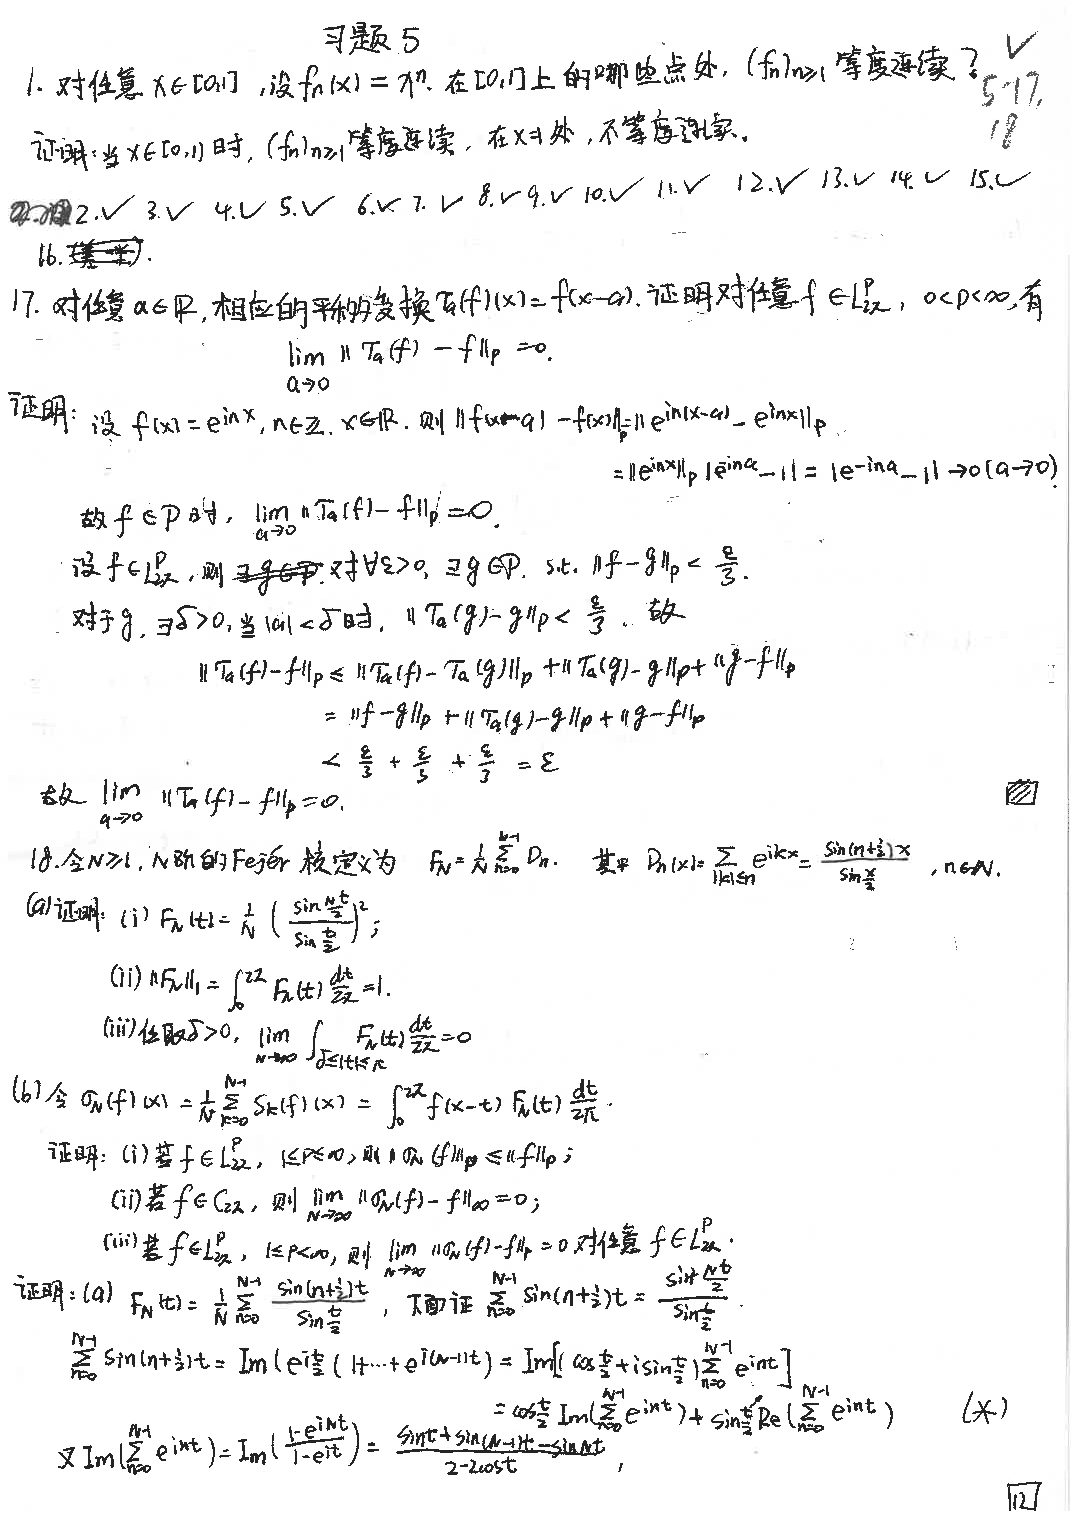
\includepdf[pages={1-1}]{5_17_18.pdf}

18. 令$N\geq 1$, $N$阶的Fejer核定义为
\[F_N=\frac{1}{N}\sum_{n=0}^{N-1}D_n,\]
其中
\[D_n(x)=\sum_{|k|\leq n}e^{ikx}=\frac{sin(n+\frac{1}{2})x}{\sin \frac{x}{2}},n\in\mathbb{N}.\]
\begin{itemize}
	\item[(a)] 证明:
	\begin{itemize}
		\item[(i)] $F_N(t)=\frac{1}{N}\left(\frac{\sin \frac{Nt}{2}}{\sin \frac{t}{2}}\right)^2$;
		\item[(ii)] $\|F_n\|_1=\int _0^{2\pi} F_N(t)\frac{dt}{2\pi}=1$;
		\item[(iii)] 任取$\delta>0$, $\lim_{N\to\infty}\int_{\delta\leq |t|\leq \pi}F_N(t)\frac{dt}{2\pi}$.
	\end{itemize}
	\item[(b)]令
	\[\sigma_N(f)(x)=\frac{1}{N}\sum_{k=0}^{N-1}S_k(f)(x)=\int_0^{2\pi}f(x-t)F_N(t)\frac{dt}{2\pi}.\]
	\begin{itemize}
		\item[(i)] 若$f\in L_{2\pi}^p$, $1\leq p\leq \infty$, 则$\|\sigma_N(f)\|_p\leq \|f\|_p$;
		\item[(ii)] 若$f\in C_{2\pi}$, 则$\lim_{N\to\infty}\|\sigma_N(f)-f\|_\infty=0$;
		\item[(iii)] 若$f\in L_{2\pi}^p$, $1\leq p<\infty$, 则$\lim_{N\to\infty}\|\sigma_{N}(f)-f\|_p=0$对任意$f\in L_{2\pi}^p$.
	\end{itemize}
\end{itemize}
\begin{proof}
	(a) (i)令$\theta=t\backslash 2$, 则
	\[
	\sum_{n=0}^{N-1}\sin(n+\frac{1}{2}t)=\sum_{n=0}^{N-1}\sin(2n+1)\theta
	=\frac{\sin^2 N\theta}{\sin \theta}.
	\]	
	故
	\[F_N(t)=\frac{1}{N}\left(\frac{\sin \frac{Nt}{2}}{\sin \frac{t}{2}}\right)^2.\]
	
	(ii) 由(i)知$F_N(t)\geq 0$, 故$\|F_N\|_1=\int_0^{2\pi} F_N(t)\frac{dt}{2\pi}$, 又对$\forall n\in\mathbb{N}$,
	\[\int_0^{2\pi}D_n(t)\frac{dt}{2\pi}=\int_0^{2\pi}1+2\cos t+\cdots+2\cos nt\frac{dt}{2\pi}=1\]
	故$\int_0^{2\pi} F_N(t)\frac{dt}{2\pi}=N\cdot \frac{1}{N}=1$.
	
	(iii) 任取$\delta>0$, 
	\[\int_{\delta\leq |t|\leq \pi}F_N(t)\frac{dt}{2\pi}=\frac{2}{N}\int_{\delta\leq t\leq \pi}\left(\frac{\sin \frac{Nt}{2}}{\sin \frac{t}{2}}\right)^2\frac{dt}{2\pi}\leq \frac{2}{N}\int_{\delta\leq t\leq \pi}\left(\frac{1}{\sin \frac{t}{2}}\right)^2\frac{dt}{2\pi}\to 0(N\to\infty).\]
	
	(b) (i) 注意到$\sigma_N(f)=f*F_N$, 则由广义Minkowski不等式(第三章习题13)知
	\[\|\sigma_N(f)\|_p=\|f*F_N\|_p\leq \|f\|_p\|F_N\|_1=\|f\|_p.\]
	
	(ii) 对$\forall \e>0$, 由于$f\in C_{2\pi}$,存在$\delta>0$, 当$|t|<\delta$时
	\[|f(x-t)-f(x)|<\frac{\e}{2},\forall x\in \mathbb{R}\]
	则
	\[\begin{split}
	\sigma_N(f)(x)-f(x)=&\int_0^{2\pi} f(x-t)F_N(t)\frac{dt}{2\pi}-\int_0^{2\pi} f(x)F_N(t)\frac{dt}{2\pi}\\
	=&\int_0^{2\pi} (f(x-t)-f(x))F_N(t)\frac{dt}{2\pi}\\
	=&\int_{-\pi}^{\pi} (f(x-t)-f(x))F_N(t)\frac{dt}{2\pi}\\
	=&\int_{-\delta}^\delta+\int_{\delta \leq |t| \leq \pi}(f(x-t)-f(x))F_N(t)\frac{dt}{2\pi}
	\end{split}\]
	其中
	\[|\int_{-\delta}^\delta(f(x-t)-f(x))F_N(t)\frac{dt}{2\pi}|<\frac{\e}{2}\int_{-\pi}^\pi F_N(t)\frac{dt}{2\pi}=\frac{\e}{2}.\]
	\[\int_{\delta \leq |t| \leq \pi}(f(x-t)-f(x))F_N(t)\frac{dt}{2\pi}\leq \|f\|_{\infty}\int_{\delta\leq|t|\leq \pi}F_N(t)\frac{dt}{2\pi}<\frac{\e}{2}\text{(当N充分大)},\]
	故$|\sigma_N(f)(x)-f(x)|<\e,\forall x\in\mathbb{R}$(当$N$充分大),所以$\lim_{N\to\infty}\|\sigma_N(f)-f\|_\infty=0$.
	
	(iii) 设$f\in L_{2\pi}^p$, $1\leq p<\infty$. 对任意$\e>0$, 存在$g\in C_{2\pi}$使得$\|g-f\|_p<\frac{\e}{3}$. 由(ii)知存在$N_1$, 当$N>N_1$时
	$\|\sigma_N(g)-g\|_p\leq \|\sigma_N(g)-g\|_\infty<\frac{\e}{3},$
	则由(i)知
	\[\begin{split}
	\|\sigma_N(f)-f\|_p\leq &\|\sigma_N(f)-\sigma_N(g)\|_p+\|\sigma_N(g)-g\|_p+\|g-f\|_p\\
	\leq& \|f-g\|_p+\frac{\e}{3}+\|f-g\|_p<\e, 
	\end{split}\]
	故$\lim_{N\to\infty}\|\sigma_{N}(f)-f\|_p=0$.
\end{proof}
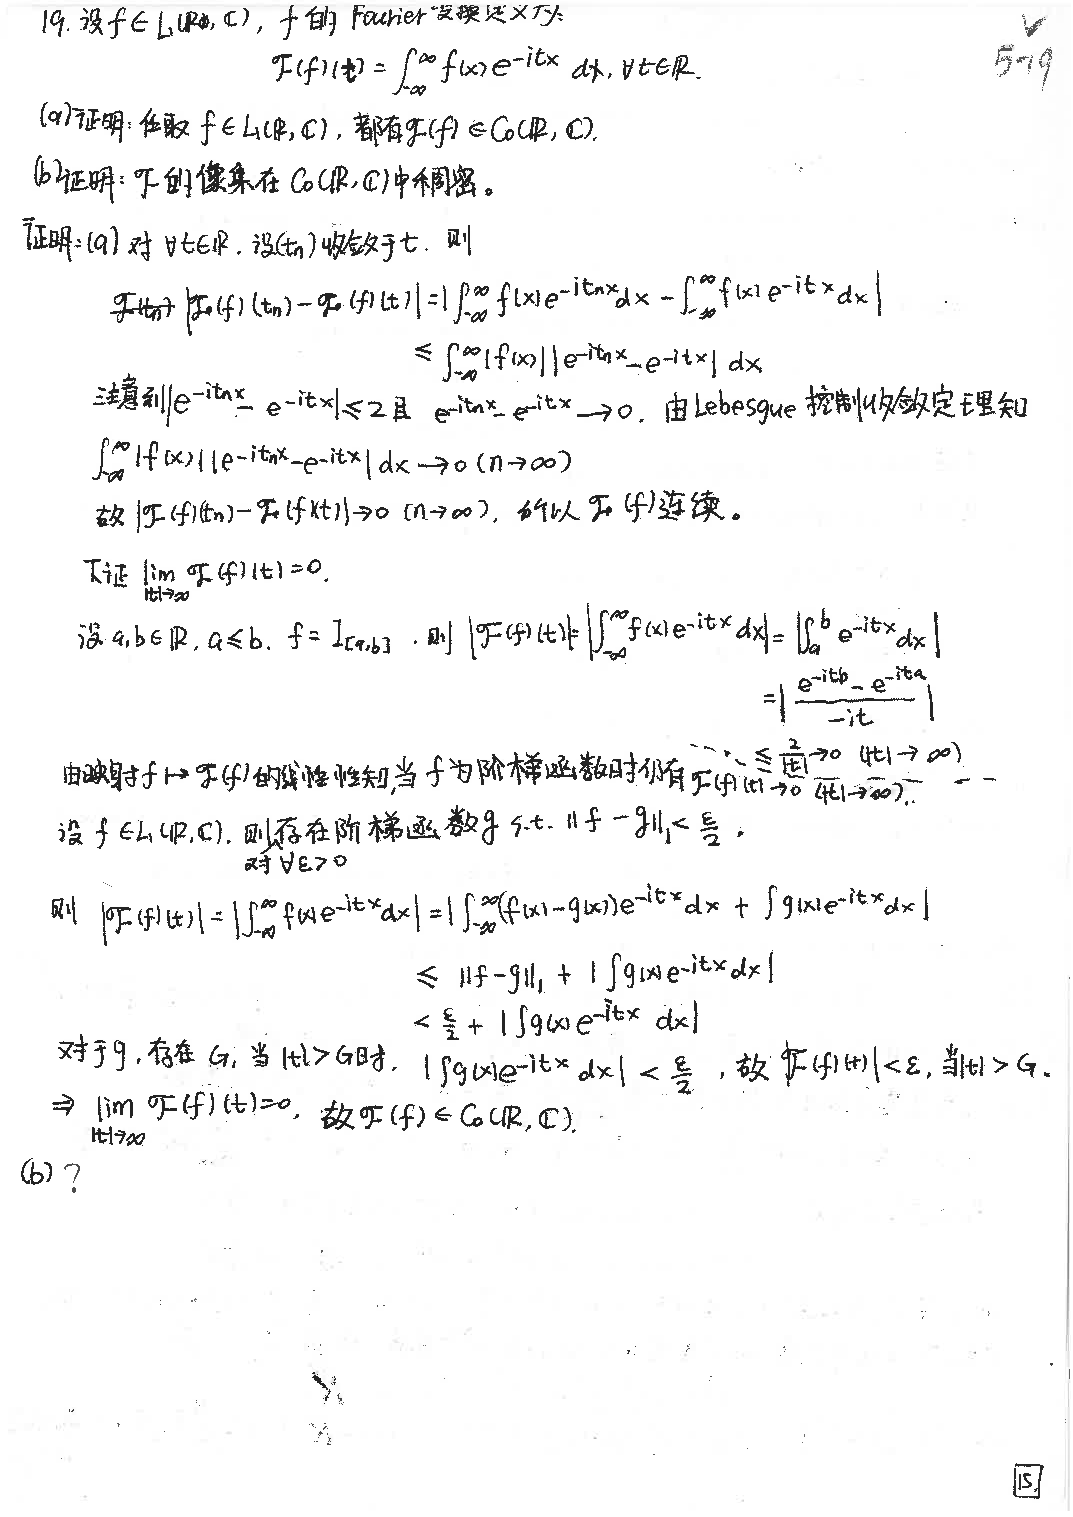
\includepdf[pages={1-1}]{5_19.pdf}

\section{第六章 习题}
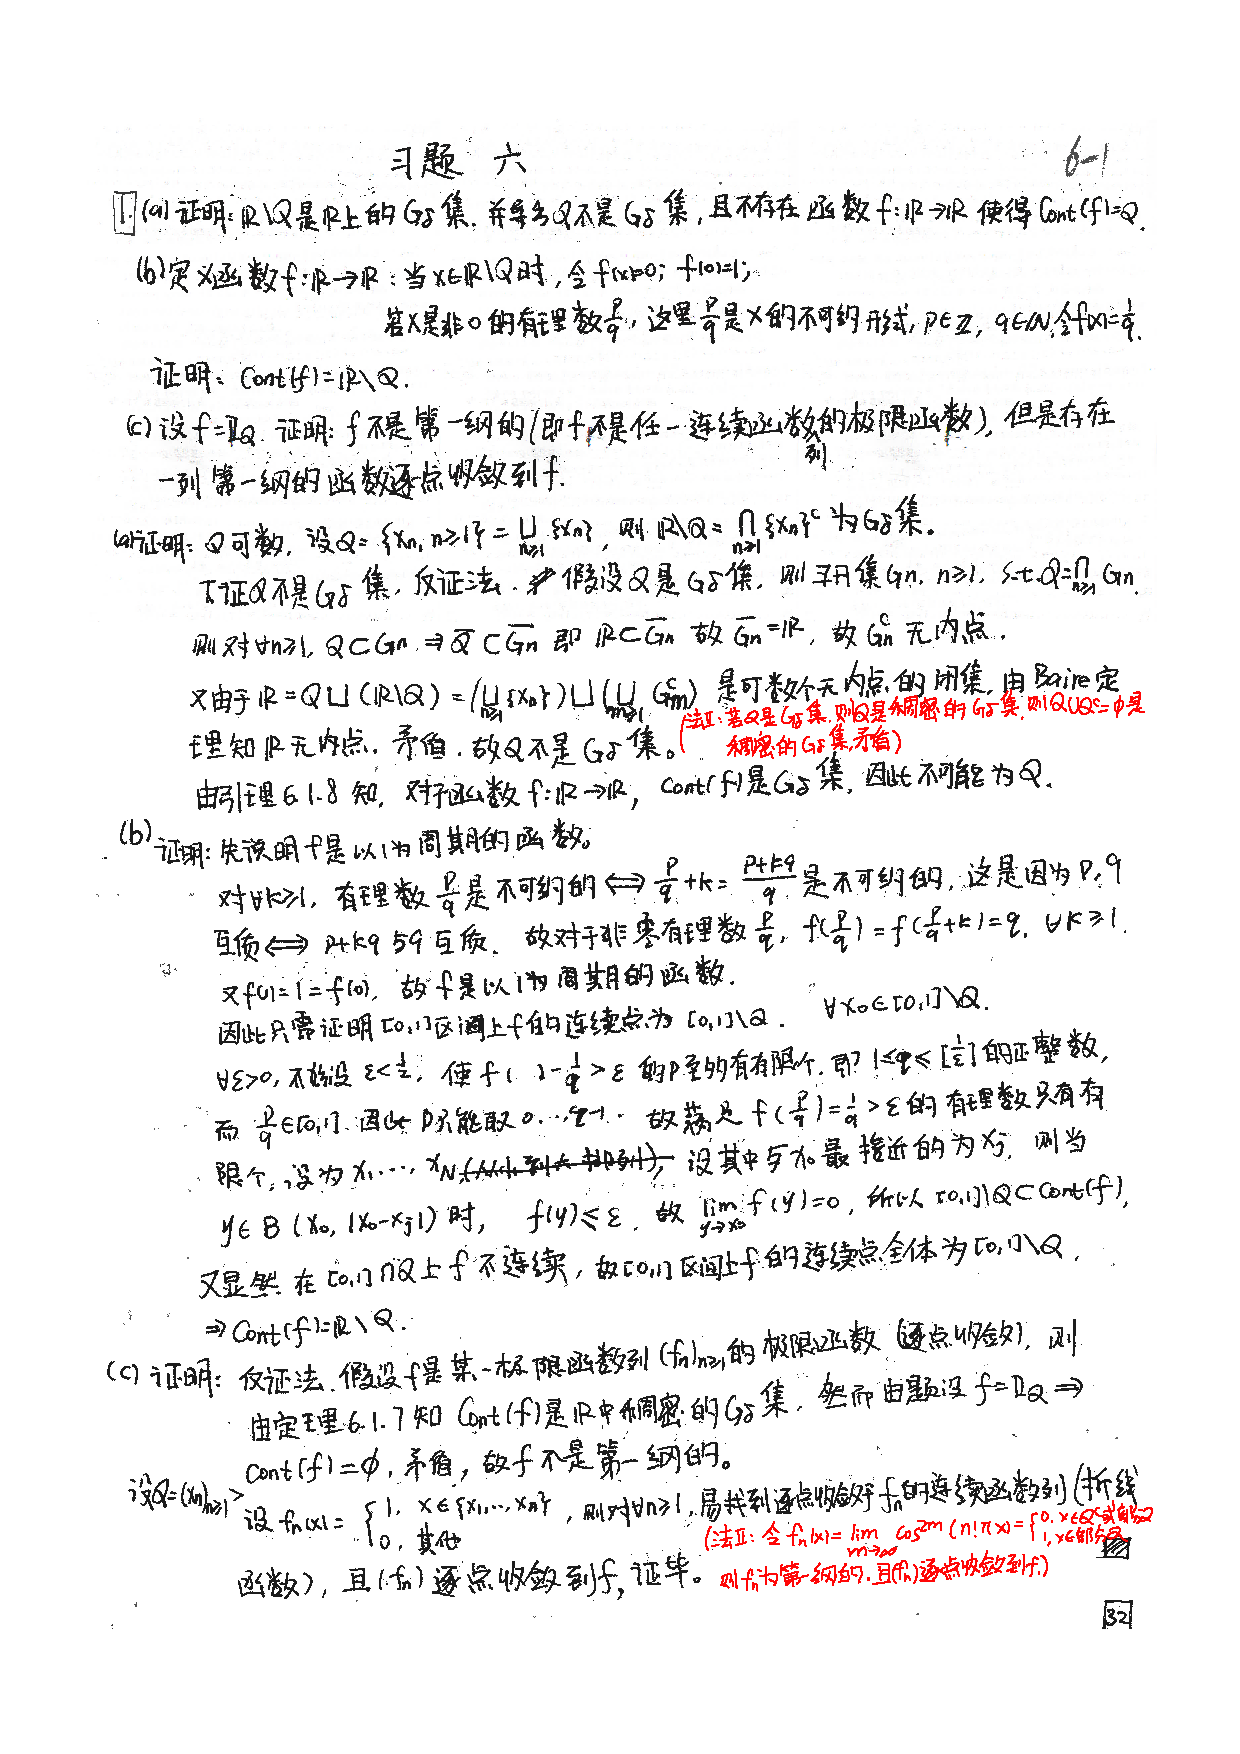
\includepdf[pages={1-1}]{6_1.pdf}
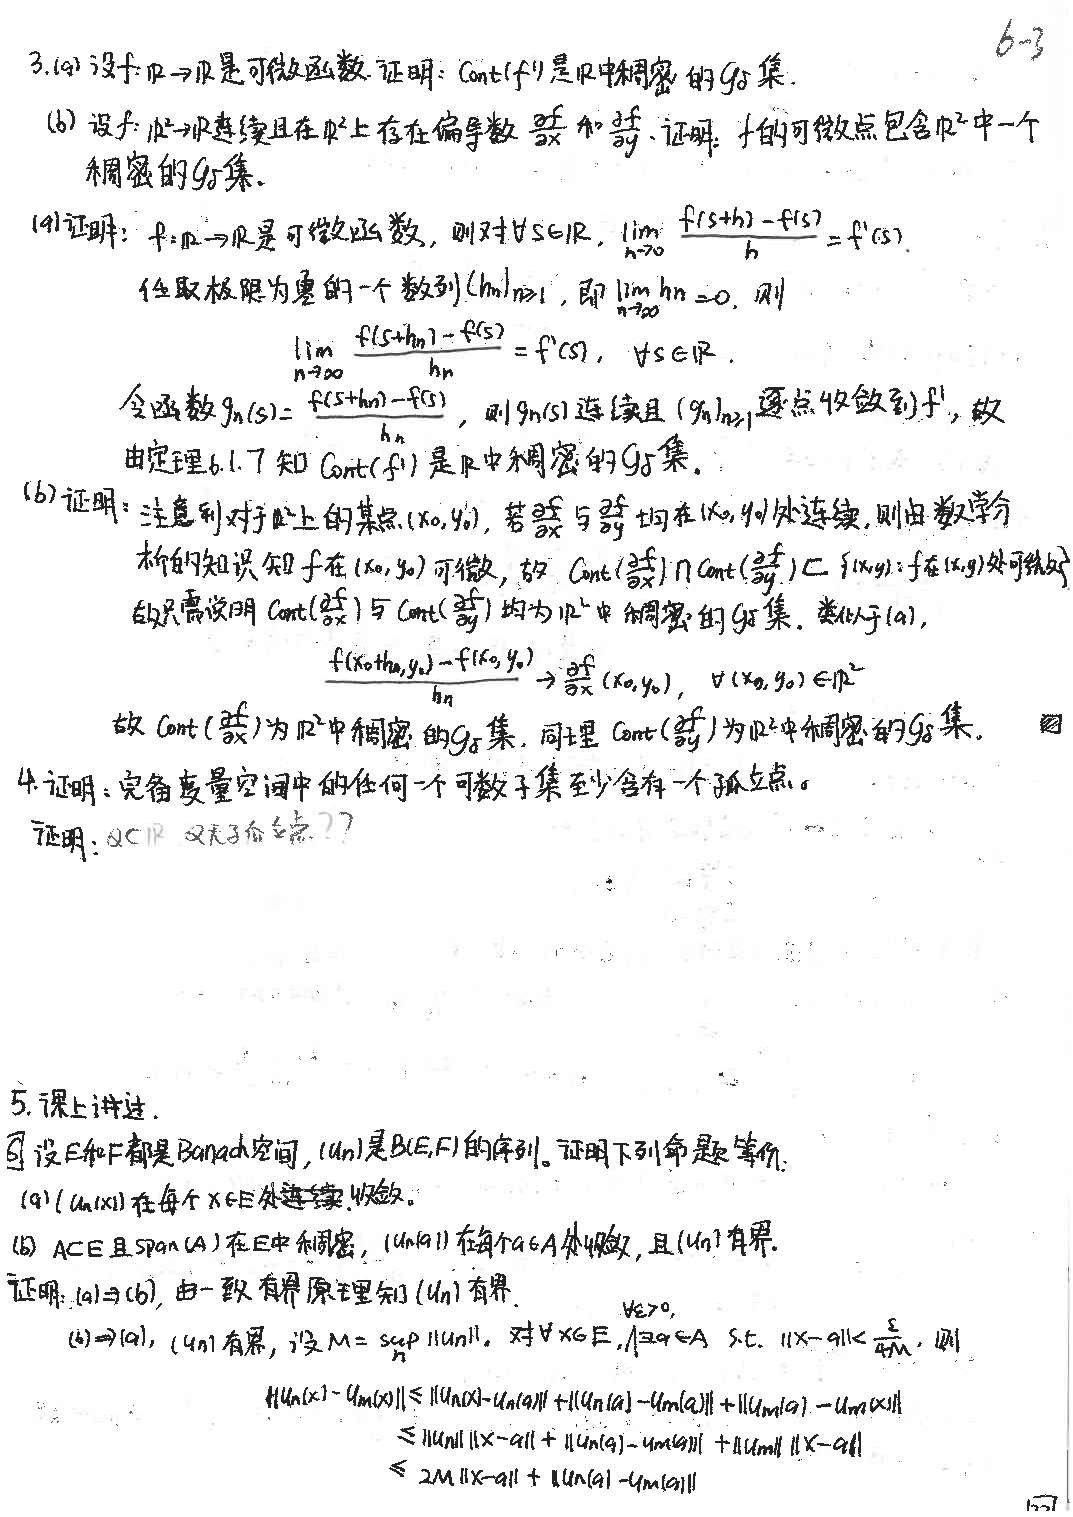
\includepdf[pages={1-1}]{6_3.pdf}
\clearpage
6. [作业]设$E$和$F$都是Banach空间,$(u_n)$是$B(E,F)$的序列。证明下列命题等价:
\begin{itemize}
	\item[(a)] $(u_n(x))$在每个$x\in E$处收敛。
	\item[(b)] $A\subset E$且$\mathrm{span}(A)$在$E$中稠密,$(u_n(a))$在每个$a$处收敛,$(u_n)$有界。
\end{itemize}
\begin{proof}
	(a)$\Rightarrow$(b):由一致有界原理可知$(u_n)$有界。
	
	(b)$\Rightarrow$(a):$(u_n)$有界,设$M=\sup_n\|u_n\|$. 对任意$x\in E$, $\forall\e>0$, 存在$a\in \mathrm{span}(A)$, s.t. $\|x-a\|<\frac{\e}{4M}$, 则
	\begin{equation*}
	\begin{split}
	\|u_n(x)-u_m(x)\|\leq& \|u_n(x)-u_n(a)\|+\|u_n(a)-u_m(a)\|+\|u_m(a)-u_m(x)\|\\
	\leq& \|u_n\|\|x-a\|+\|u_n(a)-u_m(a)\|+\|u_m\|\|x-a\|\\
	\leq& 2M\|x-a\|+\|u_n(a)-u_m(a)\|
	\end{split}
	\end{equation*}
	又由于$(u_n(a))$收敛,存在$N$, s.t. $n,m\geq N$时$\|u_n(a)-u_m(a)\|<\frac{\e}{2}$, 故
	$$\|u_n(x)-u_m(x)\|<\frac{\e}{2}+\frac{\e}{2}=\e,$$
	故$(u_n(x))$是Cauchy列,由$F$完备知$(u_n(x))$收敛。
\end{proof}
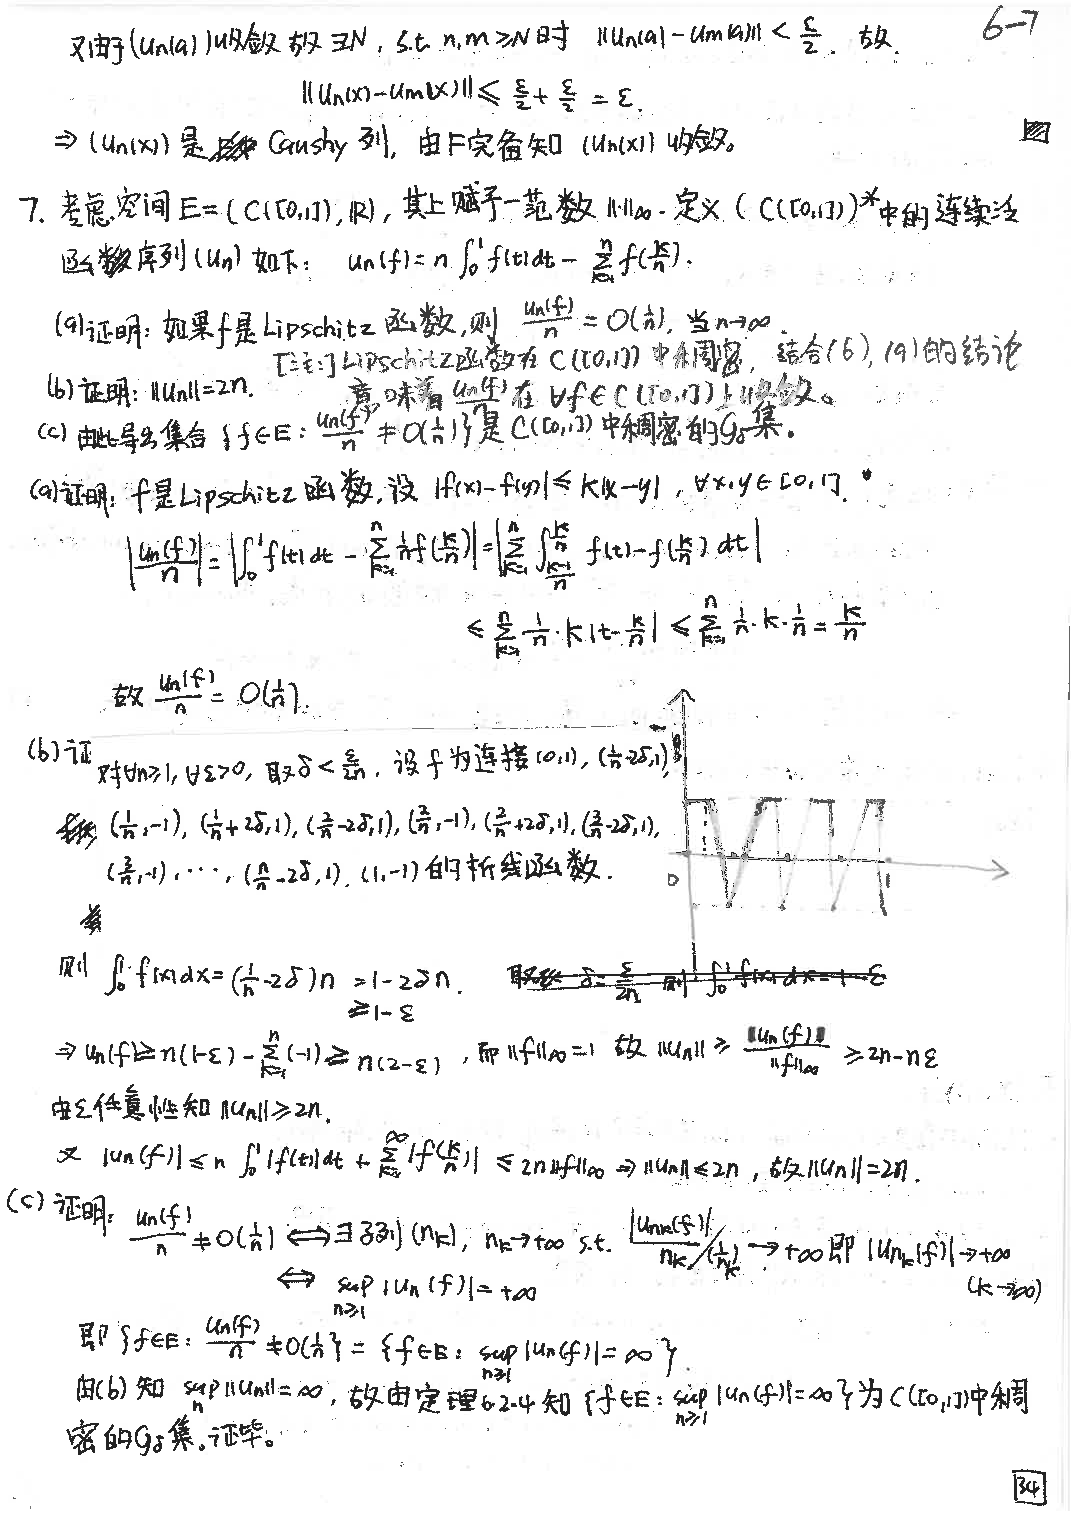
\includepdf[pages={1-1}]{6_7.pdf}
8.  [作业]设$E$是$(C([0,1]),\|\cdot\|_\infty)$的闭向量子空间,并假设$E$中的元素都是Lipschitz函数。
\begin{itemize}
	\item[(a)] 设$x,y\in[0,1]$且$x\ne y$, 定义泛函$\Phi_{x,y}:E\to\mathbb{R}$为
	\begin{equation*}
	\Phi_{x,y}(f)=\frac{f(y)-f(x)}{y-x},
	\end{equation*}
	证明:$\{\Phi_{x,y}:x,y\in[0,1],x\ne y\}$是$E^*$中的有界集。
	\item[(b)] 导出$E$中的闭单位球在$[0,1]$上等度连续,且$\dim E<\infty$.
\end{itemize}
\begin{proof}
	(a)$\Phi_{x,y}$连续: 对$\forall f\in E$, $\|\Phi_{x,y}(f)\|\leq \frac{2\|f\|}{|y-x|}$, 
	则$\Phi_{x,y}$连续且$\|\Phi_{x,y}\|\leq \frac{2}{|y-x|}$.
	
	$\forall f\in E$, 存在$K_f>0$, $|f(y)-f(x)|\leq K_f|y-x|$, $\forall x,y\in[0,1]$, 则
	$$|\Phi_{x,y}(f)|\leq K_f<\infty,\forall x,y\in[0,1],x\ne y,$$
	则$\sup_{x\ne y}|\Phi_{x,y}(f)|\leq K_f$, 由一致有界原理知$\{\Phi_{x,y}:x,y\in[0,1],x\ne y\}$有界。
	
	(b)由(a)知$\{\Phi_{x,y}:x,y\in[0,1],x\ne y\}$是$E^*$中的有界集,设$M=\sup_{x\ne y}\|\Phi_{x,y}\|$. $\forall f\in \overline{B_E}$, 即$\|f\|\leq 1$, 则$|\Phi_{x,y}(f)|\leq \|\Phi_{x,y}\|\|f\|\leq M\|f\|\leq M$, 则
	$$|f(y)-f(x)|\leq M|x-y|,\forall f\in\overline{B_E},$$
	故$\overline{B_E}$中的元素等度连续,又对$\forall x\in[0,1]$, $\|f(x)\|\leq\|f\|\leq 1$, 则轨道$\{f(x),f\in\overline{B_E}\}$相对紧,则由Ascoli定理$\overline{B_E}$在$C([0,1])$中紧,故$\dim E<\infty$. 
\end{proof}

10. [习题课]设$E,F$都是Banach空间,$u\in\mathcal{B}(E,F)$并满足$u(B_E)$在$B_F$中稠密。
\begin{enumerate}
	\item[(a)] 计算$\|u\|$.
	\item[(b)] 证明:$u(B_E)=B_F$. 因此$u$是满射。
	\item[(c)] 设$v$为$E/\ker u$到$F$的映射并满足$v\circ q=u$, 这里$q:E\to E/\ker u$是商映射。证明:$v$是从$E/\ker u$到$F$上的等距映射。
\end{enumerate}
\begin{proof}
	(a) 由题意知$u(B_E)\subset B_F$, 则$u(\overline{B_E})\subset \overline{u(B_E)}\subset \overline{B_F}$, 则$\|u\|\leq 1$. 又由于$B_F\subset \overline{u(B_E)}$, 对任意$\e>0$, 取$y\in B_F$满足$\|y\|=1-\frac{\e}{2}$, 则存在$x\in B_E$, $\|u(x)-y\|<\frac{\e}{2}$,
	则
	\begin{equation*}
	\|u\|\geq \|u(x)\|\geq \|y\|-\|u(x)-y\|\geq 1-\e,
	\end{equation*} 
	故$\|u\|=1$.
	
	(b) 由题设,$B_F\subset \overline{u(B_E)}$, 下证$B_F\subset u(B_E)$. 
	
	设$y\in B_F$, 对任意$0<q<1$, 存在$x_0\in B_E$, s.t. $$\|y-u(x_0)\|<q,$$ 
	取$y_1=\frac{1}{q}[y-u(x_0)]$, 则$\|y_1\|<1$, 即$y_1\in B_F$, 则存在$x_1\in  B_E$, $$\|y_1-u(x_1)\|<q,$$
	取$y_2=\frac{1}{q}[y_1-u(x_1)]$. 如此进行下去,可得一列$(y_n)\subset B_F$及相应的$(x_n)\subset B_E$, s.t.
	$$\|y_n-u(x_n)\|<q,n\geq 1.$$
	由以上构造过程可知
	\begin{equation*}
	\begin{split}
	y=u(x_0)+qy_1=&u(x_0)+q[u(x_1)+qy_2]\\
	=&u(x_0)+qu(x_1)+\cdots+q^nu(x_n)+q^{n+1}y_{n+1}\\
	=&u(\sum_{k=0}^n q^kx_k)+q^{n+1}y_{n+1},
	\end{split}
	\end{equation*}
	注意到级数$\sum_{k\geq0} q^kx_k$绝对收敛且$E$完备,可知该级数收敛于某点$x\in E$, 且
	$$\|x\|\leq \sum_{n\geq 0}q^n\|x_n\|<\frac{1}{1-q},$$
	即$x\in \frac{1}{1-q}B_E$. 又由$u$连续, 则$y=u(x)$, 故$$y\in \frac{1}{1-q}u(B_E)\Rightarrow (1-q)y\in u(B_E)\Rightarrow (1-q)B_F\subset u(B_E),$$ 
	则$B_F=\cup_{0<q<1}(1-q)B_F\subset u(B_E)$, 故$B_F\subset u(B_E)$, 所以$B_F=u(B_E)$.
	
	
	(c) 设$A=\ker u$.
	
	$v$连续:对$\forall e\in E$, 有
	\[\|v(e+A)=\|u(e)\|=u(e+y)\leq \|u\|\|e+y\|,\forall y\in A,\]
	对$y$取下确界则$\|v(e+A)\|\leq \|u\|\|e+A\|$, 故$v$连续且$\|v\|\leq\|u\|$.
	
	$v$是满射:对任意$f\in F$, 存在$e\in E$, s.t.$u(e)=v(e+A)=f$, 所以$v$是满射。
	
	$v$是单射:若$e\in E$满足$v(e+A)=u(e)=0$,则$e\in A$, 故$e+A=0+A$, 所以$v$是单射。因此$v$是连续的线性双射,由开映射定理$v^{-1}$是连续的。
	
	下面想说明$E/A$与$F$等距同构,先证明$q(B_E)=B_{E\backslash A}$.  首先,$\|e\|<1$时$\|e+A\|<1$, 故$q(B_E)\subset B_{E\backslash A}$. 另一方面,$\|e+A\|<1$时,存在$a\in A$使得$\|e+a\|<1$, 且$q(e+a)=e+A$, 因此$B_{E\backslash A}\subset q(B_E)$, 故$B_{E\backslash A}=q(B_E)$. 则
	\begin{equation}\label{6.10}
	B_F=u(B_E)=v\circ q(B_E)=v(B_{E\backslash A}),
	\end{equation}
	故
	$$v(\overline{B_{E\backslash A}})\subset \overline{v(B_{E\backslash A})}\subset \overline{B_F}\RA \|v\|\leq 1,$$
	且由式(\ref{6.10})得$v^{-1}(B_F)=B_{E\backslash A}$, 同理可证$\|v^{-1}\|\leq 1$, 因此
	$$\|e+A\|= \|v(e+A)\|,\forall e\in E.$$
\end{proof}

13. [习题课](a) 设$E$是赋范空间,$F$是$E$的向量子空间。证明:若$F\ne E$, 则$F$在$E$中的内部是空集。

(b) 由此证明所有的多项式构成的空间不能赋予完备范数。
\begin{proof}
	(a) 反证法,若$\mathring{F}\ne \varnothing$, 则存在$B(x_0,r)\subset F$, 这等价于$B(0,r)\subset F$且$x_0\in F$. 由于$F\ne E$, 存在$x\in E$, $x\notin F$, 而$\frac{r}{2\|x\|}x\in B(0,r)\subset F$, 故$x\in F$, 矛盾。
	
	(b) 反证法。所有多项式构成的空间记为$\mathcal{P}$, 注意到
	$$\mathcal{P}=\cup_{n=1}^\infty \mathrm{span}\{ 1,x,\cdots,x^n\}=\cup_{n=1}^\infty \mathcal{P}_n,$$
	这里$\mathcal{P}_n=\mathrm{span}\{ 1,x,\cdots,x^n\}$, $\mathcal{P}_n$有限维所以是闭的。设在某个范数$\|\cdot\|$下, $(\mathcal{P},\|\cdot\|)$是完备的, 则由定理6.1.4, $\cup_{n=1}^\infty \mathring{\mathcal{P}_n}$在$\mathcal{P}$中稠密,然而由(a)知对任意$n\geq 1$, $\mathring{\mathcal{P}_n}=\varnothing$, 则$\varnothing$在$\mathcal{P}$中稠密,矛盾。
\end{proof}

14. [习题课]设$E$是Banach空间,$F$和$G$都是$E$的闭向量子空间,并且$F+G$也是闭向量子空间。证明:存在一个常数$C\geq 0$, 使得$\forall x\in F+G$, 存在$(f,g)\in E\times G$, 满足
$$x=f+g,\|f\|\leq C\|x\|,\|g\|\leq C\|x\|.$$
\begin{proof}
	设$u:F\times G\to F+G$, $(f,g)\mapsto f+g$, 显然$u$是满射,又
	\begin{equation*}
	\|f+g\|\leq 2\max\{\|f\|,\|g\|\}=2\|(f,g)\|,
	\end{equation*}
	故$u$连续,由开映射定理,存在$c_0>0$, s.t. $c_0B_{F+G}\subset u(B_{F\times G})$, 则
	\begin{equation*}
	\frac{c_0}{2}\overline{B_{F+G}}\subset c_0B_{F+G}\subset u(B_{F\times G}),
	\end{equation*}
	令$C=\frac{2}{c_0}$, 则$\frac{1}{C}\overline{B_{F+G}}\subset u(B_{F\times G})$, 对任意$x\in F+G$, $\frac{1}{C\|x\|}x\in \frac{1}{C}\overline{B_{F+G}}$, 故存在$(f_1,g_1)\in E\times F$, 使得
	\begin{equation*}
	\frac{x}{C\|x\|}=f_1+g_1\mbox{ 且 }\max\{\|f_1\|,\|g_1\|\}<1,
	\end{equation*} 
	则$x=C\|x\|f_1+C\|x\|g_1$, 令$f=C\|x\|f_1, g=C\|x\|g_1$即可。
\end{proof}

15. [习题课]设$H$是Hilbert空间,且线性映射$u:H\to H$满足
\begin{equation*}
\la u(x),y\ra=\la x,u(y)\ra,\forall x,y\in H,
\end{equation*}
证明:$u$连续。
\begin{proof}
	设$(x_n)\subset H$, $x_n\to 0$, $u(x_n)\to y$, 由闭图像定理,只需证明$y=0$.
	对任意$z\in H$, 
	\begin{equation*}
	\la u(x_n),z\ra=\la x_n,u(z)\ra\to 0(n\to\infty),
	\end{equation*}
	又$\lim_{n\to\infty}\la u(x_n),z\ra=\la y,z\ra$, 则$\la y,z\ra=0$, $\forall z\in H$,
	故$y=0$.
\end{proof}

16. [作业题]设$X=C^1([0,1],\mathbb{R})$, 即由$[0,1]$上连续可导的函数构成的集合,其上赋予连续一致范数$\|\cdot\|_\infty$, 并设$Y=C([0,1],\mathbb{R})$, 其上也赋予一致范数。考虑映射$u:X\to Y$, $u(f)=f'$.

证明:$u$的图像是闭的,但$u$不连续。解释该结论的意义。
\begin{proof}
	设$x_n,x,y\in X$, $x_n\to 0$, $u(x_n)=x_n'\to y$, 则对任意$t\in[0,1]$, 
	$$\int_0^t x_n'dt\to\int_0^t y(t)dt,$$
	即$x_n(t)-x_n(0)\to\int_0^t y(t)dt$, 又$x_n(t)-x_n(0)\to 0-0$, 故$0=\int_0^t y(t)dt$, 求导知$y=0$, 所以$u$的图像是闭的。
	
	$u$不连续:取$x_n(t)=t^n$, 则$\|x_n\|=1$, 但是$\|u(x_n)\|=\|x_n'\|=n\|t^{n-1}\|=n\to+\infty(n\to\infty)$, 故$u$不连续。
	
	意义:当$X$不完备时,闭图像定理不成立。
\end{proof}

19. [作业题]设$(X,\mathcal{A},\mu)$是$\sigma$-有限的测度空间。
\begin{itemize}
	\item[(a)] 假设当$1\leq p<q\leq\infty$时,有$L_q(X,\mathcal{A},\mu)\subset L_p(X,\mathcal{A},\mu)$. 证明:存在常数$C\geq 0$, 使得对 任意$f\in L_q(X,\mathcal{A},\mu)$, 有$\|f\|_p\leq C\|f\|_q$.
	\item[(b)] 导出以下命题的等价性:
	\begin{itemize}
		\item[(i)] 存在$1\leq p<q\leq \infty$, 使得$L_q(X,\mathcal{A},\mu)\subset L_p(X,\mathcal{A},\mu)$.
		\item[(ii)] $\mu(X)<\infty$.
		\item[(iii)] 任取$1\leq p<q\leq \infty$, 有$L_q(X,\mathcal{A},\mu)\subset L_p(X,\mathcal{A},\mu)$. 
	\end{itemize}
\end{itemize}
\begin{proof}
	(a) $X$是$\sigma$-有限的,即存在一列递增的可测集$(A_n)_{n\geq 1}$, s.t. $X=\cup_{n\geq 1}A_n$且$\mu(A_n)<\infty$, $\forall n\geq 1$. 考虑线性映射$I_n:L_q\to L_p$, $f\mapsto fI_{A_n}$, 则由第三章习题11知
	$$\|I_n(f)\|_p=(\int_{A_n}|f|^pd\mu)^{\frac{1}{p}}\leq \mu(A_n)^{\frac{1}{p}-\frac{1}{q}}(\int_{A_n}|f|^qd\mu)^{\frac{1}{q}}=\mu(A_n)^{\frac{1}{p}-\frac{1}{q}}\|f\|_q,$$
	故$\|I_n\|\leq \mu(A_n)^{\frac{1}{p}-\frac{1}{q}}$, 则 $I_n$连续。设映射$I:L_q\to L_p$, $f\mapsto f$, 则$(I_n)_{n\geq 1}$逐点收敛到$I$, 由推论$6.2.5$知$I$连续且$\sup_{n}\|I_n\|<\infty$且
	$\|I\|\leq \liminf_{n\to\infty} \|I_n\|$, 设$C=\liminf_{n\to\infty} \|I_n\|$, 则$\|f\|_p\leq C\|f\|_q$.
	
	(b) (ii)$\RA$(iii): 参见第三章习题11; (iii)$\RA$(i): 显然;
	
	(i)$\RA$(ii): 反证法,假设$\mu(X)=\infty$, 则对任意$n\in\mathbb N$, 存在可测集$B_n$, $\mu(B_n)>n$. 取$f=I_{B_n}$, 则$\|f\|_p=\mu(B_n)^{\frac{1}{p}}$, $\|f\|_q=\mu(B_n)^{\frac{1}{q}}$, 则$$\mu(B_n)^{\frac{1}{p}}\leq C\mu(B_n)^{\frac{1}{q}} \RA\mu(B_n)^{\frac{1}{p}-\frac{1}{q}}\leq C\RA n^{\frac{1}{p}-\frac{1}{q}}\leq C\RA C=\infty,$$
	矛盾。
\end{proof}

%
%18. 设$E$是可分Banach空间且$E\ne\{0\}$, $(x_n)_{n\geq 1}$是单位球$B_E$中的稠密序列。
%\begin{enumerate}
%	\item[(a)] 证明:存在$u\in B(\ell,E)$, 使得
%	$$u((a_n)_{n\geq 1})=\sum_{n\geq 1}a_nx_n.$$
%	\item[(b)] 证明:$u$作用在$\ell_1$上的开单位球上的像集为$B_E$. 试问:$u$作用在$\ell_1$闭单位球上的像集是什么?
%	
%\end{enumerate}
20.[{\color{red}存在问题,因为借助了等价范数定理}] 设$E$是Banach空间。称$p$是$E$上的半范数,若$p$满足除了正定性以外其他所有的范数公理(即由$p(x)=0$不一定能得到$x=0$). 假设$p$还是$\sigma$-次可加的:
\begin{equation*}
\sum_{n=1}^\infty x_n\mbox{ 在 }E\mbox{ 中收敛 }\Rightarrow p(\sum_{n=1}^\infty x_n)\leq\sum_{n=1}^\infty p(x_n)\leq \infty
\end{equation*}
证明:存在常数$M\geq 0$, s.t.$p(x)\leq M(x),\forall x\in E$.

从上面这个结论导出Banach-Steinhaus定理、开映射定理和闭图像定理。
\begin{itemize}
	\item[(a)] Banach-Steinhaus定理:令$p(x)=\sup_{i\in I}\|u_i(x)\|$.
	\item[(b)] 开映射定理:设$u:E\to F$是连续线性映射,取$p(y)=\inf\{\|x\|:u(x)=y\},y\in F$.
	\item[(c)] 闭图像定理:令$p(x)=\|u(x)\|$.
\end{itemize}
\begin{proof}
	利用等价范数定理。定义$\|\cdot\|_1:E\to\mathbb{R}_+$为$\|x\|_1=\|x\|+p(x)$, $\forall x\in E$. 验证$\|\cdot\|_1$是$E$上的范数:$\|x\|_1\geq 0$, $\|x\|_1=0\Rightarrow x=0$; 正齐性显然;三角形不等式显然。
	
	验证$\|\cdot\|_1$是完备的:设级数$\sum_{n\geq 1}x_n$绝对收敛,即$\sum_{n\geq 1}\|x_n\|_1<\infty$, 则
	$$\sum_{n\geq 1}\|x_n\|<\infty\mbox{ 且 }\sum_{n\geq 1}p(x_n)<\infty,$$
	则存在$x\in E$, s.t.$\|\sum_{k=1}^n x_k-x\|\to 0$, 且存在$N$, 当$n>m>N$时,$\|\sum_{k=m}^n x_k\|<\frac{\e}{2}$, 令$n\to\infty$则$\|\sum_{k=m}^\infty x_k\|\leq\frac{\e}{2}$. 而且$p(\sum_{k=m}^\infty x_k)\leq\sum_{k=m}^\infty p(x_k)\leq \frac{\e}{2}$, 故
	\begin{equation*}
	\|\sum_{k=m}^\infty x_k\|_1=\|\sum_{k=m}^\infty x_k\|+p(\sum_{k=m}^\infty x_k)\leq \e, m>N,
	\end{equation*}
	因此$\|x-\sum_{k=1}^{m-1}x_k\|_1\leq \e,m>N$, 所以$\|\cdot\|_1$完备且$\|\cdot\|\leq\|\cdot\|_1$, 由等价范数定理,存在$M\geq 0$, 使得$\|\cdot\|_1\leq M\|\cdot\|\Rightarrow p(x)\leq M\|x\|,\forall x\in E$.
	
	(a) 若$\forall x\in E$, $\sup_{i\in I}\|u_i(x)\|<\infty$, 定义$p(x)=\sup_{i\in I}\|u_i(x)\|$, 则$p(x)$是半范数且易验证$p$满足$\sigma$-次可加性,所以$p(x)\leq M\|x\|,\forall x\in E$, 则
	$$\sup_{i\in I}\|u_i(x)\|\leq M\|x\|, \forall x\in E,$$
	则
	$$\|u_i(x)\|\leq M\|x\|,\forall x\in E\Rightarrow \|u_i\|\leq M, \forall i\Rightarrow \sup_{i}\|u_i\|\leq M,$$
	
	(b)此处设$u$为满射,想证明存在$r>0$, s.t. $rB_F\subset u(B_E)$. 令
	$$p(y)=\inf\{\|x\|:u(x)=y\},y\in F,$$
	对于任意$\alpha\in\mathbb{K}$, 
	$$p(\alpha y)=\inf \{\|x\|:u(x)=\alpha y\}=\inf\{\alpha\frac{\|x\|}{\|\alpha\|}:u(\frac{x}{\alpha})=y\}=\inf\{|\alpha|\|z\|:u(z)=y\}=|\alpha|p(y),$$
	故正齐次性满足。对任意$y_1,y_2\in E$, 设$A_1=\{x_1:u(x_1)=y_1\}$, $A_2=\{x_2:u(x_2)=y_2\}$, $A_3=\{x_3:u(x_3)=y_1+y_2\}$. 若$u(x_1)=y_1,u(x_2)=y_2$, 则
	$$u(x_1+x_2)=y_1+y_2\Rightarrow x_1+x_2\in A_3\Rightarrow p(y_1+y_2)\leq \|y_1+y_2\|\leq \|x_1\|+\|x_2\|,$$
	所以$p(x_1+y_2)\leq p(y_1)+p(y_2)$, 故$p$是半范数。
	
	验证$p$是$\sigma$-次可加的:设$\sum_{k=1}^\infty y_k$收敛,令$J_k=\{x_k:u(x_k)=y_k\}$, 若$u(x_k)=y_k$, 若$\sum_{k=1}^\infty x_k$收敛,则由$u$的连续性有$u(\sum_{k=1}^\infty x_k)=\sum_{k=1}^\infty y_k$, 故
	\begin{equation}\label{6.20}
	p(\sum_{k=1}^\infty y_k)\leq \|\sum_{k=1}^\infty x_k\|\leq\sum_{k=1}^\infty \|x_k\|,	
	\end{equation}
	若$\sum_{k=1}^\infty x_k$发散,则$\sum_{k=1}^\infty \|x_k\|=\infty$, 则(\ref{6.20})式仍然成立,因此
	$$p(\sum_{k=1}^\infty y_k)\leq\sum_{k=1}^\infty p(y_k),$$
	即$p$是$\sigma$-次可加的,故$p(y)\leq M\|y\|,\forall y\in F$, 即
	$$\inf\{\|x\|:u(x)=y\}\leq M\|y\|,$$
	因此当$\|y\|<1$时,
	$$\inf\{\|x\|:u(x)=y\}<M\Rightarrow \exists x\in E,s.t.u(x)=y\mbox{ 且 }\|x\|\leq M,$$
	故$B_F\subset u(MB_E)\Rightarrow\frac{1}{M}B_F\subset u(B_E)$. 
	
	(c)还没敲,参看笔记。
\end{proof}
\section{第七章 习题}
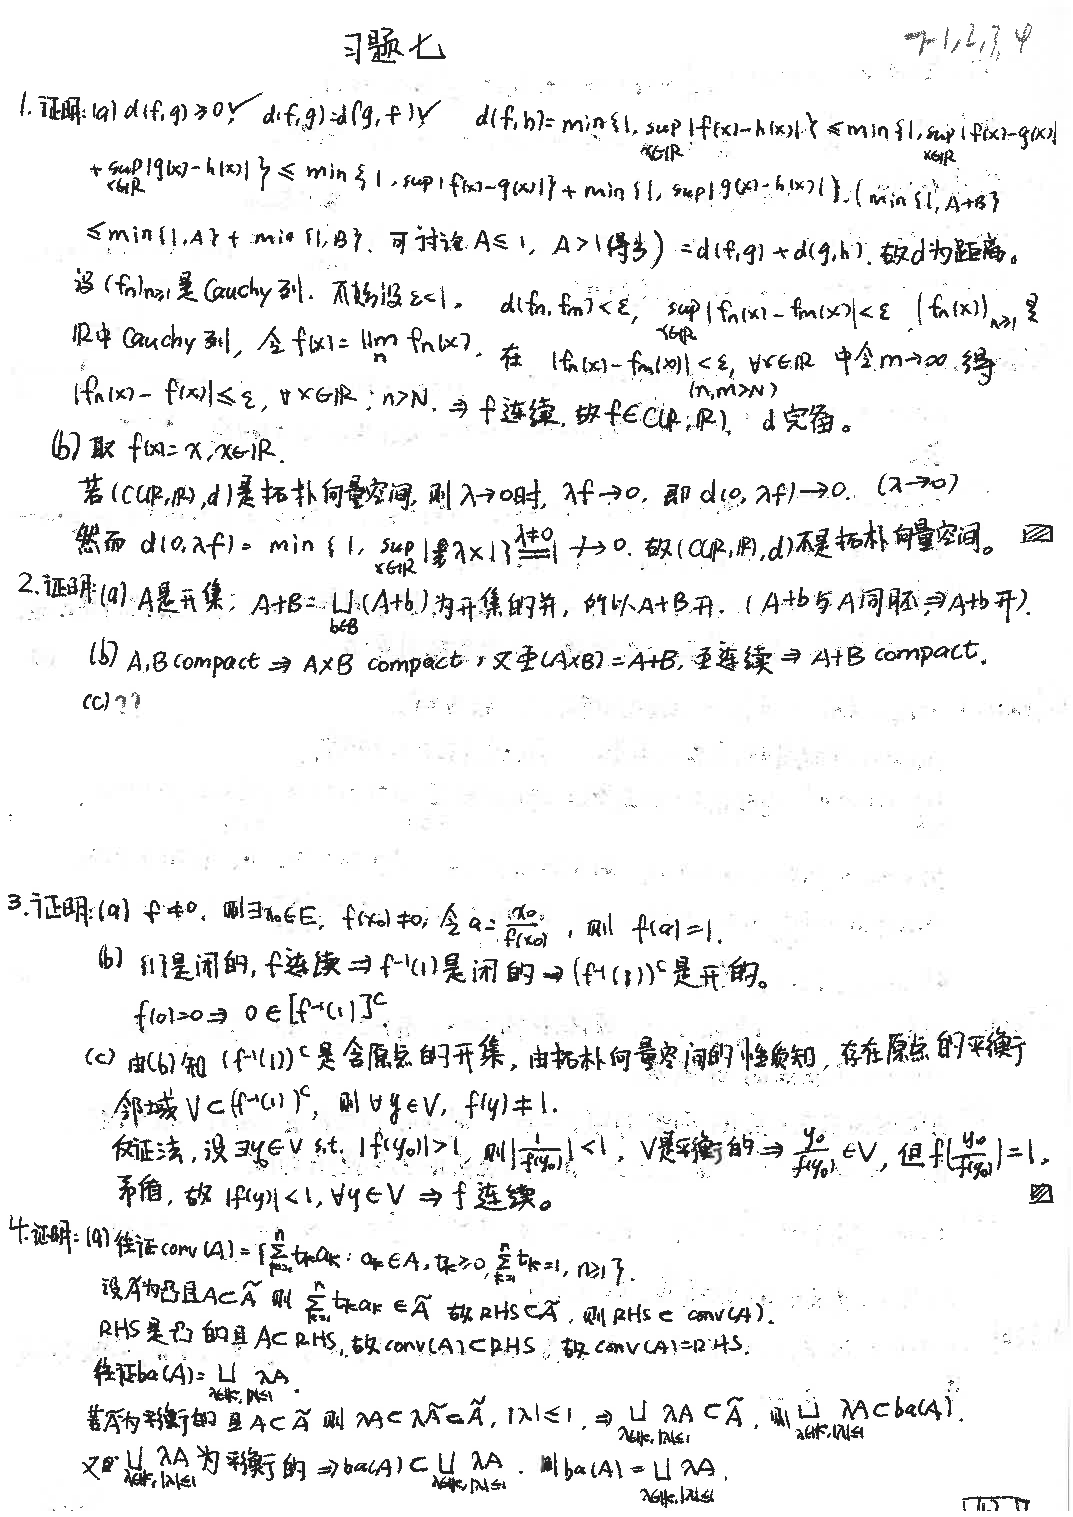
\includepdf[pages={1-1}]{7_1234.pdf}
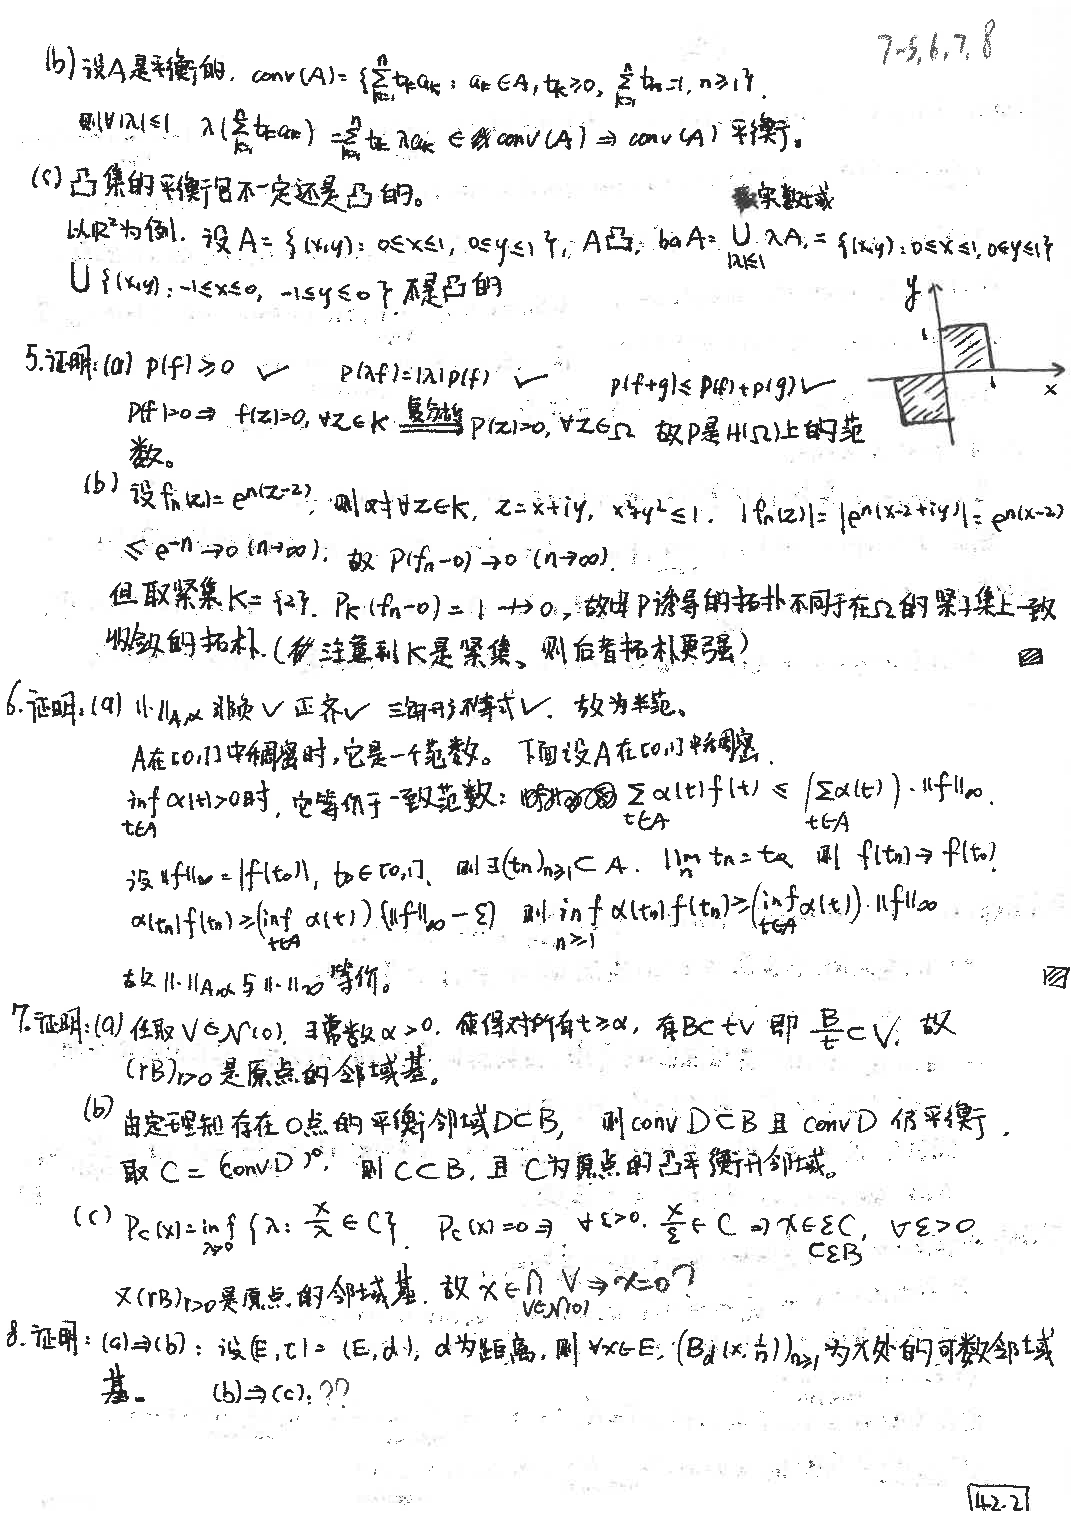
\includepdf[pages={1-1}]{7_5678.pdf}
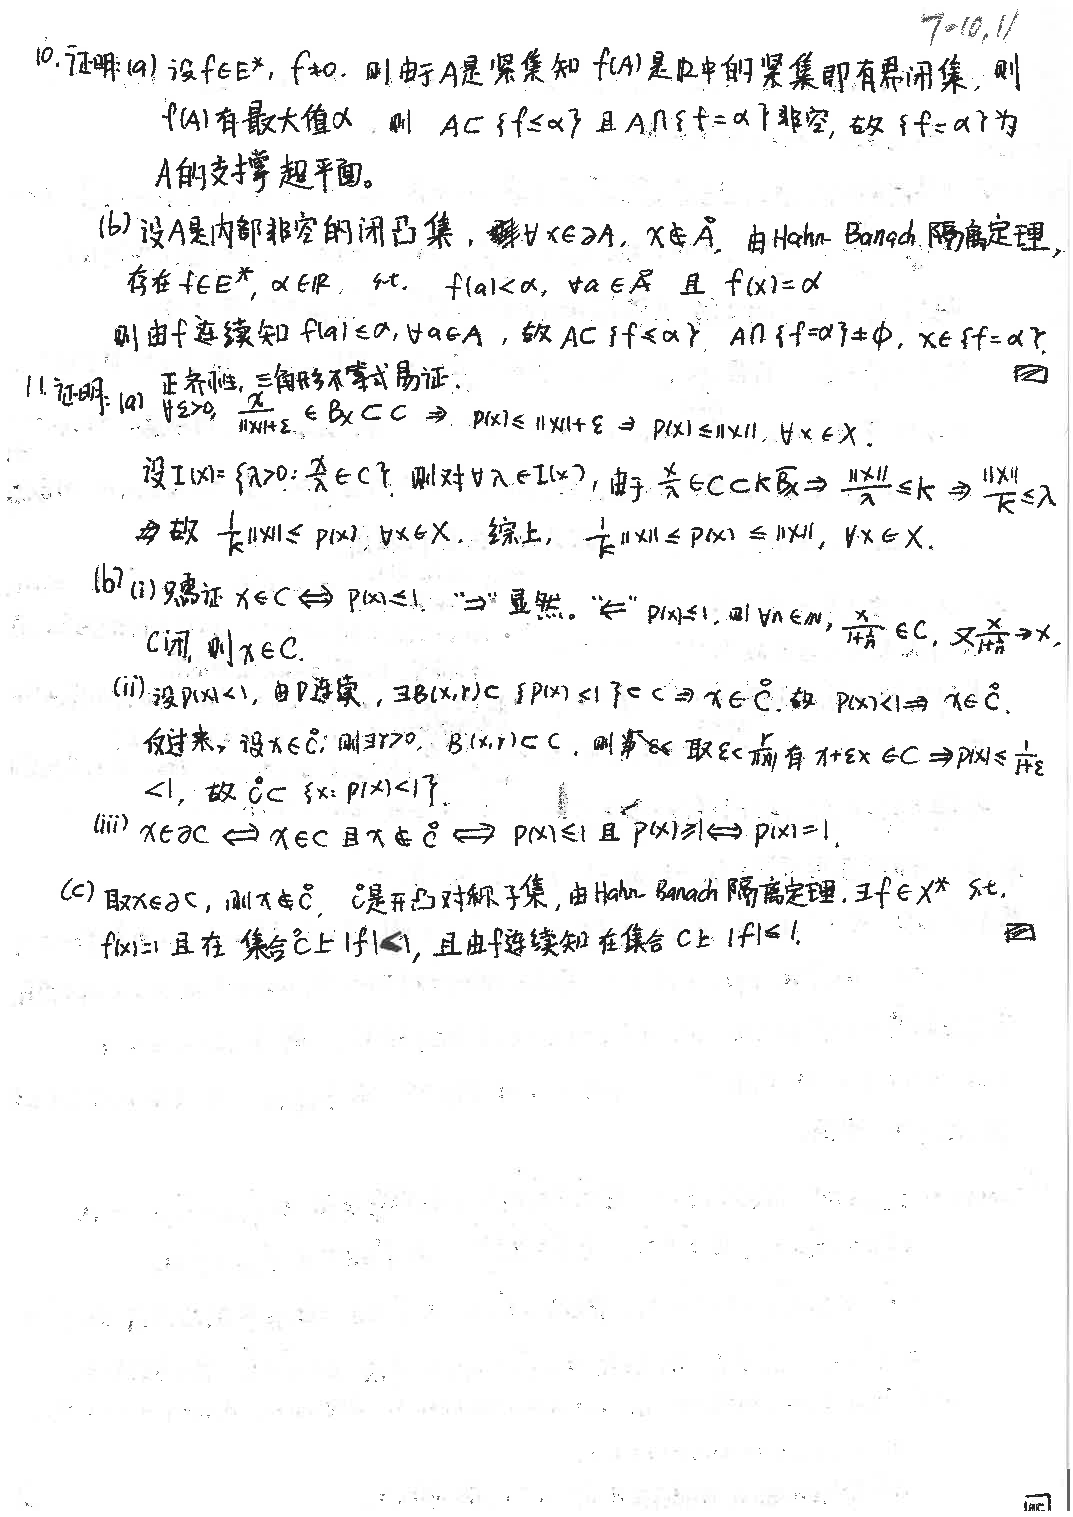
\includepdf[pages={1-1}]{7_10_11.pdf}
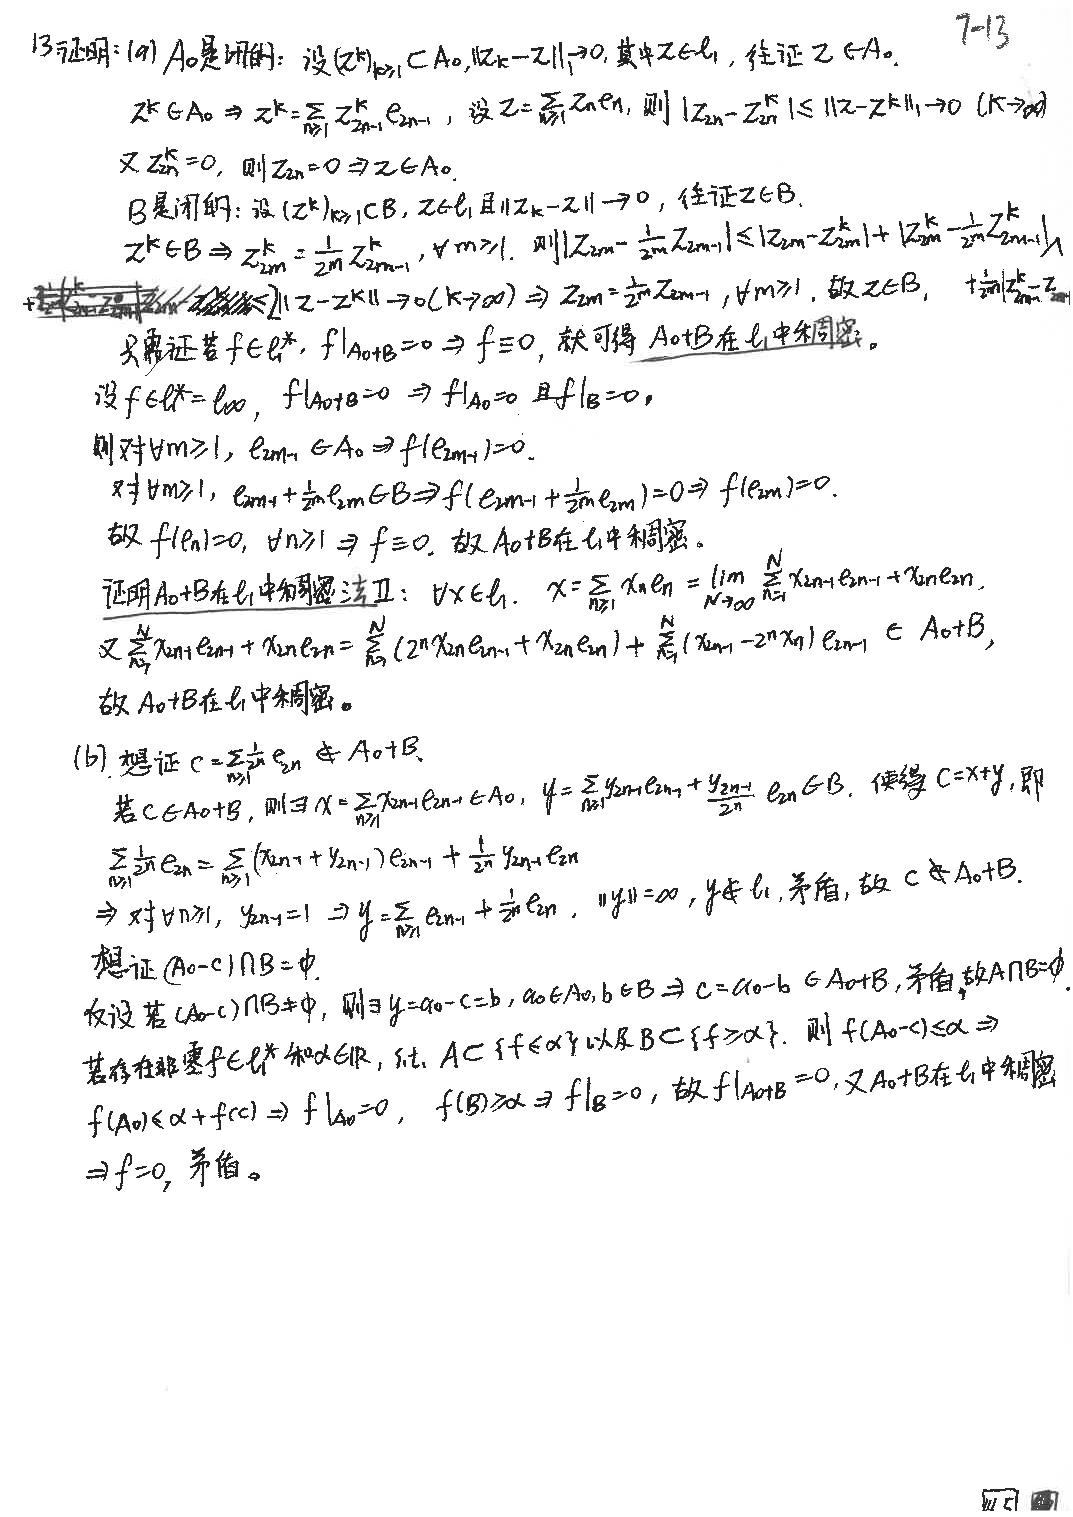
\includepdf[pages={1-1}]{7_13.pdf}
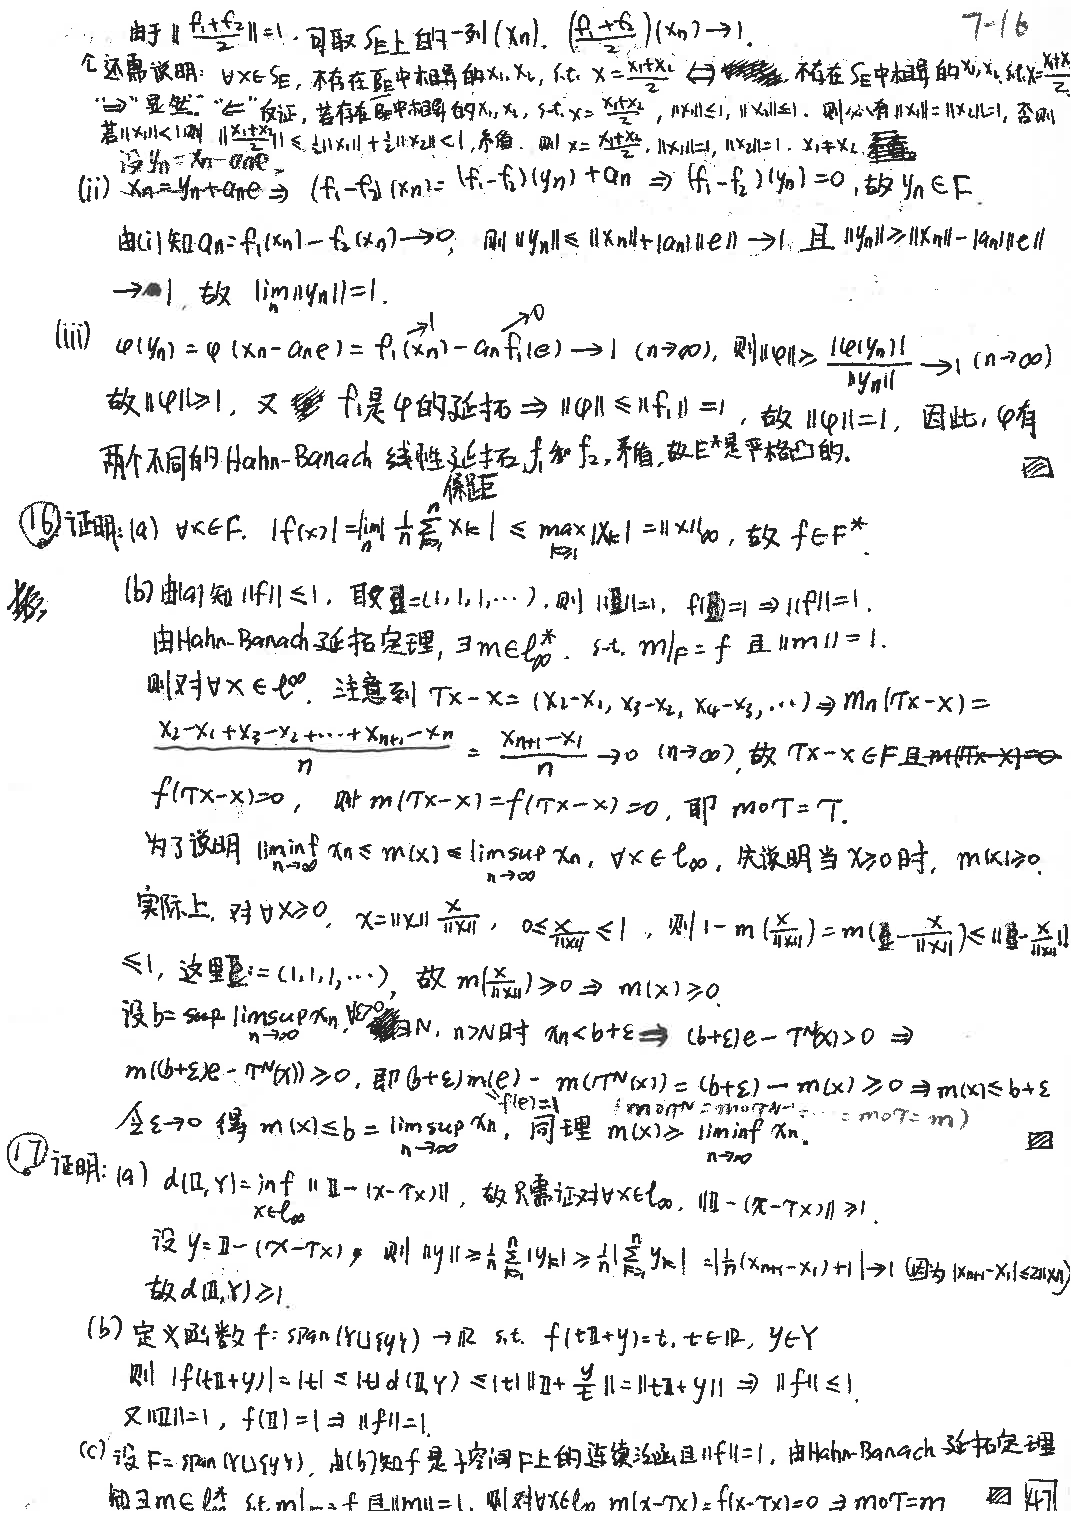
\includepdf[pages={1-1}]{7_16.pdf}
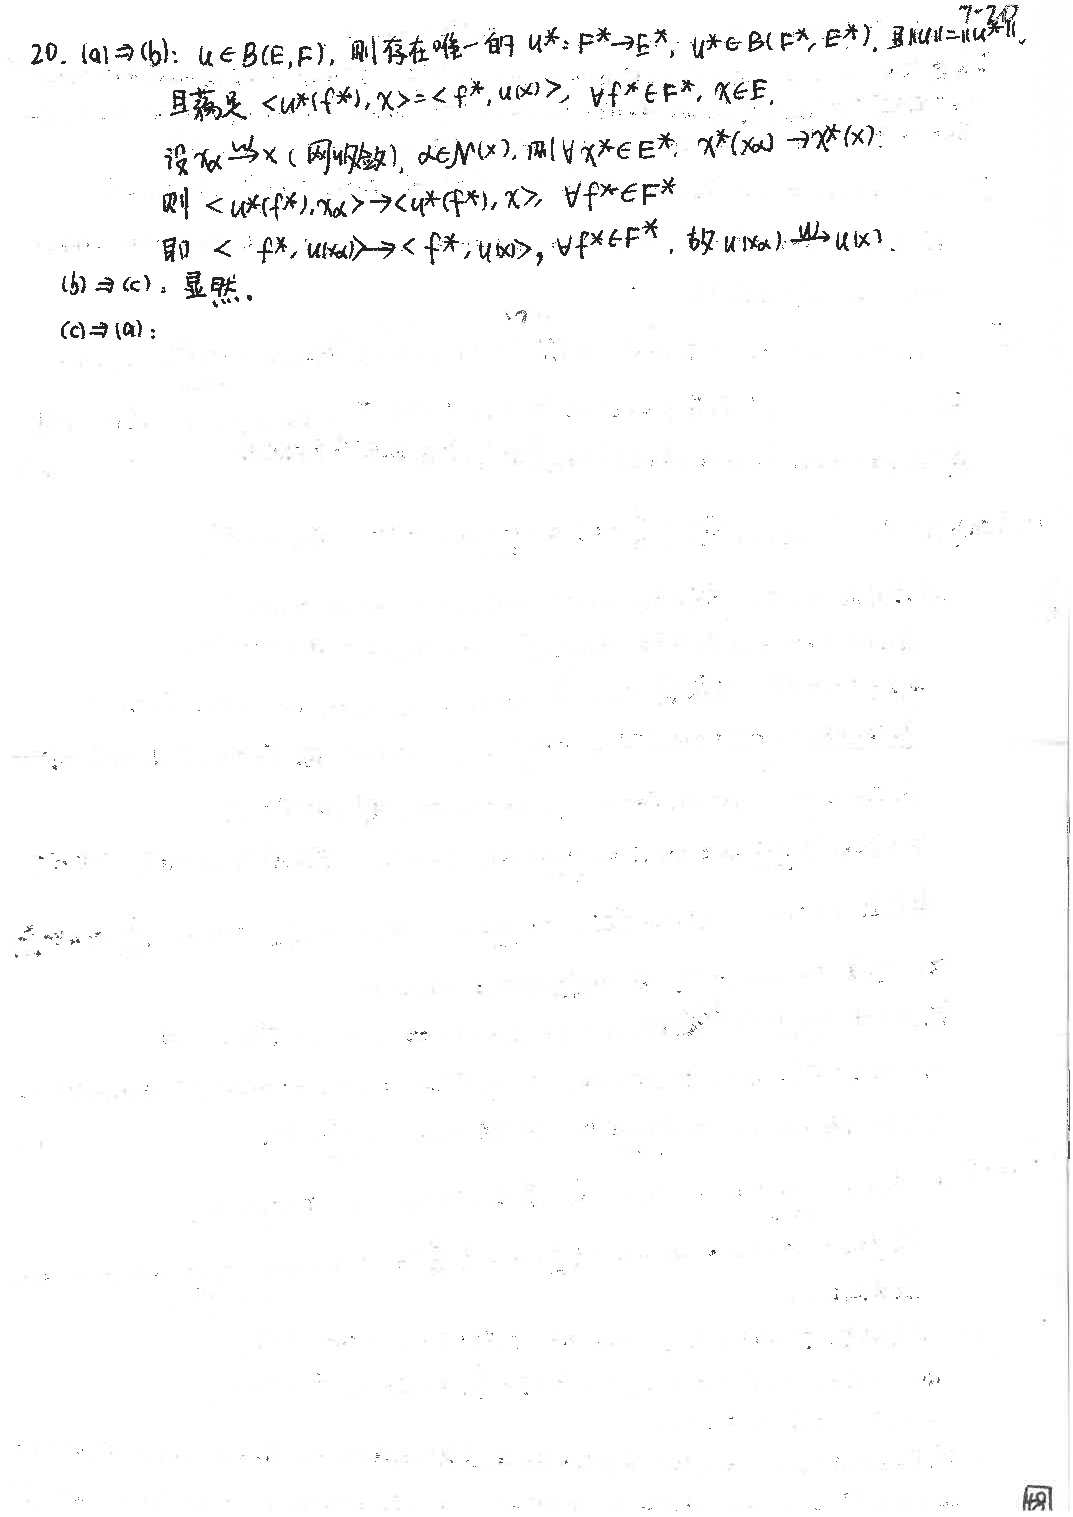
\includepdf[pages={1-1}]{7_20.pdf}
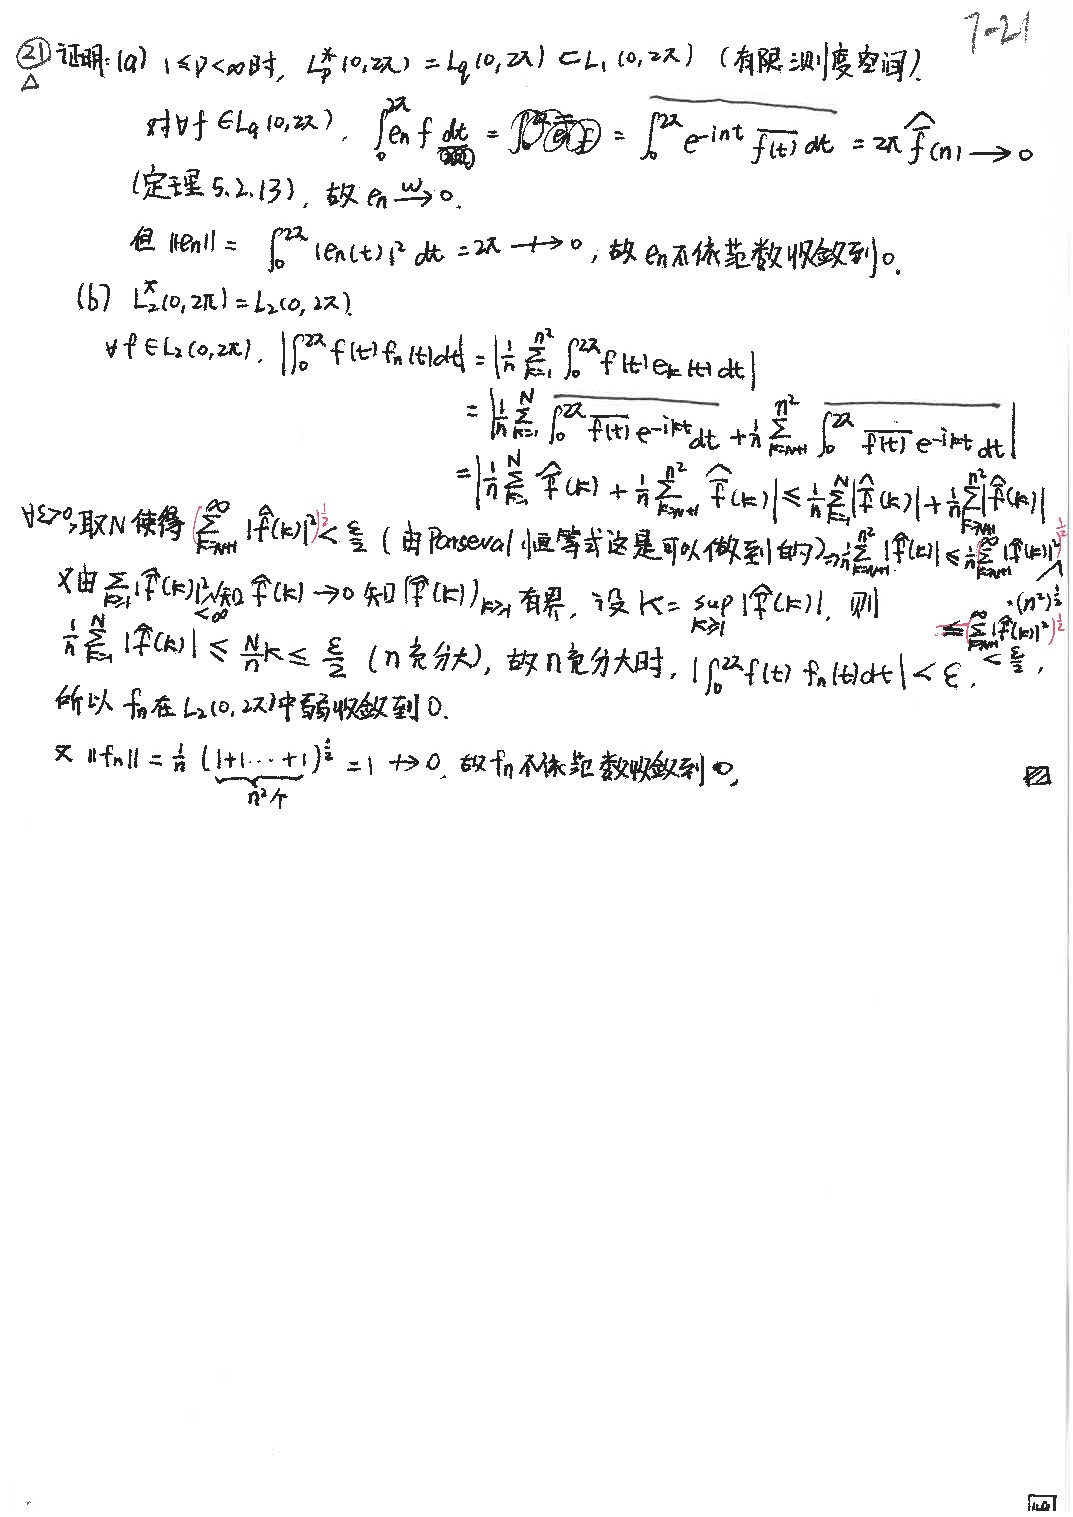
\includepdf[pages={1-1}]{7_21.pdf}
\section{第八章 习题}
1. [作业]设$1\leq p\leq\infty$, 考虑$\mathbb{R}^2$上的$p$-范数:
$$\|(x_1,x_2)\|_p=(|x_1|^p+|x_2|^p)^{\frac{1}{p}},p<\infty;\|(x_1,x_2)\|_\infty=\max\{|x_1|,|x_2|\}.$$
设$F=\mathbb{R}\times\{0\}$, 即由$e_1=(1,0)$生成的向量子空间,并设$f:F\to\mathbb{R}$是线性泛函,满足$f(e_1)=1$.
\begin{itemize}
	\item[(a)] 当$\mathbb{R}^2$上赋予$\|\cdot\|_1$范数时,确定$f$从$F$到$\mathbb{R}^2$的所有保范延拓。
	\item[(b)]当$\mathbb{R}^2$上赋予$\|\cdot\|_p$范数时,考虑同样的问题。
\end{itemize}
\begin{proof}
	(a) 设$\tilde{f}$是$f$的保范延拓,则$\|\tilde{f}\|=1$且$\tilde{f}|_F=f$. 设$e_2=(0,1)$, 则$\forall x\in\mathbb{R}^2$, $x=x_1e_1+x_2e_2$, $\tilde{f}(x_1e_1+x_2e_2)=x_1\tilde{f}(e_1)+x_2\tilde{f}(e_2)=x_1+x_2\tilde{f}(e_2)$. 设$c=\tilde{f}(e_2)$, 由$\|\tilde{f}\|=1\RA|\tilde{f}(e_2)|\leq 1\RA|c|\leq 1$. 反过来,设$|c|\leq 1$, 则易看出形如$\tilde{f}(x_1e_1+x_2e_2)=x_1+cx_2$的线性泛函为$f$的保范延拓。
	
	(b) 设$\tilde{f}$是$f$的保范延拓,则$\|\tilde{f}\|=1$且$\tilde{f}|_F=f$. 与(a)的过程一样, 只需要确定常数$c$的取值范围即可找到$f$的所有保范延拓。
	
	$1\leq p<\infty$时: 
	$$\|\tilde{f}\|=1\Leftrightarrow \frac{|x_1+cx_2|}{(|x_1|^p+|x_2|^p)^{\frac{1}{p}}}\leq 1,\forall x_1,x_2\in \mathbb{R},$$
	上式等价于$$|x_1|+|c||x_2|\leq (|x_1|^p+|x_2|^p)^{\frac{1}{p}},\forall x_1,x_2\in \mathbb{R}\Leftrightarrow |c|\leq \frac{(|x_1|^p+|x_2|^p)^{\frac{1}{p}}-|x_1|}{|x_2|}=(t^p+1)^{\frac{1}{p}}-t,\forall t\geq 0,$$
	进一步等价于$|c|\leq \inf_{t\geq 0}(t^p+1)^{\frac{1}{p}}-t$, 设$\phi(t)=(t^p+1)^{\frac{1}{p}}-t,t\geq 0$, 则$\phi(t)\geq 0$, 又由洛必达法知$\lim_{t\to\infty}\phi(t)=0$, 故$\inf_{t\geq 0}\phi(t)=0$, 因此$c=0$, $\tilde{f}(x_1e_1+x_2e_2)=x_1$即为$f$的全体保范延拓。
	
	$p=\infty$时:$\|\tilde{f}\|\leq 1\Leftrightarrow |x_1|+|c||x_2|\leq \max\{|x_1|,|x_2|\},\forall x_1,x_2\in\mathbb{R}$, 则当$|x_2|\leq|x_1|$时,$|x_1|+|c||x_2|\leq|x_1|\RA |c||x_2|\leq 0$, 取$x_2\ne 0$则$c=0$, $\tilde{f}(x_1e_1+x_2e_2)=x_1$即为$f$的全体保范延拓。
\end{proof}


3. [习题课]设$E$是数域$\mathbb{K}$上的赋范空间,$A\subset E$, 并设映射$f:A\to \mathbb{K}$以及常数$\lambda\geq 0$. 证明:存在$\hat{f}\in E^*$, 使得
$$\hat{f}|_A=f\mbox{ 且 }\|\hat{f}\|\leq\lambda$$
的充分必要条件是
\begin{equation*}
|\sum_{k=1}^n\alpha_k f(a_k)|\leq\lambda\|\sum_{k=1}^n\alpha_ka_k\|,\forall n\in\mathbb{N},\forall (a_1,\cdots,a_n)\in A^n,\forall(\alpha_1,\cdots,\alpha_n)\in\mathbb{K}^n.
\end{equation*}
\begin{proof}
	$\RA$: $|\sum_{k=1}^n\alpha_k f(a_k)|=|\hat{f}(\sum_{k=1}^n\alpha_k a_k)|\leq\lambda\|\sum_{k=1}^n\alpha_k a_k\|$.
	
	$\LA$: 记$F=\mathrm{span}(A)$, 定义$\mathrm{span}(A)$上的线性映射$\tilde{f}:\mathrm{span}(A)\to\mathbb{K}$, $\sum_{k=1}^n \alpha_k a_k\mapsto \sum_{k=1}^n\alpha_kf(a_k)$. 先验证这是良定义的:若有$\sum_{k=1}^n\alpha_k a_k=\sum_{l=1}^n \beta_lb_l$, 则
	$$|\sum_{k=1}^n\alpha_kf(a_k)-\sum_{l=1}^n\beta_lf(b_l)|\leq\lambda\|\sum_{k=1}^n\alpha_ka_k-\sum_{l=1}^n\beta_lb_l\|=0,$$
	因此$\sum_{k=1}^n\alpha_kf(a_k)=\sum_{l=1}^n\beta_lf(b_l)$, 故$\tilde{f}$是良定义的。由题设$\|\tilde{f}\|_F\leq\lambda$, 且$\tilde{f}|_A=f$, 根据Hahn-Banach定理,存在$\hat{f}\in E^*$, s.t.$\hat{f}|_F=\tilde{f}$且$\|\hat{f}\|=\|\tilde{f}\|\leq \lambda$, 所以$\hat{f}|_A=f\mbox{ 且 }\|\hat{f}\|\leq\lambda$.
\end{proof}

4. [习题课]设$E$是赋范空间(Hausdorff拓扑向量空间),$A$是$E$中包含原点的开凸集以及$x_0\in E\backslash A$.
\begin{itemize}
	\item[(a)] 证明:存在$f\in E^*$, s.t.
	\begin{equation*}
	\mathrm{Re}f(x_0)=1\mbox{且在}A\mbox{上}\mathrm{Re}f<1
	\end{equation*}
	\item[(b)] 假设$A$还是平衡的。证明:可以选择$f\in E^*$, 使其满足
	\begin{equation*}
	f(x_0)=1\mbox{且在}A\mbox{上}|f|<1
	\end{equation*}
\end{itemize}
\begin{proof}
	(a) 由于$x_0\notin A$, $\{x_0\}$是凸的,由Hahn-Banach隔离定理,存在$f\in E^*$, 常数$\alpha\in\mathbb{R}$, s.t. 
	$$\mathrm{Re}f(a)<\alpha\leq \mathrm{Re} f(x_0),\forall a\in A,$$
	由于$0\in A$, 则$\alpha>0$,  故$\mathrm{Re}f(x_0)>0$, 取$g=\frac{f}{\mathrm{Re}f(x_0)}$, 则$g\in E^*$且
	$$\mathrm{Re}g(a)=\frac{\mathrm{Re}f(a)}{\mathrm{Re}f(x_0)}<1,$$
	且$\mathrm{Re} g(x_0)=1$, $g$即为所求泛函。
	
	(b) 由于$x_0\notin A$, $\{x_0\}$是凸的,由Hahn-Banach隔离定理,存在$f\in E^*$, 常数$\alpha\in\mathbb{R}$, s.t. 
	$$\mathrm{Re}f(a)<\alpha\leq \mathrm{Re} f(x_0)\leq|f(x_0)|=\lambda f(x_0),\forall a\in A,$$
	这里$\lambda=\frac{\overline{f(x_0)}}{|f(x_0)|}$, 
	令$h=\frac{\lambda f}{|f(x_0)|}$, 则$h\in E^*$且$h(x_0)=1$, 又因为$A$平衡,故对任意$a\in A$有
	$$|h(a)|=\lambda_ah(a)=\frac{\lambda_a \lambda f(a)}{|f(x_0)|}=\frac{f(\lambda_a\lambda a)}{|f(x_0)|}=\frac{\mathrm{Re} f(\lambda_a\lambda a)}{|f(x_0)|}<\frac{|f(x_0)|}{|f(x_0)|}=1,$$
	其中$\lambda_a=\frac{\overline{h(a)}}{|h(a)|}$, 故$h$即为所求泛函。
\end{proof}

5. [作业]设$E$是赋范空间(Hausdorff局部凸空间),$A$是$E$中包含原点的闭凸集以及$x_0\in E\backslash A$.
\begin{itemize}
	\item[(a)] 证明:存在$f\in E^*$, 使得
	$$\mathrm{Re} f(x_0)>1\mbox{且}\sup_{x\in A}\mathrm{Re} f(x)\leq 1.$$
	\item[(b)] 假设$A$还是平衡的。证明: 可以选择$f$, 使其满足
	$$f(x_0)>1\mbox{且}\sup_{x\in A}|f(x)|\leq 1.$$
\end{itemize}
\begin{proof}
	(a) 由Hahn-Banach严格隔离定理,存在$g\in E^*,\alpha,\beta\in\mathbb{R}$, 使得
	$$\sup_{x\in A}\mathrm{Re}g(x)<\alpha<\beta<\Re g(x_0),$$
	又显然$0\in A$, 则$0<\alpha<\beta$, 令$f=\frac{g}{\alpha}$那么$\Re f(x_0)>1$且$\sup_{x\in A}\Re f(x)<1$.
	
	(b) 由Hahn-Banach严格隔离定理,存在$g\in E^*,\alpha,\beta\in\mathbb{R}$, 使得
	$$\sup_{x\in A}\mathrm{Re}g(x)<\alpha<\beta<\Re g(x_0)\leq|g(x_0)|=\lambda g(x_0),$$
	其中$\lambda=\frac{\overline{g(x_0)}}{|g(x_0)|}$, 令$f=\frac{\lambda g}{\alpha}$, 则$f(x_0)=\frac{|g(x_0)|}{\alpha}>1$, 且由于$A$是均衡的,
	$$\sup_{a\in A}|f(a)|=\sup_{a\in A}\Re f(a)=\frac{1}{\alpha}\sup_{a\in A}\Re \lambda g(a)=\frac{1}{\alpha}\sup_{a\in A}\Re g(\lambda a)=\frac{1}{\alpha}\sup_{a\in A}\Re g(a)<1.$$
\end{proof}


6. [作业]设$E$是实的赋范空间(Hausdorff局部凸空间),$A\subset E$. 定义$E$的子集$\hat{A}$由满足如下性质的元素$x$构成:若取$f\in E^*$满足对任意$a\in A$, 有$f(a)\leq 1$, 则$f(x)\leq 1$. 
\begin{itemize}
	\item[(a)] 证明:$\overline{\mathrm{conv}(A)}\subset \hat{A}$.
	\item[(b)] 证明:$\overline{\mathrm{conv}(A)}=\hat{A}$等价于$0\in\overline{\mathrm{conv}(A)}$.
\end{itemize}
\begin{proof}
	(a) 注意到$A\subset\hat{A}$, 故只需验证$\hat{A}$是凸的且闭的。设$x\in \hat{A}$, $y\in\hat{A}$, 若$f\in E^*$满足对于任意$a\in A$, $f(a)\leq 1$, 则$f(x)\leq 1$, $f(y)\leq 1$, 那么$f(\lambda x+(1-\lambda)y)\leq \lambda f(x)+(1-\lambda)f(y)\leq 1\RA \lambda x+(1-\lambda)y\in\hat{A}$, 故$\hat{A}$是凸的,则$\mathrm{conv}(A)\subset\hat{A}$. 
	
	设$(x_n)_{n\geq 1}\subset \hat{A}$, 且收敛于某个$x$, 若$f\in E^*$满足对于任意$a\in A$, $f(a)\leq 1$, 则$f(x_n)\leq 1$, 由$f$连续,令$n\to\infty$得$f(x)\leq 1$, 故$x\in\hat{A}$, 所以$\hat{A}$是闭的。
	
	(b)"$\RA$": 显然$0\in\hat{A}$, 因此$0\in\overline{\mathrm{conv}(A)}$.
	
	"$\LA$": 反证法,
	若$\overline{\mathrm{conv}(A)}\ne \hat{A}$, 则$\overline{\mathrm{conv}(A)}\subsetneq \hat{A}$, 那么存在$x_0\in \hat{A}$, $x_0\notin\overline{\mathrm{conv}(A)}$, 由习题5(a)(这里$E$是实数域上的,那里的$\Re f$可以直接换成$f$)知存在$f\in E^*$, $$f(a)\leq 1,\forall a\in \overline{\mathrm{conv}(A)}\mbox{且}f(x_0)>1,$$ 这与$x_0\in \hat{A}$矛盾,故$\overline{\mathrm{conv}(A)}=\hat{A}$.
\end{proof}

7. [习题课]设$E$是赋范空间(Hausdorff局部凸空间),$A\subset E$. 定义$E$的子集$\hat{A}$由满足如下性质的元素$x$构成:若取$f\in E^*$满足对任意$a\in A$, 有$|f(a)|\leq 1$, 则$|f(x)|\leq 1$. 

设$\mathrm{ccb}A$表示$A$的闭凸平衡包,即包含$A$的所有闭凸平衡集的交集。
\begin{itemize}
	\item[(a)] 证明:$\mathrm{ccb} A\subset \hat{A}$.
	\item[(b)] 证明:$\mathrm{ccb}A=\hat{A}$.
\end{itemize}
\begin{proof}
	(a) 注意到$A\subset\hat{A}$, 故只需验证$\hat{A}$是闭凸平衡集。设$x\in \hat{A}$, $y\in\hat{A}$, 若$f\in E^*$满足对于任意$a\in A$, $|f(a)|\leq 1$, 则$|f(x)|\leq 1$, $|f(y)|\leq 1$, 那么$|f(\lambda x+(1-\lambda)y)|\leq \lambda|f(x)|+(1-\lambda)|f(y)|\leq 1$, 故$\hat{A}$是凸的,同理可证$\hat{A}$是平衡的。设$(x_n)_{n\geq 1}\subset \hat{A}$, 且收敛于某个$x$, 若$f\in E^*$满足对于任意$a\in A$, $|f(a)|\leq 1$, 则$|f(x_n)|\leq 1$, 令$n\to\infty$得$|f(x)|\leq 1$, 故$x\in \hat{A}$, 故$\hat{A}$是闭的。
	
	(b)
	若$\mathrm{ccb}A\ne \hat{A}$, 则$\mathrm{ccb}A\subsetneq \hat{A}$, 那么存在$x_0\in \hat{A}$, $x_0\notin\mathrm{ccb}A$, 由习题5(b)知存在$f\in E^*$, $|f(a)|\leq 1,\forall a\in \mathrm{ccb}A$且$f(x_0)>1$, 这与$x_0\in \hat{A}$矛盾。
\end{proof}

9. [习题课]设$E$是数域$\mathbb{K}$上的赋范空间(拓扑向量空间)。称$E$的向量子空间$H$是超平面,若有某个$x_0\in E\backslash H$, 使得$E=H+\mathbb{K}x_0$.
\begin{itemize}
	\item[(a)] 证明:若$H$是超平面,则对任意$x_0\in E\backslash H$, $E=H+\mathbb{K}x_0$成立。
	\item[(b)] 证明:一个超平面或是$E$中的稠密集,或是闭集。
	\item[(c)] 证明:$H$是超平面当且仅当存在$E$上的一个非零线性泛函$f$, 使得$H=\ker f$. 因而$H$是闭的等价于$f$是连续的。
\end{itemize}
\begin{proof}
	(a) $H$是超平面,则存在$x\in E\backslash H$, s.t. $E=H+\mathbb{K}x$. 对任意$x_0\notin H$, $x_0=h+\lambda x$, 则$\lambda\ne 0$, 故$x=\frac{x_0-h}{\lambda}\in H+\mathbb{K}x_0$, 所以$E=H+\mathbb{K}x\subset H+\mathbb{K}x_0\RA E=H+\mathbb{K}x_0$.
	
	(b) 设$H$是超平面,则存在$x_0\in E\backslash H$, 使得$E=H+\mathbb{K}x_0$. 若$x_0\in\overline{H}$, 则$E=H+\mathbb{K}x_0\subset \overline{H}$, 
	故$E=\overline{H}$. 
	
	若$x_0\notin \overline{H}$, 则由Hahn-Banach延拓定理,存在$f\in E^*$, $f|_H=0$, 但$f(x_0)\ne 0$, 那么$H\subset \ker(f)$. 又对于任意$x\in E$, $x=h+\alpha x_0$, $h\in H, \alpha\in \mathbb{K}$, 故
	$$f(x)=0\RA f(h+\alpha x_0)=f(h)+\alpha f(x_0)=0,$$ 注意到$f(h)=0$, 故$\alpha=0$, 这意味着$\ker f\subset H$, 因此$H=\ker f$, 故$H$是闭的。
	
	法II: 若$H$是稠密的,不需要再说明什么。
	
	若$H$不稠密,只需证明$H$一定是闭的。反证法,假设$H$不是闭的,则存在$H$中某个序列$(x_n)$收敛于某个$x\in E\backslash H$, 则$d(x,H)=0$且$E=H+\mathbb{K}x$. 对于任意$y\in E\backslash H$, 存在$h_0\in H$, $\alpha\in \mathbb{K}\backslash \{0\}$使得$y=h_0+\alpha x$, 则 \[d(y,H)=\inf \{\|y-h\|: h\in H\}=\inf \{\|h_0+\alpha x-h\|: h\in H\}=|\alpha|\inf \{\|x-h\|: h\in H\}=0,\]
	故$y\in \overline{H}$, 那么$H$在$E$中稠密,矛盾,故$H$是闭的。
	
	(c) $\LA$: 设存在$E$上的非零线性泛函$f$, s.t. $H=\ker f$, 由于存在$x_0\in E$, s.t.$f(x_0)\ne 0$, 因此$x_0\notin H$. 对任意$e\in E$, $$e=e-\frac{f(e)}{f(x_0)}x_0+\frac{f(e)}{f(x_0)}x_0\in H+\mathbb{K}x_0,$$
	故$H$是超平面。若$f$还是连续的,则$H=\ker f$是闭的。
	
	$\RA$: 设$H$是超平面,则存在$x_0\in E\backslash H$, 使得$E=H+\mathbb{K}x_0$. 则任意$x\in E$可写为$x=h+\alpha x_0$, 定义$E$上的线性泛函$f$为$f(h+\alpha x_0)=\alpha$, 则$H=\ker f$, 且$f(x_0)=1\RA f$非零。
	
	若$H=\ker f$还是闭的,想证明$f$连续。反证法,若$f$不连续,则存在$(x_n)_{n\geq 1},\|x_n\|=1$, 且$|f(x_n)|\geq n$. 令$y_n=\frac{x_n}{f(x_n)}-\frac{x_1}{f(x_1)}$, 则$f(y_n)=0$, 即$y_n\in \ker f$, 但是$y_n\to\frac{x_1}{-f(x_1)}\notin\ker f$, 故$\ker f$不是闭的,矛盾。
	
	第二种由$\ker f$闭推出$f$连续的方法:若$H=\ker f$是闭的,我们取线性泛函
	$$\tilde{f}(h+\alpha x_0)=\alpha d(x_0,F),$$ 则$\tilde{f}$是连续的,则$f(h+\alpha x_0)=\alpha=\frac{1}{d(x_0,F)}\alpha d(x_0,F)=\frac{1}{d(x_0,F)}\tilde{f}(h+\alpha x_0)$连续。
\end{proof}
\begin{Remark}
	设$f:X\to Y$是一般的赋范空间之间的线性映射,$\ker f$闭一般推不出$f$连续,比如第六章习题16给出的线性映射$u$, $\ker u=\mathbb{K}$有限维所以是闭的,但$u$不连续。特别地,$X=Y$时也有反例,参见《泛函分析中的反例》77页。
\end{Remark}

13. 考虑空间$\ell_1$中的如下子集:
\[\begin{split}
A_0=&\{x=(x_n)_{n\geq 1}\in\ell_1:x_{2n}=0,\forall n\geq 1\},\\
B=&\{x=(x_n)_{n\geq 1}\in\ell_1:x_{2n}=2^{-n}x_{2n-1},\forall n\geq 1\}.
\end{split}\]
\begin{itemize}
	\item[(a)] 证明:$A_0$和$B$是$\ell_1$的闭向量子空间且$A_0+B$在$\ell_1$中稠密。
	\item[(b)] 设$c\in\ell_1$满足$c_{2n-1}=0$及$c_{2n}=2^{-n}$, 并设$A=A_0-c$. 证明:$c\notin A_0+B$且$A\cap B=\varnothing$. 并证明:不存在非零的$f\in\ell_1^*$和$\alpha\in\mathbb{R}$, 使得$A\subset\{f\leq \alpha\}$以及$B\subset\{f\geq \alpha\}$.
\end{itemize}
\begin{proof}
	(a) 在$\ell_1$中依范数收敛则逐点收敛:设$(z^k)_{k\geq 1}\subset \ell_1$收敛于$z\in \ell_1$, 则对任意$n\geq 1$有
	$|z_n^k-z_n|\leq\|z^k-z\|_1\to 0(k\to\infty).$
	
	$A_0$闭:设$(z^k)_{k\geq 1}\subset A_0$收敛于$z\in \ell_1$, 则对任意$n\geq 1$有$z_{2n}=\lim_{k\to\infty} z_{2n}^k=0$, 故$z\in A_0$.
	
	$B$闭:设$(z^k)_{k\geq 1}\subset B$收敛于$z\in \ell_1$, 则对任意$n\geq 1$有$z_{2n}=\lim_{k\to\infty} z_{2n}^k=\lim_{k\to\infty}\frac{1}{2^n}z_{2n-1}^k=\frac{1}{2^n}z_{2n-1}$, 故$z\in B$.
	
	只需证明若$f\in\ell_1^*$, $f|_{A_0+B}=0$时$f \equiv 0$, 就可得$A_0+B$在$\ell_1$中稠密:设$f\in\ell_1^*$, $f|_{A_0+B}=0$则$f|_{A_0}=0$且$f|_{B}=0$则对任意$m\geq 1$, $f(e_{2m-1})=0$且$f(e_{2m}+2^me_{2m-1})=0$, 所以$f(e_{2m})=0$, 故$f(e_n)=0,\forall n\geq 1$, 即$f\equiv 0$, 故$A_0+B$在$\ell_1$中稠密
	
	法II:$\forall x\in\ell_1$, 
	\[\begin{split}
	x=\sum_{n\geq 1}x_ne_n=&\lim_{N\to\infty}\sum_{n=1}^Nx_{2n-1}e_{2n-1}+x_{2n}e_{2n}\\
	=&\lim_{N\to\infty}\sum_{n=1}^N(2^nx_{2n}e_{2n-1}+x_{2n}e_{2n})+\sum_{n=1}^N(x_{2n-1}-2^nx_n)e_{2n-1}\in \overline{A_0+B},
	\end{split}\]
	故$A_0+B$在$\ell_1$中稠密。
	
	(b) 先证明$c\notin A_0+B$: 反证法,若$c\in A_0+B$, 则存在$x=\sum_{n\geq 1}x_{2n-1}e_{2n-1}\in A_0$, $y=\sum_{n\geq 1}y_{2n-1}e_{2n-1}+\frac{y_{2n-1}}{2^n}e_{2n}\in B$使得
	\[c=x+y=\sum_{n\geq 1}2^{-n}e_{2n}=\sum_{n\geq 1}(x_{2n-1}+y_{2n-1})e_{2n-1}+\frac{1}{2^n}y_{2n-1}e_{2n},\]
	则对任意$n\geq 1$, $y_{2n-1}=1$, 这意味着$\|y\|=\infty$, 这与$y\in\ell_1$矛盾,所以$x\notin A_0+B$.
	
	再证$(A_0-c)\cap B=\varnothing$: 反证,若$(A_0-c)\cap B\ne\varnothing$, 则存在$a_0\in A_0,b\in B$使得$a_0-c=b$, 故$c=a_0-b\in A_0+B$, 矛盾,故$A\cap B=\varnothing$.
	
	若存在非零$f\in\ell_1^*$和$\alpha\in\mathbb{R}$, 使得$A\subset \{f\leq\alpha\}$且$B\subset\{f\geq \alpha\}$, 则由于$A_0$与$B$是线性空间则
	\[f(A_0-c)\leq\alpha\RA f(A_0)\leq\alpha+f(c)\RA f|_{A_0}=0,\]
	\[f(B)\geq \alpha\RA f|_{B}=0,\]
	故$f|_{A_0+B}=0$, 又$A_0+B$在$\ell_1$中稠密,则$f\equiv0$, 矛盾。
\end{proof}

15. 设$E$是一个维数至少为2的赋范空间,证明: $E$的向量子空间$F$上每个连续线性泛函有唯一的保范延拓当且仅当$E^*$是严格凸的。我们称一个赋范空间$E$是严格凸的,若其单位球面$S_E$上的每个点是其闭单位球$\overline{B}_E$上的端点。
\begin{proof}
	首先说明:对任意赋范空间$E$, $E$严格凸等价于: $\forall x\in S_E$, 不存在$S_E$中相异两点$x_1,x_2$, 使得$x=\frac{x_1+x_2}{2}$. "$\RA$", 显然; "$\LA$", 反证法,假设$E$不严格凸,则存在$x\in S_E$与$\overline{B}_E$中相异的两点$x_1,x_2$, s.t.$x=\frac{x_1+x_2}{2}$, 则必有$\|x_1\|=\|x_2\|=1$(否则若$\|x_1\|<1$, 则$\|\frac{x_1+x_2}{2}\|\leq\frac{1}{2}\|x_1\|+\frac{1}{2}\|x_2\|<1$, 矛盾), 这与我们的条件矛盾。
	
	(a) "$\LA$": 反证法,反设存在$F$上某个连续泛函$f\in F^*$有两个不同的保范延拓$\tilde{f_1},\tilde{f_2}\in E^*$, 不妨设$\|f\|=1$,  则$\tilde{f_1}|_F=\tilde{f_2}|_F=f$且$\|\tilde{f_1}\|=\|\tilde{f_2}\|=1$. 令$\tilde{f}=\frac{\tilde{f_1}+\tilde{f_2}}{2}$, 则$\tilde{f}\in E^*$, $\tilde{f}|_F=f$且$\|\tilde{f}\|\leq\frac{1}{2}(\|\tilde{f_1}\|+\|\tilde{f_2}\|)=1$, 则必有$\|\tilde{f}\|<1$(否则若$\|\tilde{f}\|=1$则会与$E^*$严格凸矛盾)。然而$\tilde{f}$是$f$的保范延拓$\RA\|\tilde{f}\|\geq\|f\|=1$, 矛盾,所以$\tilde{f_1}=\tilde{f_2}$.
	
	(b)"$\RA$": 反证法,反设$E^*$不是严格凸的,则存在$f\in S_{E^*}$, 可以写成$f=\frac{f_1+f_2}{2}$, 其中$\|f_1\|=\|f_2\|=1,f_1\ne f_2$. 由于$\|\frac{f_1+f_2}{2}\|=1$, 可取一列$(x_n)_{n\geq 1},\|x_n\|=1$且$\left(\frac{f_1+f_2}{2}\right)(x_n)\to 1$. 
	
	想说明$\lim_{n\to\infty}f_1(x_n)=\lim_{n\to\infty}f_2(x_n)=1$. 已知$|f_1(x_n)|\leq\|f_1\|\|x_n\|\leq 1$, 同理$|f_2(x_n)|\leq 1$, 
	则
	\begin{equation*}
	(f_1(x_n)+f_2(x_n))-1\leq f_1(x_n)+f_2(x_n)-f_2(x_n)=f_1(x_n)\leq 1,
	\end{equation*} 
	由两边夹定理知$(f_1(x_n))$极限存在且$\lim_{n\to\infty}f_1(x_n)=1$, 则$\lim_{n\to\infty}f_2(x_n)=1$. 
	
	设$F=\ker(f_1-f_2)$且$\phi$是$f_1$在$F$上的限制,则$\phi$也是$f_2$在$F$上的限制,想说明$\|\phi\|=1$. 由于$f_1\ne f_2$, 可取适当的$e$使得$(f_1-f_2)(e)=1$, 设$y_n=x_n-a_ne$, 其中$a_n=(f_1-f_2)(x_n)\to 0(n\to\infty)$. 由于$(f_1-f_2)(y_n)=0$, 则$y_n\in F$, 又
	$$\|x_n\|-|a_n|\|e\|\leq \|y_n\|\leq \|x_n\|+|a_n|\|e\|,$$
	令$n\to\infty$知$\lim_{n\to\infty}\|y_n\|=1$.  
	
	注意到$\phi(y_n)=\phi(x_n-a_ne)=f_1(x_n)-a_nf_1(e)\to 1(n\to\infty)$, 则$\|\phi\|\geq \frac{|\phi(y_n)|}{\|y_n\|}\to 1(n\to\infty)\RA \|\phi\|\geq 1$, 又因为$f_1$是$\phi$的延拓$\RA\|\phi\|\leq\|f_1\|=1$, 故$\|\phi\|=1$, 因此$\phi$有两个不同的保范延拓$f_1$和$f_2$, 矛盾,故$E^*$是严格凸的。
\end{proof}

16. 考虑空间$\ell_{\infty}$和它的向量子空间$F$:
\[F=\{x\in\ell_{\infty}:\lim_{n\to\infty}m_n(x)\text{ 存在}\}, \text{ 其中 }m_n(x)=\frac{1}{n}\sum_{k=1}^n x_k.\]
\begin{itemize}
	\item[(a)] 定义$f:F\to\mathbb{R}$为$f(x)=\lim_{n\to\infty}m_n(x)$. 证明:$f\in F^*$.
	\item[(b)] 证明:存在$\ell_{\infty}$上连续线性泛函$m$满足下面的性质:
	
	(i)$\liminf_{n\to\infty}x_n\leq m(x)\leq \limsup_{n\to\infty} x_n$, $\forall x\in \ell_{\infty}$.
	
	(ii)$m\circ \tau=m$, 这里$\tau:\ell_{\infty}\to\ell_{\infty}$是右移算子,即$\tau(x)_{n}=x_{n+1}$. ($m$被称为Banach平均或$\ell_{\infty}$极限.)
\end{itemize}
\begin{proof}
	(a) $\forall x\in F$, $|f(x)|\leq \lim_{n}|\frac{1}{n}\sum_{k=1}^nx_k|\leq \max_{k\geq 1}|x_k|=\|x\|_{\infty}$, 故$f\in F^*$.
	
	(b) 由(a)知道$\|f\|\leq 1$, 取定$\mathbb{I}=(1,1,1,\cdots)$, 则$\|\mathbb{I}\|=1$且$f(\mathbb{I})=1$, 因此$\|f\|=1$. 由Hahn-Banach延拓定理,存在$m\in \ell_{\infty}^*$, s.t. $m|_{F}=f$且$\|m\|=1$. 对任意$x\in \ell_{\infty}$, 注意到
	\[\tau x-x=(x_2-x_1,x_3-x_2,\cdots),\]
	则$m_n(\tau x-x)=\frac{x_n-x_1}{n}\to 0(n\to\infty)$, 故$\tau x-x\in F$且$f(\tau x-x)=0$, 则$m(\tau x-x)=f(\tau x-x)=0$, 即$m\circ \tau=m$.
	
	先说明当$x\geq 0$($x\geq y$即$x_i\geq y_i,\forall i\geq 1$)时$m(x)\geq 0$: 对任意$x\geq 0$, $x=\|x\|\frac{x}{\|x\|}$, $0\leq \frac{x}{\|x\|}\leq 1$, 则
	\[1-m(\frac{x}{\|x\|})=m(\mathbb{I}-\frac{x}{\|x\|})\leq \|\mathbb{I}-\frac{x}{\|x\|}\|\leq 1,\]
	故$m(\frac{x}{\|x\|})\geq 0$, 则$m(x)\geq 0$.
	
	设$b=\limsup_{n\to\infty} x_n$, 则对任意$\e>0$, 存在$N\geq 1$, 当$n>N$时
	\[x_n<b+\e\Rightarrow(b+\e)\mathbb{I}-\tau^{N}x>0\RA m((b+\e)\mathbb{I}-\tau^{N}(x))\geq 0\]
	又由于$m\circ \tau=m\RA m\circ \tau^N=m$, 则$m(x)\leq b+\e$, 由$\e$的任意性得$m(x)\leq b=\limsup_{n\to\infty}x_n$, 同理$m(x)\geq \liminf_{n\to\infty}x_n$.
\end{proof}

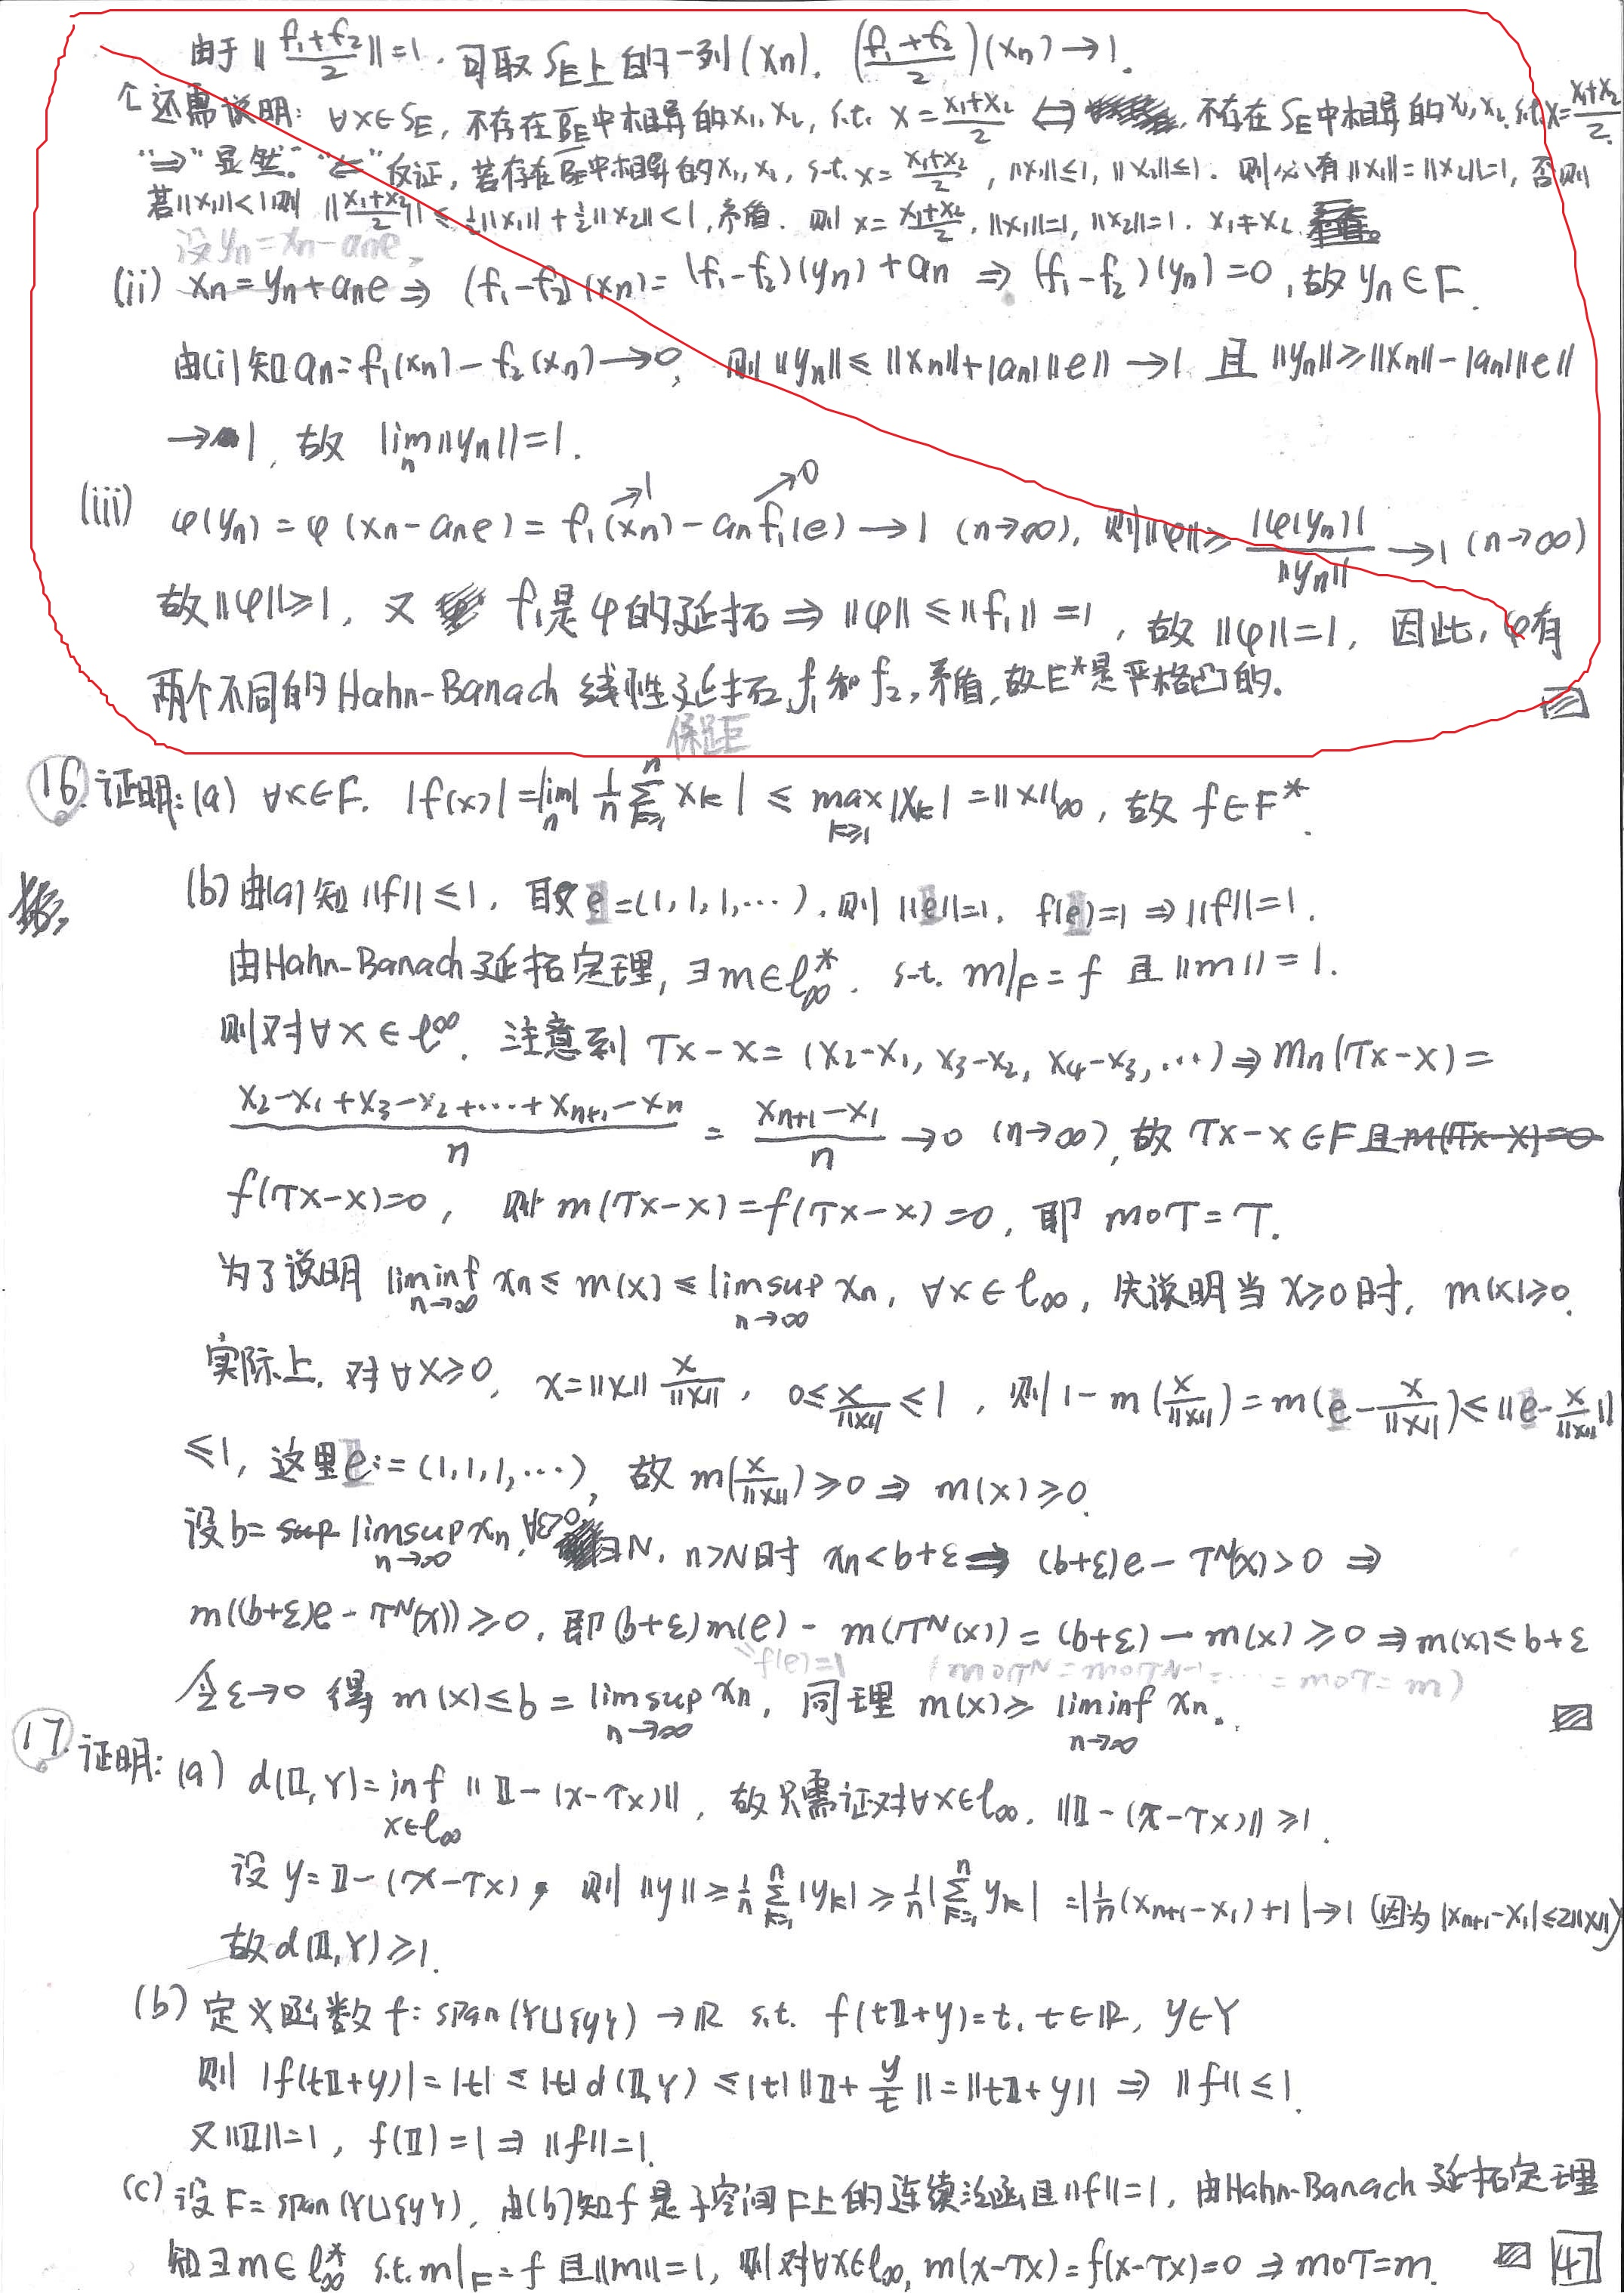
\includegraphics[scale=0.8]{9_16.jpg}
\clearpage

21. 设$e_n(t)=e^{int},t\in[0,2\pi]$.
\begin{itemize}
	\item[(a)] 证明:对每个$1\leq p<\infty$, $e_n$在$L_p(0,2\pi)$中弱收敛到$0$但不依范数收敛到$0$.
	\item[(b)] 设$f_n=\frac{1}{n}\sum_{k=1}^{n^2}e_k$. 证明:$f_n$在$L_2(0,2\pi)$中弱收敛到$0$但不依范数收敛到$0$.
\end{itemize}
\begin{proof}
	(a) $1\leq p<\infty$时,$L_p^*(0,2\pi)=L_q(0,2\pi)\subset L_1(0,2\pi)$(有限测度空间)。由于Fourier变换把$L_1(0,2\pi)$中的元素映射到$c_0$, 则对$\forall f\in L_1(0,2\pi)$, 有
	\begin{equation*}
	\int_0^{2\pi} e_n(t)f(t)dt=\overline{\int_0^{2\pi}e^{-int}\overline{f(t)}dt}=2\pi\hat{\overline{f}}(n)\to 0
	\end{equation*}
	所以$e_n\stackrel{w}{\to} 0$. 
	
	$\|e_n\|=|\int_0^{2\pi}|e_n(t)|^pdt|^{\frac{1}{p}}=(2\pi)^{\frac{1}{p}}\nrightarrow 0$, 故$e_n$不依范数收敛到0.
	
	(b)$L_2^*(0,2\pi)=L_2(0,2\pi)$. 对任意$f\in L_2(0,2\pi)$, 
	\begin{equation*}
	\begin{split}
	|\int_0^{2\pi}f(t)f_n(t)dt|=&|\frac{1}{n}\sum_{k=1}^{n^2}f(t)e_k(t)dt|\\
	=&\left|\frac{1}{n}\sum_{k=1}^N\overline{\int_{0}^{2\pi}\overline{f(t)}e^{-ikt}dt}+\frac{1}{n}\sum_{k=N+1}^{n^2}\overline{\int_{0}^{2\pi}\overline{f(t)}e^{-ikt}dt}\right|\\
	=&\left|\frac{1}{n}\sum_{k=1}^N\hat{\overline{f}}(k)+\frac{1}{n}\sum_{k=N+1}^{n^2}\hat{\overline{f}}(k)\right|\leq \frac{1}{n}\sum_{k=1}^N|\hat{\overline{f}}(k)|+\frac{1}{n}\sum_{k=N+1}^{n^2}|\hat{\overline{f}}(k)|,
	\end{split}
	\end{equation*}
	由Parseval恒等式知,对$\forall \e>0$, 可取$N$使得$(\sum_{k=N+1}^{\infty}|\hat{\overline{f}}(k)|^2)^{\frac{1}{2}}<\frac{\e}{2}$, 因此
	$$\frac{1}{n}\sum_{k=N+1}^{n^2}|\hat{\overline{f}}(k)|\leq \frac{1}{n}(\sum_{k=N+1}^{n^2}|\hat{\overline{f}}(k)|^2)^{\frac{1}{2}}\cdot(n^2)^{\frac{1}{2}}\leq(\sum_{k=N+1}^{\infty}|\hat{\overline{f}}(k)|^2)^{\frac{1}{2}}<\frac{\e}{2},$$
	又由Parseval恒等式知$\hat{\overline{f}}(k)\to 0(k\to\infty)$知$(\hat{\overline{f}}(k))_{k\geq 1}$有界,设$K=\sup_{k\geq 1}|\hat{\overline{f}}(k)|$, 则$n$充分大时,
	$$\frac{1}{n}\sum_{k=1}^N|\hat{\overline{f}}(k)|\leq \frac{N}{n}K<\frac{\e}{2},$$
	因此$n$充分大时有$|\int_0^{2\pi}f(t)f_n(t)dt|<\e$, 所以$f_n$在$L_2(0,2\pi)$中弱收敛到$0$. 
	
	$\|f_n\|=\frac{\sqrt{2\pi}}{n}(1+1+\cdots+1)^{\frac{1}{2}}=\sqrt{2\pi}\nrightarrow0$.
\end{proof}

\section{第九章 习题}
1. 设$E$是赋范空间,并设$E^*$是可分的。
\begin{itemize}
	\item[(a)] 令$(f_n)$是$E^*$中的稠密子集,选出$E$中的序列$(x_n)$使得$f_n(x_n)\geq \frac{\|f_n\|}{2}$且$\|x_n\|= 1$.
	\item[(b)] 任取$f\in E^*$. 证明:若对每个$x_n$有$f(x_n)=0$, 则$f=0$.
	\item[(c)] 由此导出$\mathrm{span}(x_1,x_2,\cdots)$在$E$中稠密且$E$是可分的。
	\item[(d)] 证明:一个Banach空间是可分的且自反的当且仅当它的对偶空间是可分的且自反的。
	\item[(e)] 举一个可分赋范空间但其对偶空间不可分的例子。
\end{itemize}
\begin{proof}
	(a) $E^*$是可分的,则存在一列$(f_n)\subset E^*$中的稠密子集,即$\overline{(f_n)}=E^*$.  由$\|f_n\|=\sup_{\|x\|=1}|f_n(x)|$, 则对任意$n\geq 1$, 存在$x_n$, $\|x_n\|=1$且$\|f_n(x_n)\|\geq \frac{\|f_n\|}{2}$. 
	
	(b) 任意$f\in E^*$, $\forall \e>0$, 存在$n\in\mathbb{N}$, $\|f-f_n\|<\e$, 则
	$$\frac{1}{2}\|f_n\|\leq |f_n(x_n)|=|(f_n-f)(x_n)|\leq|f_n-f|<\e,$$
	因此$\|f_n\|<2\e$, 则$\|f\|\leq\|f-f_n\|+\|f_n\|<3\e$, 故$f=0$.
	
	(c)设$M=\mathrm{span}(x_n)$我们已经证明了$f|_M=0\Rightarrow f=0$. 故$\mathrm{span}(x_n)$在$E$中稠密,因此$E$是可分的(用有理数来做线性组合可以看出可分性)。 
	
	(d)"$\LA$":$E^*$可分则$E$可分,$E^*$自反则$E$自反。
	
	"$\RA$":$E$可分,又$E=E^{**}$, 则$E^{**}$可分,进而$E^*$可分。$E$自反,则$E^*$自反,故$E^*$可分且自反。
	
	(e)$\ell_1,L_1(0,1)$可分,但$\ell_1^*=\ell_\infty,L_1^*(0,1)=L_\infty(0,1)$不可分。
\end{proof}

2. 设$E$是Banach空间,$B\subset E^*$.
\begin{itemize}
	\item[(a)] 证明:$B$是相对$w^*$-紧的当且仅当$B$是有界的。
	\item[(b)] 假设$B$是有界的且$E$是可分的。证明:$(B,\sigma(E^*,E))$可度量化。
\end{itemize}
\begin{proof}
	(a) "$\RA$": 设$B$是相对$w^*$-紧,即$\overline{B}^{w^*}$是$w^*$紧. 对任意$x\in E$, $\hat{x}$是连续则$\hat{x}(\overline{B}^{w^*})$为$\mathbb{C}$中紧集,故为有界闭的,故$\{f(x)\}_{f\in\overline{B}^{w^*}}$有界,则由一致有界原理知$\{f\in\overline{B}^{w^*}\}$有界,则$B$有界。
	
	"$\LA$": $B$有界则存在$M\geq 0$,s.t.$B\subset MB_{E^*}\subset M\overline{B}_{E^*}$, 由Banach-Alaoglu定理知$M\overline{B}_{E^*}$为$w^*$-紧,则$w^*$-闭,故$\overline{B}^{w^*}\subset M\overline{B}_{E^*}$,  故$\overline{B}^{w^*}$为$w^*$-紧,即$B$相对$w^*$-紧。	
	
	(b) 由(b)知$\overline{B}^{w^*}\subset M\overline{B}_{E^*}$, 故$\overline{B}^{w^*}$有界,故不妨假设$B$是弱*闭且有界的(则为弱*紧的)。
	
	可分度量空间的任意子空间仍然可分,则可取$(x_n)\subset \overline{B}_E$使其为$\overline{B}_E$的稠密子集
	
	对任意$x^*,y^*\in B$, 令
	\[d(x^*,y^*)=\sum_{n\geq 1}2^{-n}|\la x^*-y^*,x_n\ra|.\]
	易验证这确实是$B$上一个度量,这里我们只验证$d(x^*,y^*)=0\RA x^*=y^*$:
	\[d(x^*,y^*)=0\RA \la x^*-y^*,x_n\ra=0,\forall n\geq 1,\]
	又由于$(x_n)$在$\overline{B}_E$中稠密,故$x^*-y^*=0$.
	
	下面验证这个度量诱导的拓扑(记为$\tau_d$)和$B$上的弱*拓扑相同,先证$\tau_d\leq \sigma(E^*,E)$: 只需证明对任意$x^*\in B$, $\forall r>0$, $\{y^*:d(x^*,y^*)<r\}$是$x^*$点的一个弱*邻域。设常数$M>0$, 使得$\forall x^*\in B$, $\|x^*\|\leq M$, 由$\sum_{n\geq 1}2^{-n}$的收敛性,存在充分大的$N\in \mathbb{N}$ s.t. 
	\[\sum_{n>N}2^{-n}|\la x^*-y^*,x_n\ra|\leq \sum_{n> N}2^{-n}\cdot(2M) <r\backslash 2.\]
	对于这个取定的$N$, 存在充分小的$r_1$, 当$|\la x^*-y^*,x_n\ra|<r_1, n=1,\cdots,N$时
	\[\sum_{n=1}^N2^{-n}|\la x^*-y^*,x_n\ra|<r\backslash 2,\]
	故$d(x^*,y^*)<r$, 因此
	\[\{y^*:d(x^*,y^*)<r\}\supset \cap_{n=1}^N\{y^*:|\la x^*-y^*,x_n\ra|<r_1\},\]
	故$\{y^*:d(x^*,y^*)<r\}$是$x^*$点的一个弱*邻域,且$r$取遍正实数时这构成$x^*$点的一个邻域基,则$\tau_d\leq \sigma(E^*,E)$, 则$\mathrm{id}:(B,\sigma(E^*,E))\to (B,\tau_d)$为连续双射,又由(a)知$(B,\sigma(E^*,E))$紧,则$\mathrm{id}$为同胚(推论1.3.13), 故$\tau_d=\sigma(E^*,E)$.
\end{proof}

4.设$E$是自反空间。证明:$E$中的每个有界序列$(x_n)$有弱收敛子序列。
\begin{proof}
	自反空间的闭子空间仍然是自反空间,则$F:=\overline{\mathrm{span}(x_n)}$自反,即$F=F^{**}$在自然嵌入的意义下成立。由于第一题知$F$是可分的,且$F^*$是可分的。由2.(b)知$F$中任意有界子集可度量化,度量即为那里引入的$d$. 现在$B:=(x_n)\subset F$是有界的,则$\overline{B}^{\sigma((F^*)^*,F^*)}$(简记为$\overline{B}^{w*}$)为$\sigma((F^*)^*,F^*)$-紧, 所以$(\overline{B}^{w*},d)$为紧度量空间(则完备),则序列紧,所以$(x_n)$有$d$-收敛(则$\sigma((F^*)^*,F^*)$-收敛)的子列$(x_{n_k})$,其极限$x\in \overline{B}^{w*}\subset \overline{\mathrm{span}(x_n)}^{w^*}$, 
	由Mazur定理知
	\[\overline{\mathrm{span}(x_n)}=\overline{\mathrm{span}(x_n)}^{\sigma((F^*)^*,F^*)},\] 
	则$x\in F$. 现在我们有对任意$f\in F^*$有$f(x_{n_k})$收敛到$f(x)$, 则对任意$\tilde{f}\in E^*$, 记$f=\tilde{f}|_{F}$, 则有
	\[\tilde{f}(x_{n_k})=f(x_{n_k})\to f(x)=\tilde{f}(x),\]
	即$(x_{n_k})$弱收敛到$x$.
\end{proof}

6. 令$E$和$F$是两个Banach空间,且$u\in B(E,F)$.
\begin{itemize}
	\item[(a)] 证明:$u$是从$E$到$F$到上的等距映射当且仅当$u^*$也是从$F^*$到$E^*$的到上的等距映射。
\end{itemize}
\begin{proof}
	(a) "$\RA$": 由对偶关系$\la u^*(f^*), x\ra=\la f^*, u(x)\ra$, 则
	\[\|u^*(f^*)\|=\sup_{\|x\|\leq 1}\la u^*(f^*), x\ra=\sup_{\|x\|\leq 1}\la f^*, u(x)\ra,\]
	注意到$u$是等距的满射则$u(\overline{B}_{E})=\overline{B}_F$, 则上式最右边等于$\|f^*\|$, 因此$\|u^*(f^*)\|=\|f^*\|,\forall f^*\in F^*$.
	
	"$\LA$": 由对偶关系$\la u^*(f^*), x\ra=\la f^*, u(x)\ra$, 则
	\[\|u(x)\|=\sup_{\|f^*\|\leq 1}\la f^*, u(x)\ra=\sup_{\|f^*\|\leq 1}\la u^*(f^*), x\ra,\]
	注意到$u^*$是等距的满射则$u^*(\overline{B}_{F^*})=\overline{B}_{E^*}$, 则上式最右边等于$\|x\|$, 因此$\|u(x)\|=\|x\|,\forall x\in E$.
\end{proof}

8. 设$P$是Banach空间$X$上的线性映射并满足$P\circ P=P$. 记$R=P(X)$, $N=\ker P$.
\begin{itemize}
	\item[(a)] 证明:$X=R\oplus N$. 并且$P$连续的充分必要条件是$R$和$N$都是闭集。 
	\item[(b)] 假设$P$是连续的。证明:$R^{\perp}$和$N^{\perp}$在$X^*$中互补,且有$X^*=R^{\perp}\oplus N^{\perp}$. 
\end{itemize}
\begin{proof}
	(a) 注意到对于任意$x\in X$, 
	\[x=Px+x-Px\in R+N.\]
	且易看出$N\cap R=\{0\}$, 故$X=R\oplus N$ (代数互补). 由推论6.3.12知$P$连续等价于$R$与$N$都是闭的。
	
	(b) 先说明$R^{\perp}\cap N^{\perp}=\{0\}$: $\forall f\in R^{\perp}\cap N^{\perp}$, $f|_N=0$且$f|_R=0$, 故$f=0$. 
	
	$\forall z\in X$, 存在唯一的$x\in R,y\in N$使得$z=x+y$. 则$\forall f\in X^*$, 
	\[f(z)=f(x)+f(y)=f\circ P(z)+f\circ (I-P)(z).\]
	则$f=f\circ (I-P)+f\circ P\in R^{\perp}+N^{\perp}$, 所以$X^*=R^{\perp}\oplus N^{\perp}$.
\end{proof}

16. 称Banach空间是一致凸的一致凸空间,若对任意$\e>0$, 存在$\delta>0$使得
\[x,y\in\overline{B}_E, \|x-y\|\geq \e\RA \|\frac{x+y}{2}\|\leq 1-\delta.\]
设$(x_n)$是一致凸空间$E$中收敛到$x$的序列,并有$\lim_{n}\|x_n\|=\|x\|$. 证明:$(x_n)$依范数收敛到$x$. 用例子说明条件$\lim_{n}\|x_n\|=\|x\|$是必需的。
\begin{proof}
	设Banach空间$E$是一致凸的,$x_n$弱收敛到$x$, 且$\|x_n\|\to\|x\|$.
	
	不妨设$x\ne 0$.($x=0$时,$\|x_n\|\to\|0\|=0$意味着$x_n$依范数收敛到$0$)
	令$y_n=\frac{x_n}{\|x_n\|}$, $y=\frac{x}{\|x\|}$, 则$\|y_n\|=\|y\|=1,\forall n\geq 1$且$y_n$弱收敛到$y$, 则
	\[\la f,\frac{y_n+y}{2}\ra\to \la f, y \ra,\forall f\in E^*,\]
	由一致有界原理的推论知
	\[1=\|y\|\leq \liminf_{n\to\infty}\|\frac{y_n+y}{2}\|,\]
	又由于$\|\frac{y_n+y}{2}\|\leq 1$故$\lim_{n\to\infty}\|\frac{y_n+y}{2}\|=1$, 则由一致凸性知$\|y_n-y\|\to 0$($n\to\infty$)(反证法).
	则
	\[\|x_n-x\|=\|\|x_n\|y_n-\|x\|y\|\leq \|\|x_n\|y_n-\|x_n\|y\|+\|\|x_n\|y-\|x\|y\|\to0.\]
	则$\lim_{n}\|x_n-x\|=0$. 
	
	$\lim_{n}\|x_n\|=\|x\|$是必须的:以$\ell_2$为例(Hilbert空间是一致凸的,见17题)为例,设$(e_n)$是$\ell_2$的标准正交基,对任意$f\in \ell_2^*=\ell_2$, 由Parseval恒等式知$f(e_n)\to 0$所以$e_n$弱收敛到$0$, 但是$\|e_n\|=1\nrightarrow 0$, $\forall n\geq 1$.
\end{proof}

\section{第十一章 习题}
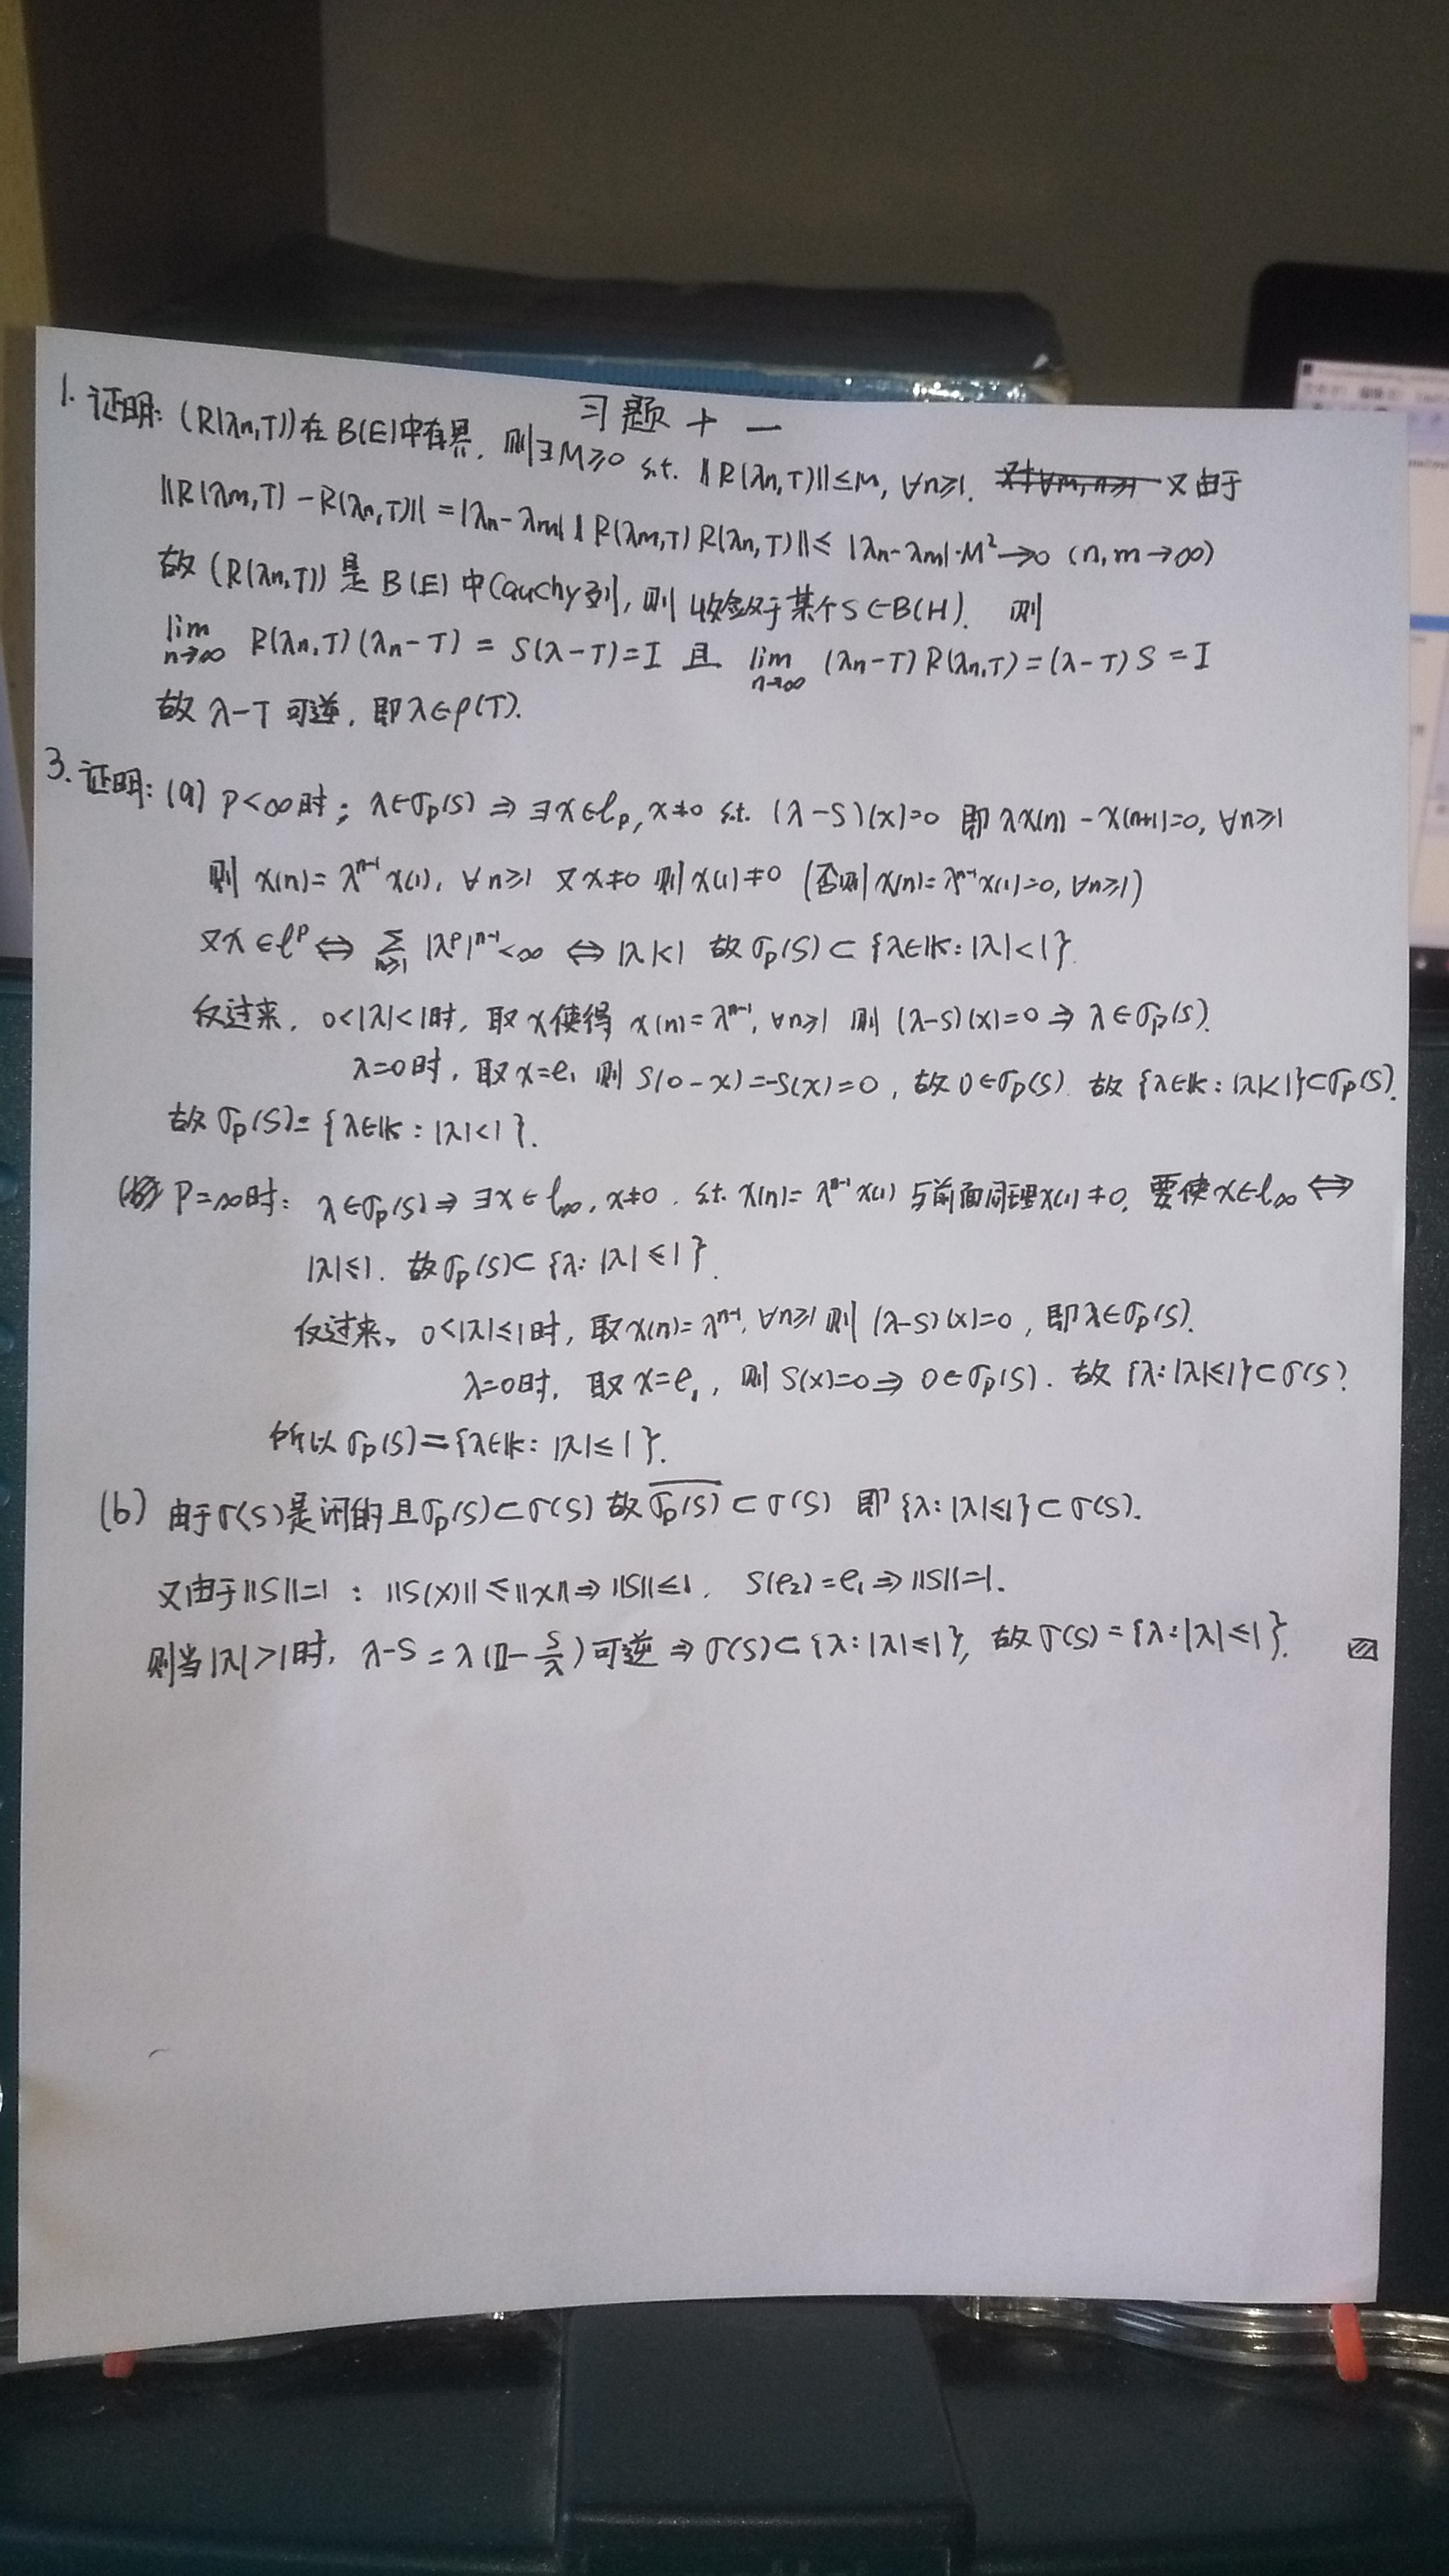
\includegraphics[scale=0.18]{11_1_3.jpg}
\clearpage
4. 设$E$是Banach空间,$T$是$E$上的线性等距映射. 并记
\[D=\{\lambda\in\mathbb{K}:|\lambda<1|\},\ C=\{\lambda\in\mathbb{K}:|\lambda|=1\},\ \overline{D}=D\cup C.\]
\begin{itemize}
	\item[(a)] 证明:$\sigma_p(T)\subset C$, $\sigma(T)\subset \overline{D}$; 并且当$\lambda\in D$时,有
	\[\lambda\in\rho(T)\Leftrightarrow(\lambda-T)(E)=E.\]
	\item[(b)] 假设$(\lambda_n)\subset D\cap \rho(T)$收敛到$D$中的元素$\lambda$. 证明:$\lambda\in\rho(T)$.
	\item[(c)] 证明:$D\cap \rho(T)$在$D$中既是开集又是闭集。由此导出$D\cap\rho(T)$是空集或者$D\cap\rho(T)=D$.
	\item[(d)] 证明:$\sigma(T)$或者包含于$C$中或者等于$\overline{D}$, 并且前者成立的充分必要条件是$T$为满射。
	\item[(e)] 假设$E=\ell_p$, $1\leq p\leq\infty$, 且$T$为$E$上的后移算子:
	\[T(x)(1)=0\text{ 且 }T(x)(n)=x(n-1),n>1.\]
	证明:$\sigma(T)=\overline{D}$并且$\sigma_p(T)=\varnothing$.
\end{itemize}
\begin{proof}
	(a) 设$T$是线性等距映射,即$\|Tx\|=\|x\|$, $\forall x\in E$.
	\begin{itemize}
		\item[(1)] $\lambda\in\sigma_p(T)\RA\exists x\ne 0, (\lambda-T)x=0\RA\lambda x=Tx, |\lambda|\|x\|=\|Tx\|$, 则$\|\lambda\|=1$. 故$\sigma_p(T)\subset C$.
		\item[(2)] 易看出$\|T\|=1$, 则当$\lambda>1$时,$\lambda-T=\lambda(\mathbb{I}-\frac{T}{\lambda})$可逆,故$\sigma\subset\overline{D}$.
		\item[(3)] 设$\lambda<1$. "$\RA$": $\lambda\in\rho(T)\RA\lambda-T\text{ 可逆 }$, 则满射,即$(\lambda-T)E=E$;
		
		"$\LA$": 设$\lambda-T$为满射,若$\lambda-T$不为单射则$\lambda\in\sigma_p(T)$, 那么$|\lambda|=1$这与$|\lambda|<1$矛盾,故$\lambda-T$为单射,所以$\lambda-T$为连续双射,$E$为Banach空间,则由开映射定理知$\lambda-T$可逆,即$\lambda\in\rho(T)$.
	\end{itemize}
	
	(b) ??
	
	(c) $\rho(T)$是$\mathbb{K}$中开集则$D\cap\rho(T)$是$D$中开集;又由(b)知$D\cap\rho(T)$是$D$中闭集,故$D\cap\rho(T)$是$D$中既开又闭。注意到$D$是连通的,故$D\cap\rho(T)$为空集或者$D$.
	
	(d) 当$D\cap \rho(T)=\varnothing$时,$D\subset\sigma(T)$, 则$\overline{D}\subset \sigma(T)$, 又由(a)知$\sigma(T)\subset \overline{D}$, 所以$\sigma(T)=\overline{D}$; 当$D\cap \rho(T)=D$时$D\subset \rho(T)$, 则$\rho(T)\subset \overline{D}\backslash D=C$.
	
	$\sigma(T)\subset C\Leftrightarrow T$为满射:"$\RA$": 设$\sigma(T)\subset C$, 则$0\notin \sigma(T)$, 故$T$可逆,则$T$满射;"$\LA$": 设$T$满射, 若$\sigma\subset T$不成立,则$\sigma(T)=\overline{D}$, 那么$0\in\rho(T)=\overline{D}^c$, 矛盾。 
	
	(e) 没有元素$x$使得$T(x)=e_1$, 所以$T$不是满射,由(d)知这意味着$\sigma(T)=\overline{D}$.
	
	显然$Tx=0\RA x=0$, 故$T$为单射,则$\sigma_p(T)=\varnothing$. 
\end{proof}

8. 设$E$和$F$是赋范空间。证明下面的命题成立:
\begin{itemize}
	\item[(a)] 若$(x_n)$是$E$中的弱收敛序列,则$(x_n)$有界。
	\item[(b)] 若$T\in B(E,F)$且$x_n$弱收敛到$x$, 则$T(x_n)$弱收敛到$T(x)$.
	\item[(c)] 若$T\in B(E,F)$是紧算子且$x_n$弱收敛到$x$, 则$T(x_n)$依范数收敛到$T(x)$.
	\item[(d)] 若$E$自反,$T\in B(E,F)$且当$x_n$弱收敛到$x$时,有$T(x_n)$依范数收敛到$T(x)$, 则$T$是紧算子。
	\item[(e)] 若$E$自反,且$T\in B(E,\ell_1)$或$T\in B(c_0,E)$, 则$T$是紧算子。
\end{itemize}
\begin{proof}
	(a) 一致有界原理。
	
	(b) 设$x_n$弱收敛到$x$, 注意到对任意$f\in F^*$, $f\circ T\in E^*$, 则
	\[f(T(x_n))\to f(T(x)), n\to\infty.\]
	
	(c) 先证明任意赋范空间$F$中任意范数紧的子集$A$上范数拓扑等于弱拓扑:恒等映射$\mathrm{id}: (A,\|\cdot\|)\to (A,\sigma(F,F^*))$为连续双射,又$(A,\|\cdot\|)$紧故$\mathrm{id}$为同胚映射。
	
	由$(x_n)$弱收敛知$(x_n)$有界则存在$M>0$, s.t. $(x_n)\cup \{x\}\subset M B_E$. $T$为紧算子,则$T(MB_E)=MT(B_E)$是范数相对紧的,因此$\overline{T(MB_E)}$上范数拓扑等于弱拓扑,又$T(x_n)$弱收敛到$T(x)$, 则$T(x_n)$依范数收敛到$T(x)$.
	
	(d) 只需证明$T(B_E)$相对紧,则只需证明$T(B_E)$中任意无穷序列都有收敛于$F$中元素的子序列:设$(y_n)$是$T(B_E)$中一个无穷序列,则存在$(x_n)\subset B_E$使得$y_n=T(x_n), \forall n\geq 1$. 由第九章第4题知$(x_n)$有弱收敛于某个$x\in  E$的子列$(x_{n_k})$, 由题设知$T(x_{n_k})$依范数收敛于$T(x)$, 即$(y_{n_k})$依范数收敛于$T(x)\in F$, 故$T(B_E)$相对紧。
	
	(e)先证明$\forall T\in B(E,\ell_1)$是紧算子。由(d)知只需证明当$x_n$弱收敛到$x$时有$T(x_n)$依范数收敛到$T(x)$. 当$x_n$弱收敛到$x$时,$T(x_n)$弱收敛到$T(x)$, 由下面的小结论知$T(x_n)$依范数到$T(x)$.
	
	小结论:$\ell_1$中弱收敛的序列一定依范数收敛:设$(x_n)$弱收敛到$0$, 反证法,假设$(x_n)$不依范数收敛到$0$, 则存在$\e_0>0$, 子列$(x_{n_k})$使得$\|x_{n_k}\|\geq \e_0$, 把$(x_{n_k})$记为$(y_n)$. 由$(y_1^k)\in \ell_1$, 存在$k_1$使得
	\[\sum_{k\geq k_1+1}|y_1^k|<1,\sum_{k\leq k_1}|y_1^k|\geq \|y_1\|-1,\]
	由$(y_n)$弱收敛(则逐点收敛),对于取定的$k_1$, 存在$n_2> 1$使得$\sum_{k\leq k_1}|y_{n_2}^k|<2^{-1}$. 由$y_{n_2}\in\ell_1$知存在$k_2>k_1$使得
	\[\sum_{k\geq k_2+1}|y_{n_2}^k|<2^{-1},\sum_{k_1+1}^{k_2}|y_{n_2}^k|\geq \|y_{n_2}\|-2\cdot 2^{-1},\]
	对于取定的$k_2$, 存在在$n_3>n_2$使得$\sum_{k\leq k_2}|y_{n_3}^k|<\frac{1}{3}$. 
	以此类推,对任意$s\geq 2$, 存在严格增加的$k_s$使得
	\[\sum_{k\leq k_{s-1}}|y_{n_s}^k|<s^{-1}, \sum_{k\geq k_s+1}|y_{n_s}^k|<s^{-1}, \sum_{k_{s-1}+1}^{k_s}|y_{n_s}^k|\geq \|y_{n_s}\|-2\cdot s^{-1}\]
	令$z=(z^k)$满足
	\[
	z^k=\begin{cases}
	\overline{\mathrm{sgn}(y_1^k)}, &k\leq k_1\\
	\overline{\mathrm{sgn}(y_s^k)}, &k_{s-1}+1\leq k\leq k_s, s\geq 2
	\end{cases}
	\]
	则对任意$s\geq 1$有:
	\[|\la z,x_{n_s}\ra|\geq \sum_{k_{s-1}+1}^{k_s}z^ky_{n_s}^k-|\sum_{k\leq k_{s-1}}z^ky_{n_s}^k|-|\sum_{k\geq k_{s}+1}z^ky_{n_s}^k|\geq \|y_{n_s}\|-4\cdot s^{-1}\geq \e_0-4\cdot s^{-1}\]
	当$s$充分大时$\e_0-4\cdot s^{-1}>\e_0\backslash 2$, 故$(y_{n_s})$不是弱收敛的,矛盾。
	
	至此我们说明了任意自反空间到$\ell_1$的任意有界算子是紧算子. 另一方面,对任意$T\in B(c_0,E)$, 则$T^*\in B(E^*,(c_0)^*)=B(E^*,\ell_1)$, 由$E^*$仍然是自反的,则$T^*$是紧算子,所以$T$是紧算子. 证毕.
\end{proof}

\begin{Prop}
	Let $X,Y$ be two normed spaces, $L:X\to Y$ linear operator. If for any functional $\varphi\in X^*$, $\varphi\cdot L$ is bounded, than $L$ is bounded.
\end{Prop}



存在特征为素数的无限域, 如$\mathbb{Z}_p(x)$.

《高等代数学习指导下册》 p168-169. 关于域的特征。


Polar Decomposition:

$|X|(|X|+\epsilon I)^{-1}$ is uniformly bounded in norm by $1$ for $\e>0$. I'll show you that
\[s-\lim_{\epsilon\downarrow 0}|X|(|X|+\epsilon I)^{-1} = P,\]
where $P$ is the orthogonal projection onto the closure of the range of $|X|$. That's enough to give you what you want because $VP=V$(because $V=V(P+P_{\ker X})=VP$) and
\[X(|X|+\epsilon I)^{-1}=V|X|(|X|+\epsilon I)^{-1}\]
So that's the plan.

Because of the uniform bound on the operator norm of $|X|_{\epsilon}=|X|(|X|+\epsilon I)^{-1}$, it is enough to show that $|X|_{\e}$ converges strongly as $\e\to 0^+$ on a dense set subspace of $H$ to $P$. The dense subspace of interest here is
\[\mathcal{M}=\mathcal{R}(|X|)\oplus\mathcal{N}(|X|).\]
This is dense because $\mathcal{R}(|X|)^{\perp}=\mathcal{N}(|X|)$. Notice that $|X|_{\e}$ is $0$ on $\ker(|X|)$; so the only challenge is the strong limit on $R(|X|)$. However, if $x=|X|z$ for some $z$,
\[\begin{aligned}
	|X|(|X|+\epsilon I)^{-1}x & =x-\epsilon(|X|+\epsilon I)^{-1}x \\
	& = x -\epsilon|X|(|X|+\epsilon I)^{-1}z.
\end{aligned}\]
The right side converges to $x$ as $\e\to 0^+$ because of the uniform operator norm bound on $|X|(|X|+\epsilon I)^{-1}$. So that's enough to show that
\[s-\lim_{\epsilon\downarrow 0}|X|(|X|+\epsilon I)^{-1} = P \\
\implies s-\lim_{\epsilon\downarrow 0}X(|X|+\epsilon I)^{-1} = VP=V.\]

\end{document}
